% main.tex -- main text of the article.  The Supplementary Material is supplement.tex.
% Compile (one latexmk at a time):  latexmk -pdf main.tex; latexmk -pdf supplement.tex; latexmk -pdf main.tex
% (pdflatex + bibtex; TeX Live 2025).  Cross-references between the two documents use xr-hyper: in this file the
% prefix S- refers to supplement.aux, in supplement.tex the prefix M- refers to main.aux.
% Every quantitative statement in main.tex and sections/*.tex carries a comment  % src: <path> (<key>)
% pointing at the results file or script it comes from; paths are relative to the repository root.
\documentclass[11pt,a4paper]{article}

\usepackage[T1]{fontenc}
\usepackage[utf8]{inputenc}
\usepackage{lmodern}
\usepackage[a4paper,margin=2.5cm]{geometry}
\usepackage{amsmath,amssymb,amsthm}
\usepackage{graphicx}
\usepackage{booktabs}
\usepackage{array,longtable,multirow}
\usepackage{enumitem}
\usepackage[font=small,labelfont=bf]{caption}
\usepackage{microtype}
\usepackage[numbers,sort&compress]{natbib}
\usepackage{xcolor}
\usepackage{xr-hyper}
\usepackage[colorlinks=true,linkcolor=blue!50!black,citecolor=blue!50!black,urlcolor=blue!50!black]{hyperref}
\externaldocument[S-]{supplement}

\usepackage[section]{placeins}   % floats stay inside the section that defines them

\renewcommand{\topfraction}{0.92}
\renewcommand{\bottomfraction}{0.80}
\renewcommand{\textfraction}{0.06}
\renewcommand{\floatpagefraction}{0.75}
\setcounter{topnumber}{3}
\setcounter{bottomnumber}{2}
\setcounter{totalnumber}{4}

\hypersetup{pdftitle={Random-walk SIR models of indoor epidemics: reproduction numbers, discrete individuals
  and pre-specified tests against outbreaks, contact records and tracer measurements},
  pdfauthor={Xiaoxiao Zhouyi},
  pdfkeywords={indoor transmission; lattice random walk; basic reproduction number; next-generation matrix;
  pair-level theory; stochastic simulation; outbreak data; contact networks; tracer measurements;
  pre-specified test}}

\graphicspath{{figures/}}
% macros.tex -- notation and theorem environments of the article and its Supplementary Material.
% Loaded by main.tex and supplement.tex after amsmath, amssymb, amsthm.  The notation is typeset as Table "appD_tables:tab:notation"
% (Supplementary Section S1); the comment table below adds, in its last column, the names used in the code.
%
% =====================================================================================================
% NOTATION TABLE (mapping to the code in the last column)
% -----------------------------------------------------------------------------------------------------
%  symbol            macro            meaning                                             code
% -----------------------------------------------------------------------------------------------------
%  \Omega            \cells           set of walkable lattice cells (barriers removed)    Omega
%  n                 \ncell           number of walkable cells, n = |\Omega|              n (theory), M or |Omega| (sim)
%  x, y, z           --               cells (elements of \Omega)                          r, s (theory); x, y (sim)
%  a                 --               lattice spacing (m); lengths in cells unless stated a
%  D_x               --               mobility (diffusion coefficient) of cell x, cell^2/day   D(r)
%  D_0               \Dz              mobility scale: D_x = D_0 d_x, d_x the zone multiplier    D0
%  \omega_{x\to y}   \hop{x}{y}       hop rate from x to a neighbouring cell y (1/day)    w_{s->r}, W(x->y)
%  \mathbf M         \gen             movement generator, M_{yx} = \omega_{x\to y}, 1^T M = 0   M (theory), L (sim)
%  \mathbf M_0       \genz            generator at D_0 = 1, so M = D_0 M_0
%  \boldsymbol\pi    \stat            stationary distribution of M (uniform for the symmetric rule)  pi
%  P_t(y|x)          --               propagator, (e^{Mt})_{yx}                           P_t(r|s), G
%  q_x, \mathbf Q    \Qm              infection efficiency of cell x; Q = diag(q)         q, Q
%  \beta, \gamma     --               transmission rate, recovery rate (1/day)
%  \mathbf P         \ker             contact kernel, row-stochastic, P_{xy} = P(y|x)     P (sim)
%  N                 \Npop            number of people in the room                        N, N_tot
%  S_x, I_x, R_x     --               expected numbers of susceptible/infective/recovered in cell x
%  \mathbf J         \Jm              growth operator J = M + F - \gamma 1                J
%  \mathbf F, \mathbf V  \Fm, \Vm     transmission and transition parts; F = \beta P^T Q (= \beta Q for the same-cell kernel), V = \gamma 1 - M
%  \mathbf K         \ngm             next-generation matrix K = F V^{-1}                 K
%  n_off(x)          \noff            offspring number: column sum of K (mean-field secondary cases of a case born at x)
%  R_0               \Rz              basic reproduction number of the mean-field model, \rho(K)
%  \lambda_1         \lamone          growth rate s(J)                                    lambda_1
%  s(A), \rho(A)     \sabs, \srad     spectral abscissa, spectral radius
%  <q>_\pi           \qmean           \sum_x \pi_x q_x  (plain <q> when \pi is uniform)   <q>_pi
%  q_max, q_min      \qmax, \qmin
%  u, \ell           \uvec, \lvec     right/left Perron vectors of J (prevalence map; u sums to 1)   u, l
%  w, z              \wvec, \zvec     right/left Perron vectors of K (incidence map; reproductive value)   w, z  (sim: v, u)
%  e_x               \evec            elasticity map, e_x = d ln R0 / d ln q_x            e
%  \mathcal E(v)     \dirich          Dirichlet form of the reversible generator          E(x)
%  \mu_k, \phi_k     --               eigenvalues/eigenvectors of -M (reversible case), \mu_0 = 0
%  Z, \mu_Z          \muZ             a set of cells (zone); exit rate \mu_Z = -s(M[Z,Z])
%  \kappa_x          --               exit (door) rate from cell x; M_\kappa = M - diag(\kappa)
%  \mu_leak          \muk             leak rate, -s(M_\kappa)
%  R_0^{room}        \Rroom           reproduction number of a leaky room
%  \bar\rho          \rhobar          mean number of OTHER people per cell, (N-1)/n       rho_bar
%  h(x,y)            --               pair hazard \beta q_x P(y|x)/\bar\rho               h
%  p(x,y)            --               probability that a case born at x infects a given person then at y
%  R_1(x)            \Rone            expected secondary cases of a lone index case born at x (pair level)
%  \bar R_1          \Ronebar         R_1 averaged over a uniformly placed index case      "pair R1", "R1 uniform index"
%  \mathbf K_1       \ngmone          pair-level next-generation matrix                   K1
%  g_0               \gz              Laplace-transformed return probability of the relative walk at \gamma
%  c_x               --               encounter factor of the per-cell rule
%  \hat R            \Rhat            counted mean number of secondary cases in simulation
%  f                 --               fraction of the day a room is occupied (duty cycle)
%  M0, M1, M2        \Mzero,\Mone,\Mtwo  validation models: well mixed; same-site; with non-local airborne term
%  \varepsilon_k     --               infectiousness parameter of outbreak event k
%  X_j               --               model exposure of susceptible j
%  D_p, D_{air}      \Dp, \Dair       calibrated mobility of people (M1) and mixing coefficient of quanta (M2), m^2/h
%  \Lambda           \remrate         removal rate of airborne quanta (ventilation + deposition + inactivation), 1/h
% -----------------------------------------------------------------------------------------------------
%  Units: time in days and lengths in lattice cells in Sections 2-6 (D in cell^2/day, a = 1);
%         hours and metres in Section 7 (D_p, D_air in m^2/h).
%  Default epidemiological parameters: \beta = 0.5/day, \gamma = 0.14/day.
% =====================================================================================================

% --- sets, vectors, matrices
\newcommand{\cells}{\Omega}
\newcommand{\ncell}{n}
\newcommand{\Npop}{N}
\newcommand{\Dz}{D_0}
\newcommand{\hop}[2]{\omega_{#1\to #2}}
\newcommand{\gen}{\mathbf{M}}
\newcommand{\genz}{\mathbf{M}_0}
\newcommand{\genk}{\mathbf{M}_{\kappa}}
\newcommand{\stat}{\boldsymbol{\pi}}
\newcommand{\Qm}{\mathbf{Q}}
\renewcommand{\ker}{\mathbf{P}}          % contact kernel (the operator \ker is not used in this article)
\newcommand{\Jm}{\mathbf{J}}
\newcommand{\Fm}{\mathbf{F}}
\newcommand{\Vm}{\mathbf{V}}
\newcommand{\ngm}{\mathbf{K}}
\newcommand{\ngmone}{\mathbf{K}_1}
\newcommand{\Id}{\mathbf{1}}             % identity matrix
\newcommand{\one}{\boldsymbol{1}}        % vector of ones
\newcommand{\uvec}{\mathbf{u}}
\newcommand{\lvec}{\boldsymbol{\ell}}
\newcommand{\wvec}{\mathbf{w}}
\newcommand{\zvec}{\mathbf{z}}
\newcommand{\evec}{\mathbf{e}}
\newcommand{\qvec}{\mathbf{q}}
\newcommand{\T}{\mathsf{T}}              % transpose
\newcommand{\diag}{\operatorname{diag}}

% --- spectral quantities and reproduction numbers
\newcommand{\sabs}{s}                    % spectral abscissa s(A)
\newcommand{\srad}{\rho}                 % spectral radius \rho(A)
\newcommand{\Rz}{R_0}
\newcommand{\Rroom}{R_0^{\mathrm{room}}}
\newcommand{\Rone}{R_1}
\newcommand{\Ronebar}{\bar{R}_1}
\newcommand{\Rhat}{\widehat{R}}
\newcommand{\lamone}{\lambda_1}
\newcommand{\qmean}{\langle q\rangle_{\pi}}
\newcommand{\qmax}{q_{\max}}
\newcommand{\qmin}{q_{\min}}
\newcommand{\muZ}{\mu_Z}
\newcommand{\muk}{\mu_{\mathrm{leak}}}   % leak rate (not \mu_\kappa: too close to \mu_k in print)
\newcommand{\noff}{n_{\mathrm{off}}}      % offspring number (column sum of K)
\newcommand{\dirich}{\mathcal{E}}
\newcommand{\rhobar}{\bar{\rho}}
\newcommand{\gz}{g_0}

% --- validation models and parameters
\newcommand{\Mzero}{\mathrm{M0}}
\newcommand{\Mone}{\mathrm{M1}}
\newcommand{\Mtwo}{\mathrm{M2}}
\newcommand{\Dp}{D_{\mathrm{p}}}
\newcommand{\Dair}{D_{\mathrm{air}}}
\newcommand{\remrate}{\Lambda}

% --- probability
\newcommand{\Prob}{\mathbb{P}}
\newcommand{\Exp}{\mathbb{E}}
\newcommand{\dd}{\mathrm{d}}
\newcommand{\e}{\mathrm{e}}

% --- units and small helpers
\newcommand{\perday}{\,\mathrm{day}^{-1}}
\newcommand{\cdunit}{\ensuremath{\mathrm{cell}^2\,\mathrm{day}^{-1}}}   % the unit of mobility, in text or math
\newcommand{\cellday}{\ensuremath{\,\mathrm{cell}^2\,\mathrm{day}^{-1}}} % the same after a number
\newcommand{\pct}{\,\%}                                                  % per cent after a number
\newcommand{\sqmh}{\,\mathrm{m}^2\,\mathrm{h}^{-1}}
\newcommand{\qph}{\,\mathrm{quanta}\,\mathrm{h}^{-1}}

% --- theorem environments (one counter per section; numbering Theorem 3.1, Proposition 3.2, ...)
\theoremstyle{plain}
\newtheorem{theorem}{Theorem}[section]
\newtheorem{proposition}[theorem]{Proposition}
\newtheorem{lemma}[theorem]{Lemma}
\newtheorem{corollary}[theorem]{Corollary}
\newtheorem{conjecture}[theorem]{Conjecture}
\theoremstyle{definition}
\newtheorem{definition}[theorem]{Definition}
\newtheorem{assumption}{Assumption}
\renewcommand{\theassumption}{\Alph{assumption}}
\newtheorem{observation}[theorem]{Numerical observation}
\newtheorem{example}[theorem]{Example}
\theoremstyle{remark}
\newtheorem{remark}[theorem]{Remark}

% Generated table bodies (data/v2_tab_*.tex, written by code/v2_numbers.py) are read with the primitive \input,
% which is expandable, so that a rule may follow the last row.
\makeatletter
\newcommand{\tabinput}[1]{\@@input #1.tex }
\makeatother


% State of the repository named in the availability statement.  make_release.py tests the URL and the
% version tag when the release is built and writes repo_status.tex (\repopublictrue, \repotaggedtrue as
% found); without that file the cautious wording is used.
\newcommand{\repoversion}{1.2.0}
\newif\ifrepopublic
\repopublicfalse
\newif\ifrepotagged
\repotaggedfalse
\InputIfFileExists{repo_status.tex}{}{}

\title{Random-walk SIR models of indoor epidemics:\\ reproduction numbers, discrete individuals and\\
pre-specified tests against outbreaks, contact records\\ and tracer measurements}

\author{Xiaoxiao Zhouyi\\[4pt]
\normalsize School of Engineering Mathematics and Technology, University of Bristol, UK\\
\normalsize \href{mailto:zhouyixiaoxiao@gmail.com}{zhouyixiaoxiao@gmail.com}}

\date{\vspace{-1.5ex}2026\vspace{-2ex}}

\begin{document}
\maketitle

\begin{abstract}
We study SIR epidemics of independent random walkers on a lattice with cell-dependent mobility and
infection efficiency. (i)~The mean-field $\Rz$ is the spectral radius of a next-generation matrix of
the lattice propagator. For same-cell transmission its bounds, limits and monotone decrease in mobility hold, as
known for patch models; for other kernels the lower bound and monotonicity can fail. With uniform efficiency,
$\Rz$ of a closed room is independent of size, shape and mobility; a leak replaces $\gamma$ by $\gamma+\muk$
under stated conditions.
(ii)~Two-walker theory gives the exact mean number of first-generation secondary cases of a lone index case;
it lies below $\Rz$ at low occupancy and mobility (office scene: 2.27 against 5.11) and is not a threshold.
% src: data/s5_pair_large_sample.json (office|D0=1: R1bar_exact 2.2661, counted 2.265 +- 0.004 in 400,000 runs, R0_ngm 5.1073; office|D0=100: R1bar_exact 4.3411, R0_ngm 4.646)
(iii)~In exact simulations of four closed-room scenes, spatial effects are large only at very low mobility.
(iv)~Five tests, with protocols fixed before the tested model was run (data-aware,
self-attested, not registered), confront the model with 22 of 38 outbreak records, contact records, tracer
measurements and a school epidemic. There is no general agreement. Same-site transmission is not supported;
walk-generated contacts fail in all six contact datasets. An airborne extension predicts held-out distance
gradients better than a well-mixed model (log-score gain $+14.35$; a constant near/far ratio would also do so with
probability 0.65--0.73), but the pre-specified pooled
comparison favours the constant ratio ($-9.15$, nine-tenths from one event whose near zone was chosen on its data); on four held-out flights they tie. Attack rates are fitted; cell-dependent mobility
remains untested.
% src: data/bsc_outbreaks/outbreaks.csv (27 rows); code/bsc_validation2/a1_more_outbreaks/PREREGISTRATION.md section 2.1 (11 records); 22 records in a test: 2 + 5 (first), 6 + 5 (second), and T3, C3, S1, T7 in the level checks and negative controls of the first test (outbreaks.csv protocol_role); data/v2_numbers.json (con.ladder: A0 on all six datasets); data/v2_numbers.json (out2.pooled.M2.all: delta0 14.351, deltaC -9.150; out2.pooled.plant_share_of_deltaC 0.916; out2.pooled.M2.air: deltaC -0.77; out2.power.registered: CRR P_B1 0.652; out2.power.corrected: CRR B1 0.732); notes/VERIFICATION.md section 4.10 (statement and reservations)
% src: data/s2_model_scenes.json (scenes.<name>.R0_1m: excess over the well-mixed value below 0.03 % at walking mobility)
\end{abstract}

\noindent\textbf{Keywords:} indoor transmission; lattice random walk; basic reproduction number;
next-generation matrix; pair-level theory; stochastic simulation; outbreak data; contact networks; tracer
measurements; pre-specified test.

\section{Introduction}\label{s1_intro:sec}
% Main text, Section 1 (Introduction).
% Paths in "% src:" comments are relative to the repository root.

Recorded clusters of SARS-CoV-2 infection arose overwhelmingly indoors
\citep{qian2021indoor,leclerc2020settings}, and in several well-documented events the cases were not spread
evenly over the room. They sat on one side of a call-centre floor \citep{park2020}, close to the index case in
an aircraft cabin \citep{khanh2020} or on high-speed trains \citep{hu2021}, or at neighbouring restaurant
tables in the air stream of one air conditioner \citep{lu2020,li2021}.
The standard quantitative tool for indoor risk is the Wells--Riley equation
\citep{wells1955airborne,riley1978,szeto2010review}. It and the models built on it
\citep{noakes2006modelling,bazant2021guideline} treat the room air as well mixed, so that every susceptible
occupant carries the same risk.
This article examines what a minimal spatial model adds to that picture: a
susceptible--infective--recovered (SIR) epidemic among people who perform independent random walks on a
lattice of floor cells, with a mobility $D_x$ and an infection efficiency $q_x$ that depend on the cell
(workstations, corridors, meeting rooms, barriers).

\paragraph{Prior work.}
Epidemics among moving individuals have been modelled for more than three decades: lattice automata whose
individuals move between sites \citep{boccara1992automata,rhodes1996persistence}, agents moving in continuous
space \citep{gonzalez2004scaling,frasca2006dynamical,buscarino2008disease}, and reaction--diffusion processes
on metapopulation networks \citep{colizza2007reaction,belik2011natural,wang2014spatial}.
Closest to the present model is the random-walk theory of transmission between two walkers, in which infection
is a reaction that takes place at a finite rate when an infected and a susceptible walker meet
\citep{kenkre2014theory,sugaya2018analysis,kenkre2021theory}. \citet{giuggioli2022spatio} formulate it on a
lattice with exact propagators \citep{giuggioli2020exact,sarvaharman2023particle} and predict a basic
reproduction number analytically for moving susceptible, infected and recovered individuals.
The many-walker system itself is a classical object of probability and of statistical physics. For
independent continuous-time random walkers on $\mathbb{Z}^d$, with infection when an infected and a healthy
walker meet, \citet{kesten2005spread,kesten2008shape} proved that the infected set grows linearly in time with
an asymptotic shape, and, when infected walkers recover and can be infected again, that there is a critical
recovery rate below which the infection survives with positive probability and above which it dies out
\citep{kesten2006phase}. The same process is studied in physics as the diffusive epidemic process, whose
absorbing-state transition has been analysed by mean-field theory and simulation \citep{maia2007diffusive};
with permanent immunity, as here, simulations on the square lattice show a transition of dynamic-percolation
type controlled by the density of walkers \citep{carvalho2025generalized}. These results concern infinite or
large homogeneous lattices. They establish that a threshold exists for walkers; they do not give its value
for the small heterogeneous rooms considered here.
% src: data/refs_search.json (kesten2005spread, kesten2006phase, kesten2008shape, maia2007diffusive, carvalho2025generalized: Crossref records, abstracts in manual_checks; search queries of 1 October 2026)

For compartmental models the basic reproduction number $\Rz$ is the spectral radius of the next-generation
operator \citep{diekmann1990definition}, $\Rz=\srad(\Fm\Vm^{-1})$, and it is a threshold
\citep{vandendriessche2002reproduction}. Linearised at the disease-free state, the mean-field version of the
lattice model is an epidemic patch model with standard incidence, and the relevant theorems are published.
For the patch model with symmetric movement, \citet{allen2007asymptotic} defined $\Rz=\srad(\Fm\Vm^{-1})$,
proved the threshold property, showed that the growth bound $\sabs(\Fm-\Vm)$ decreases with the dispersal rate
between its two limits, and conjectured the same monotonicity for $\Rz$; the conjecture was proved by
\citet{gao2019travel} for symmetric movement and by \citet{gao2020fast} in general (see also
\citet{chen2020asymptotic}), and it is an instance of the reduction principle of
\citet{altenberg2012resolvent}. That $\Rz$ lies between the smallest and the largest patch reproduction
number, and does not depend on movement when they coincide, is due to \citet{gao2011sis}; the sharper lower
bound, which is the fast-dispersal limit, is due to \citet{gao2020fast}, and the approach to that limit at
order one over the dispersal rate was obtained by \citet{tien2015disease}, for a network on which the pathogen
rather than the hosts moves, with a next-generation matrix of the same form. Continuum counterparts are given
by \citet{allen2008asymptotic} and \citet{wang2012basic}. (We read the published versions of
\citet{gao2011sis} and \citet{tien2015disease}, whose Proposition~2.2 and Section~4.2 contain the results
attributed to them, and of \citet{gao2020fast}. For \citet{allen2007asymptotic} and \citet{gao2019travel} we
read only the abstracts; what we attribute to them follows the account of \citet{gao2020fast} and agrees with
the abstracts as far as they go: the threshold property in the first, the monotone decrease in the dispersal
rate for symmetric movement in the second.)
% src: data/refs_search.json (gao2020fast_published: Theorems 2.1, 2.3, 3.3, Corollary 3.5 "generalization of Lemma 3.4 in Allen et al.", Discussion on Tien et al.; checked 1 October 2026)
% src: published versions of doi:10.1016/j.mbs.2011.05.001 (Proposition 2.2: max{max_i tilde R0^(i), min_i R0^(i)} <= R0 <= max_i R0^(i)) and doi:10.1007/s00285-014-0791-x (Section 4.2, eqs. (29)-(35): first-order Laurent correction of R0 in 1/d_W with the generalised group inverse X_0), author copies read 2 October 2026
% src: abstracts of doi:10.1137/060672522 and doi:10.1137/18M1211957 in their Crossref records (read 2 October 2026)

Spatially resolved indoor models also exist: zonal ventilation models \citep{noakes2009mathematical},
transport models for the airborne concentration \citep{lau2022predicting,vuorinen2020modelling}, and
pedestrian- or agent-based simulations of supermarkets and of air travel
\citep{ying2021modelling,namilae2017multiscale}. They resolve the air or the trajectories in more detail than a
lattice walk does. What the lattice model offers in return is analytical access to reproduction numbers; what
it lacks, as Section~\ref{s8_outbreaks:sec} shows, is an adequate description of seated people who share air
and of who meets whom.

Three bodies of measurement bear on such a model, and each has its own literature. Close-range contacts
between people indoors have been recorded with wearable sensors in schools, offices, hospitals and
conferences; they are concentrated on few, repeated partners, structured by groups and broadly distributed in
duration \citep{cattuto2010dynamics,stehle2011high,genois2015data,genois2018can}; random walkers in a plane
that slow down near attractive individuals reproduce several of these statistics
\citep{starnini2013modeling}; and epidemics have been simulated on the recorded networks
\citep{stehle2011simulation,gemmetto2014mitigation}. The transport of
aerosol in vehicles has been measured with tracers \citep{kinahan2021aerosol,woodward2022evaluation,ou2022},
and turbulent diffusion coefficients of rooms have been related to their ventilation
\citep{cheng2011modeling}. And outbreak investigations report risk by distance: contact tracing on aircraft
uses a zone of two rows around a case, a rule whose limits are known \citep{hertzberg2016risk}, and
transmission of influenza in schools has been resolved into classes, grades and schools
\citep{endo2021within}. These are the data against which the model is tested in
Section~\ref{s8_outbreaks:sec}; the rules they suggest, a constant ratio of near to far risk and a fixed share
of contact within the group, are the generic competitors that the model has to beat.

\paragraph{Contributions.}
\begin{enumerate}[label=(\roman*),leftmargin=2.2em,itemsep=1pt,topsep=3pt]
\item \emph{Mean-field reproduction number} (Sections~\ref{s3_r0:sec} and~\ref{s4_geometry:sec}). We state
  and prove that $\Rz=\srad\bigl(\beta\Qm(\gamma\Id-\gen)^{-1}\bigr)$, a next-generation matrix built from the
  Laplace-transformed lattice propagator. For same-cell transmission we prove that
  $\beta\qmean/\gamma\le\Rz\le\beta\qmax/\gamma$, that $\Rz$ decreases monotonically with the mobility scale
  between these limits, and that any high-risk zone contributes a lower bound; the lower bound and the
  monotonicity can fail for other contact kernels. In a closed room with uniform $q$, $\Rz$ does not depend on
  the size or shape of the room. The genuine boundary effect is a leak (doors, finite dwell
  time): for uniform $q$ and the same-cell kernel, or for a dwell time that does not depend on position and
  any kernel, it replaces $\gamma$ by $\gamma+\muk$, and for heterogeneous $q$ and the same-cell kernel it
  gives $\beta\langle q\rangle_\nu/(\gamma+\muk)\le\Rroom\le\beta\qmax/(\gamma+\muk)$
  (Theorem~\ref{s4_geometry:thm:leaky}); for other kernels and a localised door the formula and both bounds
  can fail.
\item \emph{Discrete individuals} (Section~\ref{s5_pair:sec}). Following the two-walker theory of
  transmission \citep{kenkre2014theory,giuggioli2022spatio}, infection is treated as a partially absorbing
  defect of the two-walker process. This gives the expected number of secondary cases $\Rone(x)$ of an index
  case and a closed form for homogeneous periodic rooms and the infinite floor, which approximates rooms with
  reflecting walls to within 1\,\% in the cases tested. It explains why counted secondary cases fall below
  $\Rz$ at low occupancy and what form a finite-size effect takes for discrete people.
  % src: data/s5_pair_checks.json (finite_size: largest deviation of the closed form from the exact pair solve 0.90 %, 21 rooms)
\item \emph{Exact stochastic simulation} (Section~\ref{s6_scenes:sec}) of four scenes (office, supermarket,
  classroom, metro carriage) and of interventions, in which secondary cases are counted from the infection
  tree and not fitted.
\item \emph{Confrontation with data} (Section~\ref{s8_outbreaks:sec}). We assemble 38
  records of documented indoor outbreaks and exposure cohorts: a first dataset of 27 records from 31
  published sources (23 with counts of cases and of exposed people) and a second dataset of eleven records of ten
  outbreaks with seat or position data. Two spatial models ($\Mone$, $\Mtwo$) are tested against a well-mixed
  model ($\Mzero$) on 18 of them in two out-of-sample tests (two records for calibration and five held out;
  then six and five; four further records enter the level checks and negative controls of the first test) and, in the second test by design, against a constant ratio of near to far risk. Three
  further analyses address what outbreak counts cannot: contacts generated by the lattice walk are compared
  with recorded contacts in six indoor settings; the airborne kernel is fixed by published tracer measurements
  and then confronted with the outbreaks; and the model reduced to zones, with mixing measured in one school,
  is used to predict an influenza epidemic in 29 others. Each of the five primary tests follows a protocol
  written before the model under test was run on its data (for the tracer analysis, on outbreaks whose outcome
  under the other models was already known). The protocols are pre-specified, not pre-registered in the usual
  sense: they were written with the data already known, they were not lodged with a registry, and their timing
  is attested by file hashes and file times only. Comparisons added after the results were known are marked
  as post hoc, and a register of all tests says which were specified in advance
  (Supplementary Table~\ref{S-appS_prot2:tab:register}). Everything is reported with its failures.
  % src: data/bsc_outbreaks/outbreaks.csv (27 rows); code/bsc_validation2/a1_more_outbreaks/PREREGISTRATION.md section 2.1; notes/VERIFICATION.md (Section 4.4, outbreak dataset); notes/VERIFICATION.md (Section 4.5, first outbreak test: pre-registration data-aware, model-blind); notes/VERIFICATION.md section 4.10 (reservations)
\end{enumerate}

\paragraph{What is known and what is added.}
Table~\ref{s1_intro:tab:known} separates the two. The theorems on the mean-field $\Rz$ are known for patch
models. We give complete proofs from standard facts on non-negative matrices (Supplementary
Section~\ref{S-appS_r0:sec}) because the conditions matter: the lower bound $\beta\qmean/\gamma\le\Rz$ holds for
the same-cell kernel and fails for general contact kernels, for which we give a three-cell counter-example
(Proposition~\ref{s3_r0:prop:kernel}).
% src: data/plan_theory_checks.json (checks: kernel_counterexample, 0.50 against mean q 0.667)
The two-walker formalism is prior work, and the saturation of contacts between neighbours that it captures
is a classical effect \citep{ball1997epidemics,keeling1999effects,durrett1994importance}. In particular,
\citet{giuggioli2022spatio} already derive the mean number of secondary infections of one infected walker
among uniformly placed susceptible walkers in a closed domain from the two-walker formalism and check it
against simulation; the one-defect solution is that of \citet{szabo1984localized}. What is added here is
narrower (Section~\ref{s5_pair:sec}): the normalisation of the pair hazard by the occupancy, which makes the
pair-level and the mean-field numbers refer to the same model and gives the entrywise comparison
$\ngmone\le\ngm$; the numbers $\Rone(x)$ and the matrix $\ngmone$ for heterogeneous rooms with contact
kernels; the closed form for periodic rooms and the infinite floor with its limits; the comparison with the
second generation; and the observation that neither $\Ronebar$ nor the spectral radius of $\ngmone$ is a
threshold quantity (Remark~\ref{s5_pair:rem:threshold}). These statements of what is added rest on a targeted
search (Crossref and arXiv queries on infection among random walkers, the diffusive epidemic process and
patch-model reproduction numbers, 1~October 2026), not on a systematic review.
% src: data/refs_search.json (searches: queries and numbers of records screened)

\begin{table}[tbp]
\centering\small
\caption{Results of this article, where they are known from, and what is added here. `Thm' numbers refer
to the published version of \citet{gao2020fast}. No novelty is claimed for rows 1--6 and~8; in rows 9
and~10 the data are those of the cited sources; what is added is their compilation and digitisation and the
tests.}
\label{s1_intro:tab:known}
\begin{tabular}{@{}>{\raggedright\arraybackslash}p{0.27\textwidth}>{\raggedright\arraybackslash}p{0.31\textwidth}>{\raggedright\arraybackslash}p{0.35\textwidth}@{}}
\toprule
Result & Known from & Added here \\
\midrule
1.\ $\Rz=\srad(\Fm\Vm^{-1})$ and its threshold property &
  \citep{diekmann1990definition,vandendriessche2002reproduction}; for the patch model
  \citep{allen2007asymptotic} &
  proof in lattice notation; the modal formula, of which the largest diagonal term is a lower bound \\\addlinespace[2pt]
2.\ $\beta\qmean/\gamma\le\Rz\le\beta\qmax/\gamma$ &
  between the smallest and largest patch numbers \citep{gao2011sis}; lower bound \citep{gao2020fast} Thm~3.3;
  continuum case \citep{allen2008asymptotic}; heterogeneity raises $\Rz$ \citep{hasibeder1988population} &
  the condition (same-cell kernel) and a counter-example for other contact kernels \\\addlinespace[2pt]
3.\ $\Rz$ decreases with mobility, between the limits of row~2 &
  conjectured in \citep{allen2007asymptotic}; proved in \citep{gao2019travel} (symmetric movement) and
  \citep{gao2020fast} Thm~2.3 (general); \citep{chen2020asymptotic,altenberg2012resolvent} &
  size of the effect in four indoor scenes, at low and at realistic mobility \\\addlinespace[2pt]
4.\ Uniform $q$: $\Rz=\beta q/\gamma$ whatever the movement &
  \citep{gao2011sis}; loss through absorbing boundaries \citep{skellam1951random,cantrell2003spatial} &
  consequence for rooms (no size effect when closed); leaky-room formula $\Rroom=\beta q/(\gamma+\muk)$
  (same-cell kernel) \\\addlinespace[2pt]
5.\ Zone lower bound; expansions for fast and slow mixing; edge-wise monotonicity &
  fast-dispersal expansion \citep{tien2015disease}; the others are elementary consequences of the same matrix
  theory, for which a targeted search found no source &
  statements and proofs for indoor lattices \\\addlinespace[2pt]
6.\ Hotspot maps (Perron vectors, elasticities) &
  standard eigenvector sensitivity &
  application to the scenes; a caveat on transients \\\addlinespace[2pt]
7.\ Infection as a reaction between two walkers; mean number of secondary infections of one infected
  walker &
  \citep{kenkre2014theory,sugaya2018analysis,giuggioli2022spatio,kenkre2021theory}; one defect
  \citep{szabo1984localized}; local saturation
  \citep{ball1997epidemics,keeling1999effects,durrett1994importance}; thresholds for walkers on
  infinite lattices \citep{kesten2006phase,maia2007diffusive,carvalho2025generalized} &
  occupancy-normalised hazard and $\ngmone\le\ngm$; $\Rone(x)$ and $\ngmone$ for heterogeneous rooms with
  kernels; closed form for periodic rooms and the infinite floor; second generation; not a threshold
  \\\addlinespace[2pt]
8.\ Diffusing-aerosol exposure term; decline of risk with distance &
  \citep{lau2022predicting,venkatram2021modeling,cheng2011modeling}; two-row rule on aircraft
  \citep{hertzberg2016risk} &
  used only as the extension tested in Section~\ref{s8_outbreaks:sec}; no claim that it predicts better than a
  constant ratio \\\addlinespace[2pt]
9.\ Outbreak investigations &
  the published sources of Supplementary Section~\ref{S-appB_dataset:sec}; an earlier compilation of outbreaks
  evaluated with a well-mixed model \citep{peng2022practical} &
  38 records: near/far strata for eight records of the first dataset, the seat map of the call centre, the
  seat-offset matrix of the train cohort, and eleven records of the second dataset with seat or position data;
  two pre-specified out-of-sample tests and their outcome \\\addlinespace[2pt]
10.\ Recorded contacts, tracer measurements, class structure of school epidemics &
  \citep{cattuto2010dynamics,stehle2011high,genois2018can,kinahan2021aerosol,woodward2022evaluation,endo2021within};
  walkers that slow down near others \citep{starnini2013modeling} &
  pre-specified tests of the walk's contacts, of the kernel with a measured coefficient and of the zone-level
  reduction against these data, with negative or weak outcomes \\
\bottomrule
\end{tabular}
\end{table}

\paragraph{Findings.}
In the office scene (234 walkable cells, $\beta=0.5\perday$, $\gamma=0.14\perday$, mobility scale
$\Dz=1\cellday$) the mean-field number is $\Rz=5.11$, inside the bounds 4.64--5.36 that hold for every layout
with the same zone fractions.
% src: data/plan_theory_checks.json (office: D0=1.R0 = 5.107; lower_bound 4.643, upper_bound 5.357)
With 100 discrete people, however, a single index case infects on average $\Ronebar=2.27$ others (the exact
pair-level expectation; counted $\Rhat=2.265\pm0.004$, mean $\pm$ standard error over 400{,}000 runs).
% src: data/s5_pair_large_sample.json (office|D0=1: R1bar_exact 2.2661; mean 2.2648, se 0.0039, n_runs 400000)
Half of the introductions die out: the probability of an outbreak reaching 10\,\% of the room is 0.50,
against 0.78 for the mean-field branching process.
% src: data/bsc_sim/03_scenes.csv (office|D0=1|range1m: p_major 0.496 [0.474, 0.518], p_major_branching 0.781)
The two numbers respond to mobility in opposite ways: at $\Dz=10$ and $100\cellday$, $\Rz$ falls to 4.68 and
4.65 while the pair-level number rises to $\Ronebar=3.79$ and $4.34$.
% src: data/s5_pair_large_sample.json (office|D0=10: R0_ngm 4.676, R1bar_exact 3.7934; office|D0=100: R0_ngm 4.646, R1bar_exact 4.3411)
Barriers, separation of zones and capacity limits reduce simulated outbreaks at low mobility and occupancy.
The cause is the discreteness of individuals (an infective can infect each neighbour only once and keeps
meeting the same ones), not a lower $\Rz$: under frequency-dependent transmission a capacity limit leaves
$\Rz$ unchanged, separation of zones raises it, barrier cells leave it unchanged in a room with uniform $q$
(Theorem~\ref{s4_geometry:thm:closed}), and walls between cells cannot lower it
(Theorem~\ref{s3_r0:thm:edges}).
% src: data/s7_interventions_barriers.json (D=1 paired rhoB=0.10|FD attack -0.040 +- 0.003); data/bsc_sim/05_heterogeneity.json (attack_all 0.347 -> 0.231, R0_ngm 4.286 -> 4.972); data/bsc_sim/07_occupancy.json
These effects belong to a narrow physical regime. With 1.5\,m cells, $\Dz=1\cellday$ is a root-mean-square
displacement of about 3\,m in a day; people who walk 5\,\% of the time or all of the time correspond to
$2.4\times10^{3}$ to $4.9\times10^{4}\cellday$, at which the $\Rz$ of the closed office exceeds its well-mixed
value $\beta\langle q\rangle/\gamma=4.64$ by less than 0.003\,\%.
% src: data/plan_theory_checks.json (office.mobility_table: D0 = 2400: +0.0027 %; D0 = 48700: +0.0001 %); data/bsc_theory/worked_examples.json (E9_physical_D: 2433.6 and 48672 cell^2/day)
Residence time matters as well: if the office is occupied 8 hours a day instead of 24, an index case infects
on average 0.89 to 0.93 people at $\Dz=1$ and 1.34 to 1.40 at $\Dz=10\cellday$.
% src: data/s7_interventions_schedule.json (duty_exact|office|D0=1: exact_uniform_phase 0.8892, exact_start 0.9296; duty_exact|office|D0=10: 1.3359, 1.3975)

Confronted with data, the model does not show general agreement, and what it gets right is not specific to
it (Section~\ref{s8_outbreaks:sec}). The formulation with transmission only between people on the same
lattice site is not supported. An extension with a diffusing-aerosol term predicts the decline of risk with
distance better than a well-mixed model, but not better than a constant ratio of near to far risk; it fails
on several events and admits no common mixing coefficient, and the coefficients fitted to the first dataset lie
far below those measured with tracers in vehicles. Mixing shares measured in one school predict an influenza epidemic in 29 others only as well as a generic model with
one fitted ratio. The data support a smooth decline of risk with distance and a zone structure dominated by
the group, statements that the model shares with simpler ones; attack-rate levels are fitted, not predicted;
and because people are seated or at fixed stations in every outbreak that publishes positions, the spatial
heterogeneity of mobility remains untested. We present the datasets and the tests as contributions and make
no claim of agreement.
% src: notes/VERIFICATION.md (Section 4.5, first outbreak test, summary); notes/VERIFICATION.md (Section 4.10); notes/VERIFICATION.md section 4.10 (statement)

\paragraph{How the results were checked.}
Each strand of this work (the theory, the simulations, the outbreak dataset, the two outbreak tests and the
analyses of contact records, tracer measurements and zone structure) was re-checked with separately written
code, within the same project and on the same machine: the second pass re-derived the proofs, re-implemented
the computations, including a second exact simulator, retyped the outbreak counts from the sources and
searched for counter-examples. It was not carried out by anyone independent of the project, and it is not an
external review; where it re-ran analyses, compared kernels or added comparisons, it reused data loaders, event
geometries, the transcribed seat maps and, for timing benchmarks and schedules, the simulator of the analyses
(Supplementary Section~\ref{S-appA_numerics:sec:scope}). Below, `the re-check' refers to that second pass and `second simulator' to its simulator.
Where the re-check corrected a result, the corrected result is the one reported; results that it did not
recompute, and comparisons that it added after the results were known, are identified as such. What each
re-check covered is described in Supplementary Section~\ref{S-appA_numerics:sec}.
% src: notes/VERIFICATION.md (Section 4.1, theory, Section 4.2, simulations); notes/VERIFICATION.md (Section 4.4, outbreak dataset); notes/VERIFICATION.md (Section 4.5, first outbreak test); notes/VERIFICATION.md (Section 4.6, second outbreak test, Section 4.7, contact records, Section 4.8, tracer measurements, Section 4.9, zone level)

\paragraph{Outline.}
Section~\ref{s2_model:sec} defines the model, the four scenes and the parameter regime.
Section~\ref{s3_r0:sec} treats the basic reproduction number of the mean-field model and
Section~\ref{s4_geometry:sec} room size, leaks and hotspot maps. Section~\ref{s5_pair:sec} develops the
pair-level theory for discrete individuals, and Section~\ref{s6_scenes:sec} reports the simulations of the
scenes and of interventions. Section~\ref{s8_outbreaks:sec} confronts the model with documented outbreaks,
recorded contacts, tracer measurements and a school epidemic, and Section~\ref{s9_discussion:sec} discusses
what stands and the limits. The Supplementary Material holds the proofs, the numerical verification, the
outbreak datasets, the protocols, extended tables and the register of all tests; its sections, equations,
figures and tables are numbered with the prefix S.

% m2_model.tex -- Main text, Section 2: Model, scenes and parameter regime.
% Paths in "% src:" comments are relative to the repository root.
% Numbers of the two tables and of Section 2.6: code/s2_model_scene_table.py ->
% data/s2_model_scenes.json (cross-checked there against data/plan_theory_checks.json
% to 2e-13) and data/s2_model_table_rows.tex (table rows as generated).
\section{Model, scenes and parameter regime}\label{s2_model:sec}

This section fixes the model: one movement rule, a mean-field model with a contact kernel, an individual-based
model of which it is the mean field, and three reproduction numbers that must be kept apart. It then describes
the four scenes and states the physical regime of the parameters. In Sections~\ref{s2_model:sec}--\ref{s6_scenes:sec}
lengths are measured in lattice cells and time in days.

\subsection{Movement on the lattice}\label{s2_model:sec:movement}

The floor of a room is covered by a square lattice of spacing $a$. Cells occupied by walls, furniture or other
barriers are removed; the remaining $\ncell$ walkable cells form the set $\cells$, and two walkable cells are
neighbours if they share a side. Cell $x$ has a mobility (diffusion coefficient) $D_x=\Dz d_x>0$, where $\Dz$
is the mobility scale and $d_x$ a dimensionless zone multiplier. A person in cell $x$ hops to a neighbouring
cell $y$ at rate
\begin{equation}\label{s2_model:eq:hop}
  \hop{x}{y}=\hop{y}{x}=\frac{2D_xD_y}{D_x+D_y}\qquad\text{for neighbouring cells } x,y\in\cells ,
\end{equation}
the harmonic mean of the two mobilities. This is the interface coefficient of finite-volume discretisations
of diffusion in composite media \citep{patankar1980numerical}: the net flow between two cells is
$\hop{x}{y}$ times the difference of their occupation numbers, so that \eqref{s2_model:eq:hop} is a
discretisation of Fickian diffusion, $\partial_t\rho=\nabla\!\cdot(D\nabla\rho)$, with reflecting walls. The
movement generator is the $\ncell\times\ncell$ matrix
\begin{equation}\label{s2_model:eq:generator}
  M_{yx}=\hop{x}{y}\ (y\neq x),\qquad M_{xx}=-\sum_{y\neq x}\hop{x}{y},\qquad \one^{\T}\gen=0 ,
\end{equation}
with $M_{yx}=0$ if $x\ne y$ are not neighbours. The column index is the source cell: the vector of expected
occupation numbers obeys $\dot N=\gen N$, and $\one^{\T}\gen=0$ says that nobody enters or leaves through the
walls. Because $D_x=\Dz d_x$, we have $\gen=\Dz\genz$, where $\genz$ is the generator at $\Dz=1$. The
propagator $P_t(y\,|\,x)=\bigl(\e^{\gen t}\bigr)_{yx}$ is the probability that a walker that started in cell
$x$ is in cell $y$ at time $t$. Closed forms of the propagator are known for homogeneous rectangular lattices
\citep{giuggioli2020exact}; for the heterogeneous scenes of this article every quantity is computed
numerically from $\gen$.

\begin{assumption}\label{s2_model:ass:A}
  The walkable region is connected: $\gen$ is irreducible.  The population is at movement equilibrium,
  $N_x(t)\equiv N^*_x=\Npop\,\pi_x$, where $\stat>0$ is the stationary distribution of $\gen$
  ($\gen\stat=0$, $\one^{\T}\stat=1$; $\pi_x=1/\ncell$ for the symmetric rule \eqref{s2_model:eq:hop}).
\end{assumption}

Under rule \eqref{s2_model:eq:hop} the matrix $\gen$ is symmetric, so the uniform distribution is the
stationary one and people do not accumulate in slow zones. The assumption is phrased with a general $\stat$
because several results of Section~\ref{s3_r0:sec} hold for any irreducible generator. The harmonic mean is a
modelling choice. A rule in which the rate depends on the departure cell only, $\hop{x}{y}=D_x$, is a different
model: it satisfies detailed balance with $\pi_x\propto1/D_x$, so that people accumulate where they move
slowly, and its continuum limit is $\partial_t\rho=\nabla^2(D\rho)$. With lengths in cells, $D_x$ is in
\cdunit{}; in physical units the rate \eqref{s2_model:eq:hop} is $2D_xD_y/((D_x+D_y)a^2)$.

\subsection{Mean-field model}\label{s2_model:sec:meanfield}

An infective in cell $x$ makes infectious contacts at rate $\beta q_x$, where $\beta$ is the transmission rate
and $q_x\ge0$ the dimensionless infection efficiency of the cell ($\Qm=\diag q$, $q\not\equiv0$). A contact
lands in cell $y$ with probability $P_{xy}=P(y\,|\,x)$, where the contact kernel $\ker$ is row-stochastic, and
reaches a person chosen uniformly among those present in $y$ (frequency-dependent incidence). Infectives
recover at rate $\gamma$. With $S_y,I_y,R_y$ the expected numbers of susceptible, infective and recovered
people in cell $y$,
\begin{equation}\label{s2_model:eq:meanfield}
\begin{aligned}
  \dot S_y &= (\gen S)_y-\frac{S_y}{N^*_y}\,\beta\sum_{x}q_xP_{xy}I_x ,\qquad
  \dot I_y = (\gen I)_y+\frac{S_y}{N^*_y}\,\beta\sum_{x}q_xP_{xy}I_x-\gamma I_y ,\\
  \dot R_y &= (\gen R)_y+\gamma I_y .
\end{aligned}
\end{equation}
The \emph{same-cell kernel} $\ker=\Id$ gives the local incidence $\beta q_yS_yI_y/N^*_y$; the
system is then a susceptible--infective--recovered patch model with one patch per cell, and the results
known for such models apply (Section~\ref{s3_r0:sec}). The simulations use the \emph{1\,m kernel}: $P(y\,|\,x)$
is uniform over the walkable cells whose centres lie within 1\,m of the centre of $x$ (line of sight through
barriers is not checked). It coincides with the same-cell kernel when $a>1$\,m; without it the lattice
spacing would silently set the contact range, with cell areas from $0.25\,\mathrm{m}^2$ to $4\,\mathrm{m}^2$
in the scenes below. The range of 1\,m is a modelling choice.
% src: data/s2_model_scenes.json -> scenes.<name>.D0_cell2_per_day_in_m2_per_day (a^2 = 2.25, 4, 1, 0.25 m^2)

Summing the three equations gives $\dot N=\gen N$ for $N=S+I+R$, so that $N_y(t)=N^*_y$ for all $t$ under
Assumption~\ref{s2_model:ass:A}. Writing $S_y/N^*_y=1-(I_y+R_y)/N^*_y$,
\begin{equation}\label{s2_model:eq:linear}
  \dot I=\Jm I+O\bigl(|I|(|I|+|R|)\bigr),\qquad \Jm=\gen+\Fm-\gamma\Id,\qquad \Fm=\beta\,\ker^{\T}\Qm ,
\end{equation}
with $\Fm=\beta\Qm$ for the same-cell kernel. Two features of \eqref{s2_model:eq:linear} are used repeatedly.
First, $\Jm$ contains neither the number of people nor their density: under frequency-dependent incidence,
crowding does not enter the linearised dynamics. Second, the neglected term is
$-\diag\bigl((I+R)/N^*\bigr)\Fm I\le0$, so that every solution of \eqref{s2_model:eq:meanfield} satisfies
$\dot I\le\Jm I$ componentwise for all $t\ge0$.

\subsection{Individual-based model}\label{s2_model:sec:ibm}

The individual-based model has $\Npop$ people who perform independent continuous-time random walks on
$\cells$ with generator $\gen$ (rule \eqref{s2_model:eq:hop}, uniform $\stat$) and who are placed
independently and uniformly at time $0$. Each person is susceptible, infective or recovered. While an
infective is located at $x$ and a susceptible at $y$, the infective infects that susceptible at rate
\begin{equation}\label{s2_model:eq:pairhazard}
  h(x,y)=\frac{\beta\,q_x\,P_{xy}}{\rhobar},\qquad \rhobar=\frac{\Npop-1}{\ncell}
  \quad(\text{frequency-dependent calibration}),
\end{equation}
where $\rhobar$ is the mean number of \emph{other} people per cell. The other $\Npop-1$ walkers are
independent and uniformly distributed, so the expected rate at which an infective at $x$ infects in a fully
susceptible room at movement equilibrium is $\sum_{y}h(x,y)\,\rhobar=\beta q_x$, exactly the rate assumed in
\eqref{s2_model:eq:meanfield}, for every $\Npop$. In the density-dependent (DD) calibration, used only in
Section~\ref{s6_scenes:sec:interventions} and always labelled DD, $\rhobar$ in \eqref{s2_model:eq:pairhazard}
is frozen at its value $\rhobar_{\mathrm{ref}}$ for a reference occupancy; the hazard of a pair is then fixed
and the contact rate becomes $\beta q_x\rhobar/\rhobar_{\mathrm{ref}}$, proportional to occupancy. Infectives
recover at rate $\gamma$: the model is of SIR type with an exponential infectious period of mean $1/\gamma$
and no latent class.

The process is a continuous-time Markov chain with three kinds of event --- a hop, a recovery, and the
infection of a susceptible located at $y$, at rate $\sum h(x_i,y)$ summed over the current positions $x_i$ of
the infectives --- and is simulated exactly by the direct method of
\citet{gillespie1976general,gillespie1977exact}; there is no time step and hence no discretisation error. The
infection tree (infector, generation, time and cell of every infection) is recorded, so that secondary cases
are counted, not fitted. The algorithm and the verification of the simulator are in Supplementary
Section~\ref{S-appA_numerics:sec}.

Model \eqref{s2_model:eq:meanfield} is the mean-field approximation of this process: it replaces the numbers
of susceptibles and infectives in each cell by their expectations and neglects their correlations. The two
models agree on the infection pressure of a case: a case born at $x$ exerts the expected pressure
$\beta\,\Exp_x\!\int_0^\tau q(X_t)\,\dd t$ over its infectious period $\tau$, which is the column sum
$\noff(x)$ of the next-generation matrix of Section~\ref{s3_r0:sec}. What the mean field ignores is that a
discrete person can be infected only once and that an infective keeps meeting the same few neighbours
(Section~\ref{s5_pair:sec}). The approximation becomes accurate when many people share a contact
neighbourhood and mobility is high. In the office scene with 1\pct{} of the people initially infective, the
largest difference between the mean simulated prevalence curve and the solution of
\eqref{s2_model:eq:meanfield}, both as fractions of $\Npop$, is $0.42$ for $\Npop=100$ and $\Dz=1$ (200 runs),
$0.058$ for $\Npop=1000$ and $\Dz=10$ (200 runs), and $0.004$ for $\Npop=5000$ and $\Dz=100$ (40 runs; checked
only by re-running the same code).
% src: data/bsc_sim/01_validation.json -> F_meanfield_limit (max_abs_diff_curve 0.4226, 0.0585, 0.0037; n_rep 200, 200, 40; I0 = 1, 10, 50)
% src: notes/VERIFICATION.md -> Section 4.2, simulations, summary ("Not re-simulated with the second simulator": test F with N = 5000)
The normalisation \eqref{s2_model:eq:pairhazard} by the mean number of \emph{other} people matters. A rule that
divides instead by the instantaneous number of all people in the cell, the infective included, defines a
different process in which an infective alone in its cell transmits to nobody; at the occupancies of the
scenes it is sub-critical (Supplementary Remark~\ref{S-s5_pair:rem:encounter}).

\subsection{Three reproduction numbers}\label{s2_model:sec:numbers}

Three quantities are called reproduction numbers in this article.
\begin{enumerate}
  \item The \emph{basic reproduction number} $\Rz=\srad(\ngm)$ of the mean-field model, the spectral radius of
    the next-generation matrix $\ngm=\Fm(\gamma\Id-\gen)^{-1}$ (Theorem~\ref{s3_r0:thm:ngm}). It is the threshold
    of \eqref{s2_model:eq:linear}: $\Rz>1$ if and only if the growth rate $\lamone=\sabs(\Jm)$ is positive.
  \item The \emph{pair-level} numbers of the individual-based model (Definition~\ref{s5_pair:def:R1}):
    $\Rone(x)$, the expected number of secondary cases of a lone index case born at $x$ when the other
    $\Npop-1$ people are susceptible and only the index transmits; its average $\Ronebar$ over a uniformly
    placed index; and the spectral radius $\srad(\ngmone)$ of a pair-level next-generation matrix. $\Rone(x)$ is
    exact for the first generation. None of the three is a threshold quantity
    (Remark~\ref{s5_pair:rem:threshold}).
  \item The \emph{counted} number $\Rhat$: the mean number of people infected directly by the index case in
    simulation, read from the infection tree. It depends on the law of the index cell (uniform, or weighted
    by the Perron vector of $\ngm$) and on whether later cases also transmit and so compete for susceptibles;
    both are stated wherever $\Rhat$ is quoted.
\end{enumerate}
In the office scene at $\Dz=1$ they are $\Rz=5.107$, $\Ronebar=2.266$ and $\Rhat=2.265\pm0.004$ (standard
error; 400{,}000 runs, uniform index, only the index transmits).
% src: data/s5_pair_large_sample.json -> office|D0=1 (R0_ngm 5.1073, R1bar_exact 2.2661, mean 2.2648, se 0.0039, n_runs 400000)

\subsection{The four scenes}\label{s2_model:sec:scenes}

\begin{table}[tbp]
\centering
\caption{The four scenes: lattice size in cells, spacing $a$, number $\ncell$ of walkable cells, number
$\Npop$ of people, mean number $\rhobar=(\Npop-1)/\ncell$ of other people per cell, means over the walkable
cells of the mobility multiplier $d=D/\Dz$ and of the infection efficiency $q$, the well-mixed value
$\beta\langle q\rangle/\gamma$ and the upper bound $\beta\qmax/\gamma$ of $\Rz$ for $\beta=0.5\perday$ and
$\gamma=0.14\perday$, and the mean number of cells in the 1\,m contact kernel (1.0 means the same-cell
kernel). The zone values of $d$ and $q$ are in Supplementary Table~\ref{S-s2_model:tab:zones}; all of them are
illustrative assumptions, and none is a measurement.}
\label{s2_model:tab:scenes}
\small
% src: data/s2_model_scenes.json -> scenes.<name> (rows as generated in data/s2_model_table_rows.tex);
%      scene definitions code/bsc_sim/scenes/{office,supermarket,classroom,metro}.json
\begin{tabular}{@{}lcrrrcccccc@{}}
\toprule
Scene & lattice & $a$ (m) & $\ncell$ & $\Npop$ & $\rhobar$ & $\langle d\rangle$ & $\langle q\rangle$
  & $\beta\langle q\rangle/\gamma$ & $\beta\qmax/\gamma$ & kernel cells \\
\midrule
Office & $20\times13$ & 1.5 & 234 & 100 & 0.423 & 0.561 & 1.300 & 4.643 & 5.357 & 1.0 \\
Supermarket & $25\times15$ & 2 & 278 & 150 & 0.536 & 1.239 & 0.914 & 3.263 & 7.143 & 1.0 \\
Classroom & $15\times10$ & 1 & 148 & 80 & 0.534 & 0.192 & 1.318 & 4.706 & 7.143 & 4.6 \\
Metro carriage & $45\times6$ & 0.5 & 270 & 310 & 1.144 & 0.028 & 2.536 & 9.056 & 10.000 & 11.1 \\
\bottomrule
\end{tabular}
\end{table}

\begin{figure}[tbp]
\centering
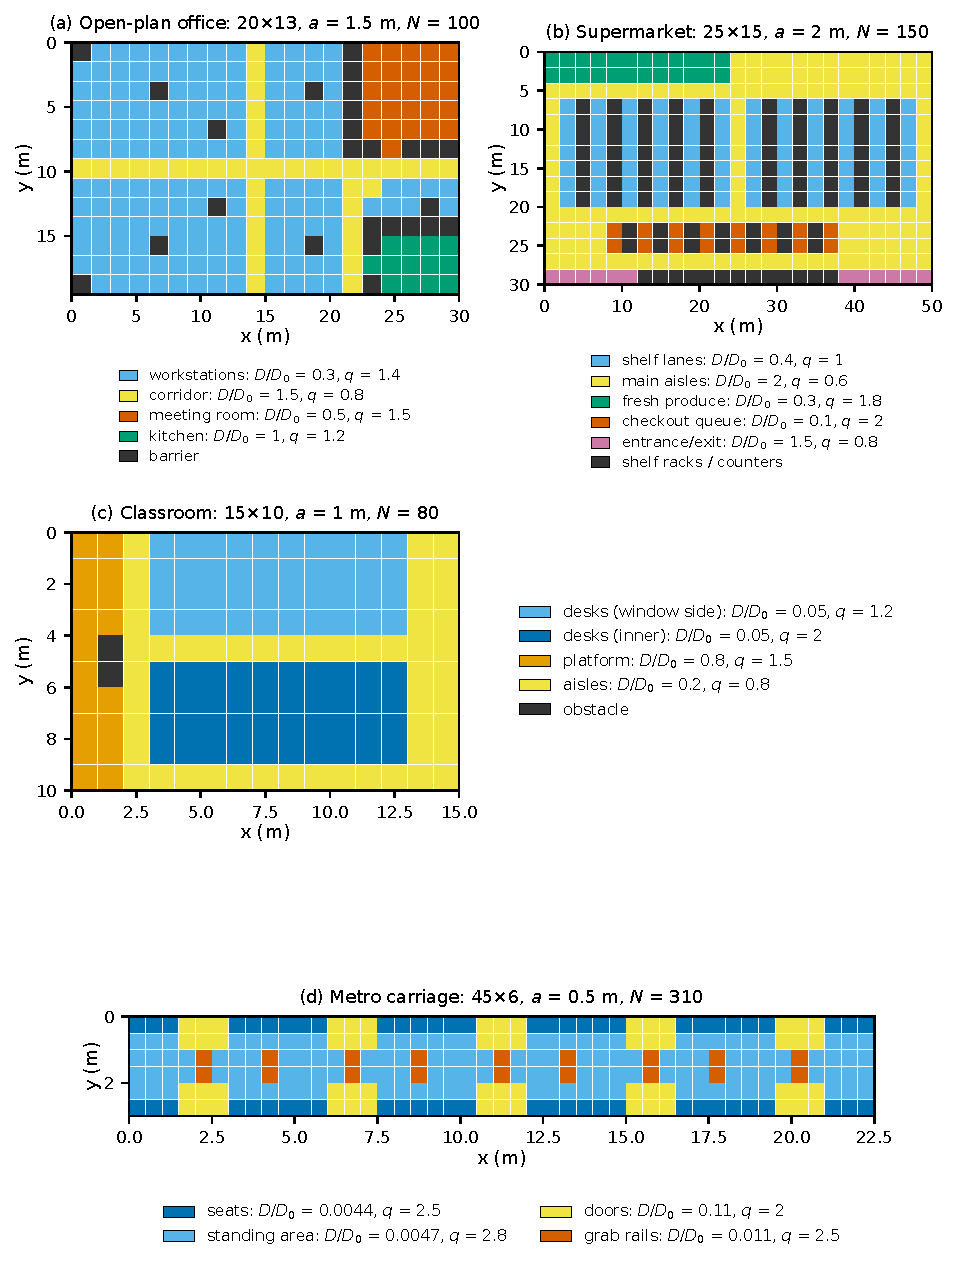
\includegraphics[width=0.84\textwidth]{fig3_scene_maps_en}
\caption{Floor plans of the four scenes. Each small square is one lattice cell of side $a$; colours mark
the zones, whose mobility multiplier $D/\Dz$ and infection efficiency $q$ are given in the legends; dark
cells are barriers and are not part of $\cells$. The panel titles give the lattice size in cells, the
spacing $a$ and the number of people $\Npop$. The arrangement of the zones and the zone values are
illustrative assumptions (see text).}
% src: figures/fig3_scene_maps_{en,zh}.pdf, script code/bsc_sim/experiments/20_figures.py (fig_scenes), scenes code/bsc_sim/scenes/*.json
\label{s2_model:fig:scenes}
\end{figure}

The model is evaluated on four scenes: an open-plan office, a supermarket, a classroom and a metro carriage
(Table~\ref{s2_model:tab:scenes}, Fig.~\ref{s2_model:fig:scenes}). The same scene files are used for the
theory and for the simulations. The lattice sizes and spacings, the zones with their values of $d$ and $q$,
the numbers of people and the arrangement of the zones on the floor are illustrative assumptions; they are not
measurements and are not derived from any standard. In the office the zones cover 60, 15, 10, 5 and 10\,\% of
the 260 cells of the floor (workstations, corridor, meeting room, kitchen and barriers; the 234 walkable cells
exclude the barriers); in the supermarket shelf racks and
counters act as barriers; the classroom desks are split into a window block ($q=1.2$) and an inner block
($q=2.0$); and the carriage has doors, seats and grab rails.
% src: code/bsc_sim/scenes/office.json (zone_counts 156, 39, 26, 13, 26 of 260 cells); code/bsc_sim/scenes/supermarket.json, classroom.json, metro.json
The metro mobilities follow a crowding rule $d=c\,n_{\mathrm{d}}^{-\eta}$ with $\eta=2$ in the standing area
and $\eta=1$ elsewhere, evaluated at the crowd density $n_{\mathrm{d}}=310/67.5\,\mathrm{m}^2=4.59$ people per
$\mathrm{m}^2$; their area
mean is $0.028$.
% src: data/s2_model_scenes.json -> scenes.metro (density_used_for_metro_rule_per_m2 4.5926, d_mean 0.0282, zones); code/bsc_sim/scenes/metro.json (D_coef, D_exp)
The quantity that enters the bounds of Section~\ref{s3_r0:sec} is the mean of $q$ over walkable cells, which
is $1.300$, $0.914$, $1.318$ and $2.536$. The 1\,m kernel is the same-cell kernel in the office and the
supermarket; it contains the cell and up to four neighbours in the classroom ($4.6$ cells on average) and up
to 13 cells in the carriage ($11.1$ on average). Results for the same-cell kernel in these two scenes are
reported alongside as a sensitivity case.
% src: data/s2_model_scenes.json -> scenes.<name>.q_mean; scenes.<name>.kernel1m_cells_mean (1.0, 1.0, 4.62, 11.13), kernel1m_cells_max (1, 1, 5, 13)

\subsection{Parameters and physical regime}\label{s2_model:sec:regime}

The default epidemiological parameters are $\beta=0.5\perday$ and $\gamma=0.14\perday$, a mean infectious
period of $7.1$ days and $\beta/\gamma=3.571$. They are illustrative values and are not calibrated to any
disease or dataset. The same holds for the default mobility scale $\Dz=1\cellday$, and this value matters
for every result below. It is used as a reference low-mobility value at which the spatial effects of the model
are visible; most results are also given at $\Dz=10$ and
$100\cellday$, and $\Rz$ of every scene at walking mobility (Table~\ref{s2_model:tab:regime}).
% src: data/s2_model_scenes.json -> beta, gamma, beta_over_gamma (3.5714), office_regime.infectious_period_days (7.14)

\paragraph{What $\Dz=1$ means.} In the office ($a=1.5$\,m), $\Dz=1\cellday$ is $2.25\,\mathrm{m}^2$ per day.
The root-mean-square displacement $\sqrt{4Dt}$ of a walker with $d=1$ is then $3$\,m in a day and $8$\,m in a
mean infectious period, in a room of $30\,\mathrm{m}\times19.5\,\mathrm{m}$. A walker in the meeting room of
this scene (26 cells) leaves it at the principal rate $\muZ=0.00877\perday$: its residence time $1/\muZ$ is
$114$ days, sixteen infectious periods. In the metro carriage at $\Dz=1$ a passenger makes on average $0.075$
hops of $0.5$\,m per day: the carriage is frozen on the time scale of an infectious period.
% src: data/s2_model_scenes.json -> office_regime (D0_m2_per_day 2.25, rms_m_per_day_D0 3.0, rms_m_per_infectious_period_D0 8.02), scenes.office.floor_m
% src: data/s2_model_scenes.json -> office_regime (meeting_room_mu_Z_per_day 0.008769, meeting_room_1_over_mu_Z_days 114.04)
% src: data/s2_model_scenes.json -> scenes.metro.hop_rate_mean_per_day_D0=1 (0.0749)

\paragraph{Walking mobility.} For a walker whose velocity autocorrelation decays as
$\langle\mathbf{v}(0)\cdot\mathbf{v}(t)\rangle=v^2\e^{-t/\tau}$, the diffusion coefficient in two dimensions
is $D=\tfrac12\int_0^\infty\langle\mathbf{v}(0)\cdot\mathbf{v}(t)\rangle\,\dd t=v^2\tau/2$
\citep{taylor1922diffusion,kubo1966fluctuation}. With an assumed walking speed $v=1.3\,\mathrm{m\,s^{-1}}$, a
typical value for pedestrians \citep{weidmann1993transporttechnik}, and an assumed persistence time
$\tau=1.5$\,s, this gives $D=1.27\,\mathrm{m^2\,s^{-1}}$, that is, $4.9\times10^{4}\cellday$ for $a=1.5$\,m,
and $2.4\times10^{3}\cellday$ if people walk 5\,\% of the time. Over the four scenes these walking values lie
between $1.4\times10^{3}$ and $4.4\times10^{5}\cellday$ (Table~\ref{s2_model:tab:regime}): $\Dz=1$ is three to
almost six orders of magnitude below the mobility of people who walk.
% src: data/s2_model_scenes.json -> walking (D_m2_per_s 1.2675), scenes.office (walking_D0_cell2_per_day 48672, walking_5pct_D0_cell2_per_day 2433.6); same values in data/bsc_theory/worked_examples.json -> E9_physical_D
% src: data/s2_model_scenes.json -> scenes.<name>.walking_5pct_D0_cell2_per_day (smallest: supermarket 1368.9), walking_D0_cell2_per_day (largest: metro 438048); log10: 3.14 to 5.64 (data/misc_checks.json -> mobility_gap)

\begin{table}[tbp]
\centering
\caption{Basic reproduction number $\Rz$ of the mean-field model ($\beta=0.5\perday$,
$\gamma=0.14\perday$) for the mobility scales $\Dz$ (in \cdunit) used in this article and for walking
mobility; in brackets and in the columns headed `excess', the excess of $\Rz$ over the well-mixed value
$\beta\langle q\rangle/\gamma$ in per cent. For the office and the supermarket the 1\,m kernel is the
same-cell kernel; for the classroom and the metro carriage both kernels are given.
The walking values of $\Dz$ are $v^2\tau/2$ with $v=1.3\,\mathrm{m\,s^{-1}}$ and $\tau=1.5$\,s, converted
with the lattice spacing of each scene, for people who walk 5\pct{} of the time and all the time.}
\label{s2_model:tab:regime}
\footnotesize
% src: data/s2_model_scenes.json -> scenes.<name>.R0_1m, scenes.<name>.R0_samecell (rows as generated in
%      data/s2_model_table_rows.tex); D0 = 1, 10, 100 agree with data/plan_theory_checks.json ->
%      scenes.<name>.R0_1m_D0=*, R0_samecell_D0=*
\setlength{\tabcolsep}{3pt}
\begin{tabular}{@{}llcccccccc@{}}
\toprule
 & & & \multicolumn{3}{c}{$\Rz$ (excess, \%) at $\Dz=$}
 & \multicolumn{2}{c}{walking 5\pct} & \multicolumn{2}{c}{walking} \\
\cmidrule(lr){4-6}\cmidrule(lr){7-8}\cmidrule(l){9-10}
Scene & kernel & $\beta\langle q\rangle/\gamma$ & 1 & 10 & 100 & $\Dz$ & excess & $\Dz$ & excess \\
\midrule
Office & same cell & 4.643 & 5.107 (10.0) & 4.676 (0.72) & 4.646 (0.06) & $2.4\times10^{3}$ & 0.0026 & $4.9\times10^{4}$ & 0.00013 \\
Supermarket & same cell & 3.263 & 4.394 (34.6) & 3.391 (3.93) & 3.275 (0.37) & $1.4\times10^{3}$ & 0.0268 & $2.7\times10^{4}$ & 0.00134 \\
Classroom & 1\,m & 4.706 & 5.866 (24.7) & 4.931 (4.79) & 4.731 (0.53) & $5.5\times10^{3}$ & 0.0098 & $1.1\times10^{5}$ & 0.00049 \\
 & same cell &  & 6.182 (31.4) & 4.960 (5.42) & 4.733 (0.57) & $5.5\times10^{3}$ & 0.0105 & $1.1\times10^{5}$ & 0.00053 \\
Metro carriage & 1\,m & 9.056 & 9.241 (2.1) & 9.164 (1.20) & 9.078 (0.25) & $2.2\times10^{4}$ & 0.0013 & $4.4\times10^{5}$ & 0.00006 \\
 & same cell &  & 9.836 (8.6) & 9.308 (2.79) & 9.086 (0.33) & $2.2\times10^{4}$ & 0.0016 & $4.4\times10^{5}$ & 0.00008 \\
\bottomrule
\end{tabular}
\end{table}

\paragraph{Consequence.} At $\Dz=1$ the heterogeneity of $q$ raises $\Rz$ above the well-mixed value
$\beta\langle q\rangle/\gamma$ by $2$ to $35\pct$ (1\,m kernel), depending on the scene. At walking mobility
the excess is below $0.003\pct$ in the office and below $0.03\pct$ in every scene: in the mean-field model a
closed room in which people walk is well mixed, and $\Rz=\beta\langle q\rangle/\gamma$ for all practical
purposes.
% src: data/s2_model_scenes.json -> scenes.<name>.R0_1m.*.excess_over_wellmixed_pct (D0=1: 10.0, 34.6, 24.7, 2.05;
%      walking_5pct: 0.0026, 0.0268, 0.0098, 0.0013; walking: 0.00013, 0.00134, 0.00049, 0.00006);
%      office at D0 = 2400 and 48700 in data/plan_theory_checks.json -> office.mobility_table (0.0027, 0.00013)
All spatial effects in closed rooms reported in Sections~\ref{s3_r0:sec}--\ref{s6_scenes:sec} are large only at
low mobility, and this holds for the pair-level correction of Section~\ref{s5_pair:sec} as well. Leaks through
a localised door are the exception: their effect grows with mobility (Section~\ref{s4_geometry:sec:leaky}).
Results are therefore given for the low default $\Dz=1$ and for $\Dz=10$ and $100$, where the room approaches
the well-mixed limit; the later sections refer back to this paragraph and do not repeat it. A small $\Dz$
could be read as a stand-in for people who stay at a desk or a seat, but a random walk without home positions
is not an adequate model of such people: a slow walker drifts away and does not return, and the stationary
occupancy is uniform over all walkable cells, corridors and aisles included. Section~\ref{s8b_evidence:sec:contacts}
shows the consequence against recorded contacts, at the mobility that matches recorded contact durations: a
free walk calibrated to the amount and duration of contact in six indoor settings gives each person too many
partners in five of the six settings and no group structure in any.

\paragraph{Closed room.} Unless stated otherwise, each scene is a closed room occupied 24 hours a day by the
same $\Npop$ people for the whole epidemic. This is an idealisation for the office and the classroom, and it
is not a physical scenario for the supermarket and the metro carriage, for which the scene files assume visits
of 27 and 20 minutes;
% src: code/bsc_sim/scenes/supermarket.json, metro.json ("dwell")
Section~\ref{s6_scenes:sec:interventions} gives the corresponding numbers per visit and for a room that is
occupied during part of the day.

% m3_r0.tex -- Main text, Section 3: the basic reproduction number of the mean-field model.
% Proofs are in the Supplementary Material (supp_r0.tex); they follow code/bsc_theory/scripts and the
% derivations checked there, in the article's notation (cells x, y; column index = source cell).
% Numbers: data/plan_theory_checks.json (canonical scenes; code/plan_theory_checks.py) and
% data/s3_r0_checks.json (written by code/s3_r0_checks.py, which recomputes them with
% other code and agrees with the first file to 2e-14).
% Paths in "% src:" comments are relative to the repository root.
\section{The basic reproduction number of the mean-field model}\label{s3_r0:sec}

This section determines the basic reproduction number $\Rz$ of the mean-field model
\eqref{s2_model:eq:meanfield}, its bounds and its dependence on mobility. Throughout, Assumption~\ref{s2_model:ass:A}
holds, $\Vm=\gamma\Id-\gen$, the column index of a matrix is the source cell, and inequalities between vectors
or matrices are entrywise. Each statement names the contact kernel it needs: most require the same-cell
kernel, $\Fm=\beta\Qm$, with $q\ge0$, $q\not\equiv0$. The main results are known for epidemic patch models
(Section~\ref{s1_intro:sec}, Table~\ref{s1_intro:tab:known}), and no novelty is claimed for them. Complete proofs
from standard facts on non-negative matrices are given in Supplementary Section~\ref{S-appS_r0:sec}, because
they fix the conditions under which each statement holds (which kernel, which symmetry of the hop rates). The
zone bound, the slow-mixing coefficient and the edge-wise monotonicity are elementary consequences of the same
matrix theory; a targeted search (Crossref queries on patch-model reproduction numbers and dispersal,
1~October 2026) found no source for them, which does not establish that there is none.
% src: data/refs_search.json (searches; manual_checks: gao2020fast, tien2015disease, allen2007asymptotic)

\begin{theorem}[Next-generation matrix]\label{s3_r0:thm:ngm}
  Let Assumption~\ref{s2_model:ass:A} hold, let $\Fm\ge0$, $\Fm\neq0$, $\Vm=\gamma\Id-\gen$, and define
  \begin{equation}\label{s3_r0:eq:ngm}
     \ngm=\Fm\Vm^{-1},\qquad \Rz=\srad(\ngm),\qquad \lamone=\sabs(\Jm),\quad \Jm=\gen+\Fm-\gamma\Id .
  \end{equation}
  \begin{enumerate}[label=\textup{(\alph*)},leftmargin=*]
    \item $\Vm^{-1}=\int_0^\infty \e^{-\gamma t}\e^{\gen t}\,\dd t>0$ entrywise.  For $\Fm=\beta\ker^{\T}\Qm$,
      $K_{yx}=\beta\sum_{z}P_{zy}\,q_z\int_0^\infty \e^{-\gamma t}P_t(z\,|\,x)\,\dd t$ is the expected number of
      infections generated in cell $y$ by one infective introduced in cell $x$ of a fully susceptible room;
      for the same-cell kernel, $K_{yx}=\beta q_y\int_0^\infty \e^{-\gamma t}P_t(y\,|\,x)\,\dd t$.
    \item $\Rz>0$, and $\Rz$ is the unique $R>0$ with $\sabs(\gen+\Fm/R-\gamma\Id)=0$.
    \item $\lamone<0\iff\Rz<1$, $\lamone=0\iff\Rz=1$, $\lamone>0\iff\Rz>1$.
    \item Every solution of \eqref{s2_model:eq:meanfield} satisfies $I(t)\le \e^{\Jm t}I(0)$ componentwise
      for all $t\ge0$.  Hence if $\Rz<1$ the infective population is bounded by a decaying exponential from
      $t=0$ on, $\one^{\T}I(t)\le C\,\e^{\lamone t}\,\one^{\T}I(0)$ with $\lamone<0$ and $C$ independent of the
      initial condition.  If $\Rz>1$ the disease-free state is unstable and the linearised solution grows like
      $\e^{\lamone t}$.
  \end{enumerate}
\end{theorem}

In a closed SIR model the infectives vanish for every value of $\Rz$; the content of (d) is that for $\Rz<1$
there is no growth at any time, whereas for $\Rz>1$ a small seed grows until the depletion of susceptibles
stops it. The column sums of $\ngm$ are the expected numbers of secondary cases of an index case introduced in
cell $x$, the offspring number $\noff(x)$; for every row-stochastic kernel
\begin{equation}\label{s3_r0:eq:offspring}
  \noff(x)=\sum_yK_{yx}=\beta\,\Exp_x\!\int_0^{\tau}q(X_t)\,\dd t ,\qquad
  \frac{\beta\qmin}{\gamma}\le\noff(x)\le\frac{\beta\qmax}{\gamma},\qquad \sum_x\pi_x\noff(x)=\frac{\beta\qmean}{\gamma},
\end{equation}
where $X_t$ is the walk started at $x$ and $\tau$ its exponential infectious period. In the office scene at
$\Dz=1\cellday$, $\noff(x)$ ranges from $3.995$ to $5.335$ over the cells, with uniform mean $4.643$.
% src: data/plan_theory_checks.json: office/D0=1/offspring_min, offspring_max, offspring_uniform_mean
The next-generation matrix is $\ngm=\Fm\,\widehat G(\gamma)$, where $\widehat G(\gamma)=(\gamma\Id-\gen)^{-1}$ is the Laplace transform of the
lattice propagator at the recovery rate; for reversible movement $\Rz$ also has a variational (Rayleigh) form
and a modal matrix form in the eigenmodes of the movement generator, whose largest diagonal entry is only a lower
bound (Supplementary Theorem~\ref{S-s3_r0:thm:rayleigh} and Corollary~\ref{S-s3_r0:cor:modal}).

\begin{theorem}[Bounds; same-cell kernel]\label{s3_r0:thm:bounds}
  Let Assumption~\ref{s2_model:ass:A} hold and $\Fm=\beta\Qm$ with $q\ge0$, $q\not\equiv0$.  Then, for every
  irreducible generator (reversible or not),
  \begin{equation}\label{s3_r0:eq:bounds}
    \frac{\beta\qmean}{\gamma}\le\Rz\le\frac{\beta\qmax}{\gamma},\qquad
    \beta\qmean-\gamma\le\lamone\le\beta\qmax-\gamma .
  \end{equation}
  If $q$ is constant all four are equalities; if $q$ is not constant all four inequalities are strict.
\end{theorem}

By \eqref{s3_r0:eq:offspring}, $\beta\qmean/\gamma$ is the mean number of secondary cases of an index case
placed according to the stationary distribution. $\Rz$ is larger because secondary cases are not born at
stationarity: they are born preferentially in cells of high $q$ and begin their infectious period there.
Mobility erases this memory of the birthplace (Theorem~\ref{s3_r0:thm:mobility}). With the same-cell kernel
there is therefore no mechanism by which spatial separation could lower the mean-field $\Rz$ below the
well-mixed value $\beta\qmean/\gamma$; what separation does to discrete individuals is a different question
(Sections~\ref{s5_pair:sec} and~\ref{s6_scenes:sec}).

\begin{theorem}[Mobility; same-cell kernel]\label{s3_r0:thm:mobility}
  Let $\gen=\Dz\genz$ with $\genz$ an irreducible generator with stationary distribution $\stat$, and
  $\Fm=\beta\Qm$.  Then
  \begin{enumerate}[label=\textup{(\alph*)},leftmargin=*]
    \item $\lim_{\Dz\to\infty}\Rz(\Dz)=\beta\qmean/\gamma$;
    \item $\lim_{\Dz\to0^+}\Rz(\Dz)=\beta\qmax/\gamma$;
    \item $\lamone(\Dz)$ is convex and non-increasing, and $\Rz(\Dz)$ is non-increasing; if $q$ is not constant,
      $\Rz(\Dz)$ is strictly decreasing on $(0,\infty)$.
  \end{enumerate}
  No reversibility is needed.
\end{theorem}

\begin{proposition}[Expansions]\label{s3_r0:prop:expansions}
  In the setting of Theorem~\ref{s3_r0:thm:mobility}:
  \begin{enumerate}[label=\textup{(\roman*)},leftmargin=*]
    \item as $\Dz\to\infty$, $\Rz(\Dz)=\dfrac{\beta\qmean}{\gamma}+\dfrac{\beta\,C}{\qmean\,\Dz}+O(\Dz^{-2})$, where
      $C=\qvec^{\T}\mathbf{y}\ge0$ and $\mathbf{y}$ solves $-\genz\mathbf{y}=\Qm\stat-\qmean\stat$, $\one^{\T}\mathbf{y}=0$
      (for symmetric rates, $C=\ncell^{-1}\,\delta q^{\T}(-\genz)^{+}\delta q$ with $\delta q=\qvec-\langle q\rangle\one$
      and $(\cdot)^{+}$ the pseudo-inverse);
    \item as $\Dz\to0$, $\Rz(\Dz)=\dfrac{\beta\qmax}{\gamma}\Bigl(1-\dfrac{\Dz\,\mu^0_Z}{\gamma}\Bigr)+o(\Dz)$, where
      $Z=\{x:q_x=\qmax\}$ and $\mu^0_Z=-\sabs(\genz[Z,Z])$.
  \end{enumerate}
\end{proposition}

\begin{proposition}[Zone bound]\label{s3_r0:prop:zone}
  Let Assumption~\ref{s2_model:ass:A} hold and $\Fm=\beta\Qm$.  For every non-empty $Z\subset\cells$,
  \begin{equation}\label{s3_r0:eq:zone}
    \Rz\ \ge\ \frac{\beta\,q_Z}{\gamma+\muZ},\qquad q_Z=\min_{x\in Z}q_x,\qquad \muZ=-\sabs(\gen[Z,Z])\ge0 .
  \end{equation}
\end{proposition}

Here $\muZ$ is the principal decay rate of a walker that is killed when it steps out of $Z$. By
Proposition~\ref{s3_r0:prop:expansions}(ii) the zone bound with $Z=\{x:q_x=\qmax\}$ is sharp to first order as
$\Dz\to0$. An expression of the form $\beta q/(\gamma+\mu)$ thus does occur in the closed room, but as a lower
bound contributed by a high-risk zone from which infectives escape into lower-risk space, with $q$ and $\mu$
those of the zone and not of the room.

\begin{theorem}[Edge-wise monotonicity; symmetric rates, same-cell kernel]\label{s3_r0:thm:edges}
  If $\hop{x}{y}=\hop{y}{x}$ for all edges and $\Fm=\beta\Qm$, then $\Rz$ and $\lamone$ are non-increasing
  functions of each individual edge rate.  Consequently, under rule \eqref{s2_model:eq:hop} and for a fixed set
  of cells $\cells$, lowering $D$ in any set of cells or closing edges (walls between cells) cannot lower $\Rz$.
\end{theorem}

The theorem concerns operations that keep the set of cells. Turning cells into barrier cells removes them, and
their $q$, from $\cells$; this changes $\qmean$ and both bounds of Theorem~\ref{s3_r0:thm:bounds}, and $\Rz$ can
then fall (Section~\ref{s4_geometry:sec:examples}). The symmetry is essential: under a departure-site rule a
change of $D$ also changes the stationary occupancy, and in $300$ random instances multiplying $D$ by $3$ in
one cell raised $\Rz$ in $201$, lowered it in $98$ and left it unchanged (to $10^{-10}$) in one.
% src: data/bsc_theory/verify_theorems.json: T3p/departure_up, departure_down

\begin{proposition}[Contact kernels]\label{s3_r0:prop:kernel}
  Let $\Fm=\beta\ker^{\T}\Qm$ with $\ker$ row-stochastic.  Then
  \begin{enumerate}[label=\textup{(\roman*)},leftmargin=*]
    \item Theorem~\ref{s3_r0:thm:ngm} holds;
    \item $\beta\qmin/\gamma\le\Rz\le\beta\qmax/\gamma$, and $\Rz=\beta q_0/\gamma$ if $q\equiv q_0$;
    \item $\Rz(\Dz)\to\beta\qmean/\gamma$ as $\Dz\to\infty$ and $\Rz(\Dz)\to\srad(\beta\ker^{\T}\Qm)/\gamma$ as $\Dz\to0$;
    \item the lower bound $\beta\qmean/\gamma\le\Rz$ of Theorem~\ref{s3_r0:thm:bounds} and the monotonicity of
      Theorem~\ref{s3_r0:thm:mobility}(c) can fail.  Example: three cells in a row, hop rate $\Dz$ between neighbours,
      $\ker$ uniform over a cell and its neighbours, $q=(1,0,1)$: then
      $\Rz(\Dz)=(\beta/\gamma)(\gamma+4\Dz)/(2\gamma+6\Dz)$, which is $0.5\,\beta/\gamma$ at $\Dz=0$,
      below $\beta\langle q\rangle/\gamma=0.667\,\beta/\gamma$, and increases with $\Dz$.
  \end{enumerate}
\end{proposition}
% src: data/plan_theory_checks.json: checks/kernel_counterexample_q=[1.0, 0.0, 1.0] (0.500, 0.503, 0.529,
%      0.614, 0.659, 0.666, 0.6667 at D0 = 0, 0.001, 0.01, 0.1, 1, 10, 1000 with gamma = 0.14);
%      closed form checked to 8e-14 in data/s3_r0_checks.json: kernel_closed_form_max_abs_diff

With a contact kernel, an infective in a high-$q$ cell infects people in neighbouring cells; if those cells
have low $q$ and nobody moves, the new cases transmit little, and the size bias that raises $\Rz$ for the
same-cell kernel is reversed. In the two scenes in which the 1\,m kernel differs from the same-cell kernel the
lower bound happens to hold ($5.866\ge4.706$ in the classroom and $9.241\ge9.056$ in the metro carriage at
$\Dz=1\cellday$), but it is not guaranteed.
% src: data/plan_theory_checks.json: scenes/classroom, scenes/metro (R0_1m_D0=1, lower)

\subsection{The scenes}\label{s3_r0:sec:scenes}

\begin{figure}[tbp]
  \centering
  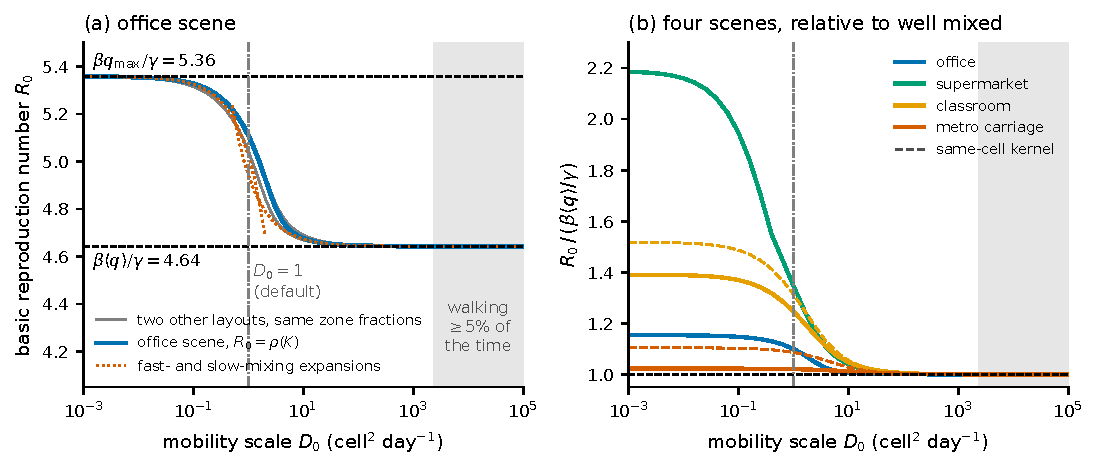
\includegraphics[width=\textwidth]{fig_r0_mobility_en}
  \caption{Mean-field basic reproduction number $\Rz=\srad(\ngm)$ against the mobility scale $\Dz$
  (\cdunit), for $\beta=0.5\perday$ and $\gamma=0.14\perday$; $\Rz$ does not depend on the number of
  people $\Npop$ (frequency-dependent incidence), and no simulation is involved.
  (a)~Office scene (234 walkable cells, same-cell kernel): $\Rz$ (thick line), the bounds
  $\beta\langle q\rangle/\gamma$ and $\beta\qmax/\gamma$ of Theorem~\ref{s3_r0:thm:bounds} (dashed), the two
  expansions of Proposition~\ref{s3_r0:prop:expansions} (dotted), and two other floor plans with the same zone
  fractions (thin grey).  (b)~The four scenes, as the ratio of $\Rz$ to the well-mixed value
  $\beta\langle q\rangle/\gamma$, with the 1\,m contact kernel (solid) and the same-cell kernel (dashed; the
  two coincide for the office and the supermarket).  The dash-dotted vertical line marks the default
  $\Dz=1$; the shaded band is $\Dz\ge2.4\times10^{3}$, which for the lattice spacing of the
  office ($a=1.5$\,m) is the mobility of people who walk at least 5\pct{} of the time
  (Section~\ref{s2_model:sec:regime}; the values for the other scenes are in Table~\ref{s2_model:tab:regime}).}
  % src: code/plan_fig_theory.py (fig_r0_mobility) <- data/plan_theory_checks.json, plan_theory_sweeps.npz
  \label{s3_r0:fig:mobility}
\end{figure}

For every floor plan with the zone fractions of the office scene ($\langle q\rangle=1.300$, $\qmax=1.5$),
Theorem~\ref{s3_r0:thm:bounds} gives $4.643\le\Rz\le5.357$. In the scene itself $\Rz=5.107$ at
$\Dz=1\cellday$, with growth rate $\lamone=0.602\perday$ (doubling time $1.15$ days); two other floor plans
with the same zone fractions give $5.109$ and $5.041$.
% src: data/plan_theory_checks.json: office/lower_bound, upper_bound, q_mean, q_max
% src: data/plan_theory_checks.json: office/D0=1 (R0, lambda1, doubling_time); alternative_layouts/O1, O2 (R0_D0_1)
The curve $\Rz(\Dz)$ decreases from the upper to the lower bound (Fig.~\ref{s3_r0:fig:mobility}a), and the
two expansions of Proposition~\ref{s3_r0:prop:expansions} are $\Rz\simeq4.643+0.296/\Dz$ as $\Dz\to\infty$
and $\Rz\simeq5.357\,(1-0.0626\,\Dz)$ as $\Dz\to0$ ($\Dz$ in \cdunit). The first is accurate to $0.004$ at
$\Dz=10$ and to $3\times10^{-5}$ at $\Dz=100$, the second to $0.003$ at $\Dz=0.1$.
% src: data/plan_theory_checks.json: office/largeD_coefficient_betaC_over_qbar, office/smallD_slope_muZ0_over_gamma
% src: data/s3_r0_checks.json: office/expansions/rows (err_fast, err_slow)
The set $Z$ of the slow-mixing expansion is the meeting room (26 cells, $q=1.5$), whose quasi-stationary
residence time at $\Dz=1$ is $1/\muZ=114$ days; its zone bound \eqref{s3_r0:eq:zone} is $5.041$. These are
properties of this floor plan, in which the meeting room is connected to the corridor through a single cell.
% src: data/plan_theory_checks.json: office/zone_bound_meeting_room (mu_Z, exit_time_days, bound, cells)
Over the four scenes the excess of $\Rz$ over the well-mixed value at $\Dz=1$ is largest in the supermarket
($+34.6\pct$), where $\qmax$ is more than twice $\langle q\rangle$ (Table~\ref{s2_model:tab:regime},
Fig.~\ref{s3_r0:fig:mobility}b).
% src: data/s3_r0_checks.json: scenes/supermarket/D0=1/excess_1m_pct

For a two-zone room, a workspace ($q_W=1.5$, $D=0.3\,\Dz$) and a central corridor band ($q_C=0.5$,
$D=2\,\Dz$) on a $20\times13$ lattice with $\langle q\rangle=1.2$, Theorem~\ref{s3_r0:thm:bounds} gives
$\Rz\ge1.2\,\beta/\gamma$: separating a low-risk corridor from a high-risk workspace cannot lower the
mean-field $\Rz$. Numerically $\Rz=4.972=1.39\,\beta/\gamma$ at $\Dz=1$, $1.24\,\beta/\gamma$ at $\Dz=10$ and
$1.20\,\beta/\gamma$ for $\Dz\ge100$. Four other arrangements of the same two zones, with $69$--$70\pct$
workspace, give $1.43\,\beta/\gamma$ (corridor band along one wall) and $1.22$--$1.23\,\beta/\gamma$ (aisles, a
grid of aisles, scattered corridor cells) at $\Dz=1$: the finer the two zones are interleaved, the closer $\Rz$
is to the well-mixed value.
% src: data/bsc_sim/05_heterogeneity.json: "D0=1|N=100|c=0.5833"/R0_ngm = 4.972; data/s3_r0_checks.json: two_zone/rows (1.3922, 1.2395, 1.2043, 1.2004)
% src: data/bsc_theory/worked_examples.json: E1_two_zone/{side,aisles,grid,scatter}/symmetric/R0_over_beta_gamma
%      (1.425, 1.224, 1.221, 1.227; workspace 180/260 or 182/260 cells)

Every statement of this section was tested on random instances of four families of generators, and the proofs
were re-derived and the computations re-implemented in the re-check (Supplementary
Section~\ref{S-appA_numerics:sec:theorems}); over $2{,}000$ random instances, for example, the largest violation
of the bounds \eqref{s3_r0:eq:bounds} was $4\times10^{-14}$, at the level of rounding error.
% src: data/bsc_theory/verify_theorems.json: T2 (n_instances 2000, max_viol_upper 4.0e-14, max_viol_lower 2.3e-15)

% m4_geometry.tex -- Main text, Section 4: Room size, leaks and hotspot maps.
% Paths in "% src:" comments are relative to the repository root.
% Numbers come from  data/plan_theory_checks.json (canonical office scene, written by
% code/plan_theory_checks.py),  data/bsc_theory/worked_examples.json and
% fig2_room_size_data.json (room size, leaks; written by code/bsc_theory/scripts/worked_examples.py
% and make_figures.py),  data/s4_geometry_checks.json (derived numbers and a second computation;
% written by code/s4_geometry_checks.py), data/s4_geometry_barriers_leak.json and
% data/s4_geometry_leak_kernels.json.  Proofs: Supplementary Section S3.
\section{Room size, leaks and hotspot maps}\label{s4_geometry:sec}

Section~\ref{s3_r0:sec} showed that mobility and the heterogeneity of $q$ together place $\Rz$ between
$\beta\qmean/\gamma$ and $\beta\qmax/\gamma$. This section asks what the geometry of the room adds. None of it
is claimed as new: the invariance of Theorem~\ref{s4_geometry:thm:closed} is known for patch models whose
patches have equal reproduction numbers \citep{gao2011sis}; loss through an absorbing boundary is the
critical-patch-size mechanism of Skellam \citep{skellam1951random,cantrell2003spatial}; the quasi-stationary
objects of Theorem~\ref{s4_geometry:thm:leaky} go back to \citet{darroch1967quasi}; and
Theorem~\ref{s4_geometry:thm:hotspots} is Perron--Frobenius theory together with the sensitivity of a simple
eigenvalue \citep{berman1994nonnegative,horn2013matrix}. For the leaky-room formulation as stated here we know
of no source; we searched only for the patch-model results of Section~\ref{s1_intro:sec}. Proofs are in
Supplementary Section~\ref{S-appS_geometry:sec}.

\subsection{Closed rooms: no finite-size effect}\label{s4_geometry:sec:closed}

\begin{theorem}[Closed room, uniform $q$]\label{s4_geometry:thm:closed}
  Let Assumption~\ref{s2_model:ass:A} hold, $q\equiv q_0$ and $\Fm=\beta\ker^{\T}\Qm$ with any row-stochastic
  kernel. Then $\Rz=\beta q_0/\gamma$ and $\lamone=\beta q_0-\gamma$ for every room size, shape, barrier
  layout, mobility field and mobility scale, and every index case causes $\noff(x)=\beta q_0/\gamma$ secondary
  cases in expectation in the mean-field model, wherever it starts.
\end{theorem}

Reflecting walls lose nobody: all column sums of $\ngm$ equal $\beta q_0/\gamma$. Equivalently, for uniform $q$
the modal matrix of Supplementary Corollary~\ref{S-s3_r0:cor:modal} is diagonal with entries
$\beta q_0/(\gamma+\mu_j)$, and the largest is the entry of the uniform mode, $\mu_0=0$; the first non-zero
eigenvalue $\mu_1=2D[1-\cos(\pi/L)]\approx\pi^2D/L^2$ of a square room of side $L$ (cells) plays no role. Square rooms with $L=3,\dots,40$ and
$D=0.5\cellday$ give $\srad(\ngm)=\beta q/\gamma$ to within $6\times10^{-15}$ in relative terms, and forty
random rooms with barrier cells, mobilities spread over four decades, symmetric and non-symmetric generators
and random contact kernels reproduce $\Rz=\beta q_0/\gamma$, $\lamone=\beta q_0-\gamma$ and
$\noff(x)=\beta q_0/\gamma$ to within $10^{-13}$. In a closed room, geometry therefore enters $\Rz$ only through
the interplay of mobility with the heterogeneity of $q$.
% src: data/bsc_theory/fig2_room_size_data.json (refl: max |ratio-1| = 5.8e-15);
% src: data/s4_geometry_checks.json: B_closed_room_general_kernel (1.9e-14, 1.8e-14, 6.5e-14)

\subsection{Leaky rooms}\label{s4_geometry:sec:leaky}

A genuine boundary effect requires that people leave. Suppose that a person in cell $x$ leaves the room at
rate $\kappa_x\ge0$ (through a door cell, an open side, or after a dwell time that does not depend on
position) and is replaced at once by a susceptible person entering through the same cell, so that the
occupancy stays at $N^*$; only infections that take place inside the room are counted. An infective then
follows the killed walk with generator $\genk=\gen-\diag\kappa$.

\begin{theorem}[Leaky room; same-cell kernel]\label{s4_geometry:thm:leaky}
  Let Assumption~\ref{s2_model:ass:A} hold, $\Fm=\beta\Qm$, $\kappa\ge0$, $\kappa\not\equiv0$, and put
  $\genk=\gen-\diag\kappa$, $\Vm_\kappa=\gamma\Id-\genk$, $\Rroom=\srad(\beta\Qm\Vm_\kappa^{-1})$ and
  $\muk=-\sabs(\genk)$. Let $\uvec_\kappa,\lvec_\kappa>0$ be the right and left Perron vectors of $\genk$ and
  $\nu=(\lvec_\kappa\circ\uvec_\kappa)/(\lvec_\kappa^{\T}\uvec_\kappa)$. Then
  \begin{enumerate}
    \item[(1)] Theorem~\ref{s3_r0:thm:ngm}(a)--(c) holds with $\gen$ replaced by $\genk$;
    \item[(2)] $0<\muk\le\langle\kappa\rangle_\pi:=\sum_x\pi_x\kappa_x$; $\muk$ is non-decreasing in every
       $\kappa_x$; and for
       $\kappa=k\,\one_\Delta$ with a door set $\Delta\subsetneq\cells$,
       $\muk\uparrow\mu^{\mathrm{abs}}_\Delta:=-\sabs(\gen[\cells\setminus\Delta,\cells\setminus\Delta])$ as $k\to\infty$;
    \item[(3)] if $q\equiv q_0$, then $\Rroom=\beta q_0/(\gamma+\muk)$;
    \item[(4)] in general, $\beta\langle q\rangle_\nu/(\gamma+\muk)\le\Rroom\le\beta\qmax/(\gamma+\muk)$, where
       $\langle q\rangle_\nu=\sum_x\nu_xq_x$.
  \end{enumerate}
\end{theorem}

$\uvec_\kappa$ is the quasi-stationary distribution of a walker conditioned on still being in the room
\citep{darroch1967quasi}, $1/\muk$ its asymptotic mean residence time, and $\nu$ the stationary law of the
walk conditioned never to leave. As $\kappa\to0$, $\nu\to\stat$ and (4) reduces to
Theorem~\ref{s3_r0:thm:bounds}. Two cases are explicit.

\begin{corollary}[Explicit cases]\label{s4_geometry:cor:cases}
  \emph{(a) Uniform leak (dwell time).} If $\kappa_x\equiv1/T$, then $\muk=1/T$, $\nu=\stat$, and every result
  of Section~\ref{s3_r0:sec} for the same-cell kernel holds for $\Rroom$ with $\gamma$ replaced by
  $\gamma+1/T$; in particular
  \begin{equation}\label{s4_geometry:eq:dwell}
     \frac{\beta\qmean\,T}{1+\gamma T}\;\le\;\Rroom\;\le\;\frac{\beta\qmax\,T}{1+\gamma T},
  \end{equation}
  and an infective who enters at a $\stat$-distributed position causes $\beta\qmean T/(1+\gamma T)$ infections
  in the room in expectation. For any row-stochastic kernel, with $\Rroom:=\srad(\beta\ker^{\T}\Qm\Vm_\kappa^{-1})$,
  every result of Section~\ref{s3_r0:sec} that holds for that kernel holds for $\Rroom$ with $\gamma$ replaced by
  $\gamma+1/T$; in particular $\Rroom=\beta q_0/(\gamma+1/T)$ when $q\equiv q_0$.

  \emph{(b) Corridor with absorbing ends.} For $L$ cells in a row with hop rate $w$ between neighbours,
  uniform $q$, and $\kappa=w$ at the two end cells (a hop beyond either end leaves the room),
  \begin{equation}\label{s4_geometry:eq:corridor}
     \muk=2w\Bigl[1-\cos\frac{\pi}{L+1}\Bigr]=\frac{\pi^2w}{(L+1)^2}+O\bigl(wL^{-4}\bigr),\qquad
     \Rroom=\frac{\beta q}{\gamma+2w\bigl[1-\cos\frac{\pi}{L+1}\bigr]} .
  \end{equation}
\end{corollary}

With lattice spacing $a$, $w=D/a^2$ and physical length $\ell=La$, \eqref{s4_geometry:eq:corridor} tends to
$\beta q/(\gamma+\pi^2D/\ell^2)$, which is thus the reproduction number of a corridor with \emph{absorbing}
ends, not of a closed room. The mechanism is the critical patch size of spatial ecology
\citep{skellam1951random,cantrell2003spatial}: growth at rate $\beta q-\gamma$ competes with loss through the
boundary at rate $\muk$, and $\Rroom>1$ only if the corridor is longer than about $\pi\sqrt{D/(\beta q-\gamma)}$.
With $w=1\perday$ and $\beta q=0.5\perday$ this continuum estimate is $5.2$ cells, and on the lattice $\Rroom$
first exceeds one at $L=5$ ($0.958$ at $L=4$, $1.226$ at $L=5$).
% src: data/bsc_theory/fig2_room_size_data.json: L1, r1 (L = 4, 5);
% src: data/s4_geometry_checks.json: A_room_size_and_leaks/corridor_critical_L_continuum (5.236)

Parts (3) and (4) do not extend to other contact kernels with a localised door: in a three-cell example with a
door at one end the formula of part (3) is off by $-3.0\,\%$ for a nearest-neighbour kernel, and a skewed
kernel exceeds the upper bound of part (4) by $10.9\,\%$ for one of the two door positions (Supplementary Remark~\ref{S-s4_geometry:rem:kernels}).
For heterogeneous $q$ and a localised door the substitution $\gamma\to\gamma+\muk$ is not exact either: in the
office scene with a door with $\kappa=100\perday$ at the end of a corridor arm and $\Dz=10$, $\Rroom=4.220$
where the substitution gives $4.133$, below the lower bound $4.139$ of part (4), because a door in a low-$q$
zone weights the walk conditioned to stay towards higher $q$.
% src: data/s4_geometry_leak_kernels.json (a_uniform_q_neighbour_kernel_end_door: -2.99 %; b_uniform_q_skew_kernel_end_door: excess 10.91 %)
% src: data/s4_geometry_barriers_leak.json: B_leak_heterogeneous_q/cases/"D0=10|kappa=100" (R_room 4.2201, R_substitution 4.1331, lower_bound 4.1386)

Leaks lower the reproduction number, the more so the smaller the room (Supplementary Fig.~\ref{S-s4_geometry:fig:leak}a). Two
cautions apply. First, with $D=0.5\cellday$ these leak rates are small ($\muk\le0.1\perday$, residence times
from $10$ days to $19$ years). For a fixed geometry and a door whose exit rate is itself a hop rate ($\kappa=D$)
$\muk$ is proportional to the mobility scale, so at $D=2.4\times10^{3}\cellday$
(Section~\ref{s2_model:sec:regime}) the same residence times would lie between $3$ minutes and $1.5$ days. A
door with a fixed exit rate $\kappa$ behaves differently: its leak rate grows with mobility but stays below
$\langle\kappa\rangle_\pi$; in the office with one door cell and $\kappa=1\perday$, $\Rroom/\Rz$ is $0.99998$,
$0.977$, $0.971$ and $0.970$ at $\Dz=1$, $10$, $100$ and $2{,}400$. For applications the dwell time $T$ should
therefore be an input, as in Corollary~\ref{s4_geometry:cor:cases}(a), not the output of a random walk towards a
door.
% src: data/s4_geometry_checks.json: A_room_size_and_leaks/residence_days_range_D0.5 (10.1 d, 7041 d = 19.3 yr),
%      max_mu_D0.5 (0.099), residence_range_at_D2400 (3.0 min, 1.47 d); data/s4_geometry_leak_kernels.json
%      (d_office_door_against_mobility: fixed_kappa_1 R_room_over_R0 0.99998, 0.977, 0.971, 0.970)
Second, $\Rroom$ counts the infections of one stay. An infective who returns to the same room every day makes
many stays during one infectious period, so a per-visit number is not the reproduction number of a setting that
is visited repeatedly; Section~\ref{s6_scenes:sec:interventions} treats daily schedules.

\subsection{Hotspot maps}\label{s4_geometry:sec:hotspots}

\begin{theorem}[Hotspot maps; same-cell kernel]\label{s4_geometry:thm:hotspots}
  Let Assumption~\ref{s2_model:ass:A} hold, $\Fm=\beta\Qm$ and $q_x>0$ for all $x$. Let $\uvec,\lvec>0$ be the
  right and left Perron vectors of $\Jm$ ($\one^{\T}\uvec=1$), $\wvec,\zvec>0$ those of $\ngm$
  ($\ngm\wvec=\Rz\wvec$, $\zvec^{\T}\ngm=\Rz\zvec^{\T}$, $\one^{\T}\wvec=1$), and let $\xi>0$ solve
  $\beta\Qm\xi=\Rz(\gamma\Id-\gen)\xi$.
  \begin{enumerate}
    \item[(i)] (prevalence) $\e^{\Jm t}I(0)=\e^{\lamone t}\bigl[(\lvec^{\T}I(0)/\lvec^{\T}\uvec)\,\uvec+O(\e^{-\delta' t})\bigr]$
       for every $\delta'<\delta$, where
       $\delta=\lamone-\max\{\operatorname{Re}\lambda:\lambda\in\sigma(\Jm)\setminus\{\lamone\}\}>0$, and with
       $\delta'=\delta$ if $\Jm$ is diagonalisable, in particular for reversible movement. $\uvec\propto\stat$
       if and only if $q$ is constant.
    \item[(ii)] (incidence) $\ngm^{g}I_0=\Rz^{g}\bigl[(\zvec^{\T}I_0/\zvec^{\T}\wvec)\,\wvec+o(1)\bigr]$ as
       $g\to\infty$; $\wvec\propto\Qm\xi$; and the first generation of an index case placed according to
       $\stat$ is $(\ngm\stat)_x=\beta q_x\pi_x/\gamma$.
    \item[(iii)] (elasticity) $e_x:=\partial\ln\Rz/\partial\ln q_x=z_xw_x/(\zvec^{\T}\wvec)\ge0$ and $\sum_xe_x=1$.
       For reversible movement $\zvec\propto\Pi^{-1}\xi$, $\Pi=\diag\stat$, and $e_x\propto q_x\xi_x^2/\pi_x$.
    \item[(iv)] (limits) Let $\gen=\Dz\genz$. As $\Dz\to\infty$: $\uvec\to\stat$, $\wvec\to\Qm\stat/\qmean$ and
       $e_x\to q_x\pi_x/\qmean$. As $\Dz\to0$: $\uvec$, $\wvec$ and $\evec$ concentrate on $Z=\{x:q_x=\qmax\}$.
  \end{enumerate}
\end{theorem}

The three maps answer different questions: $\uvec$ says where infectives are in the exponential phase, $\wvec$
where infections are generated, and $\evec$ where a reduction of $q$ pays, since lowering $q$ by a small
fraction $\varepsilon$ on a set $A$ of cells lowers $\Rz$ by the fraction $\varepsilon\sum_{x\in A}e_x$ to first
order. The lowest mode of the diffusion operator, which is constant under reflecting walls, carries no spatial
information; the squared amplitude that matters in the reversible case, $e_x\propto q_x\xi_x^2/\pi_x$, is that
of the principal vector of a generalised eigenproblem that involves $q$.

\begin{figure}[tbp]
  \centering
  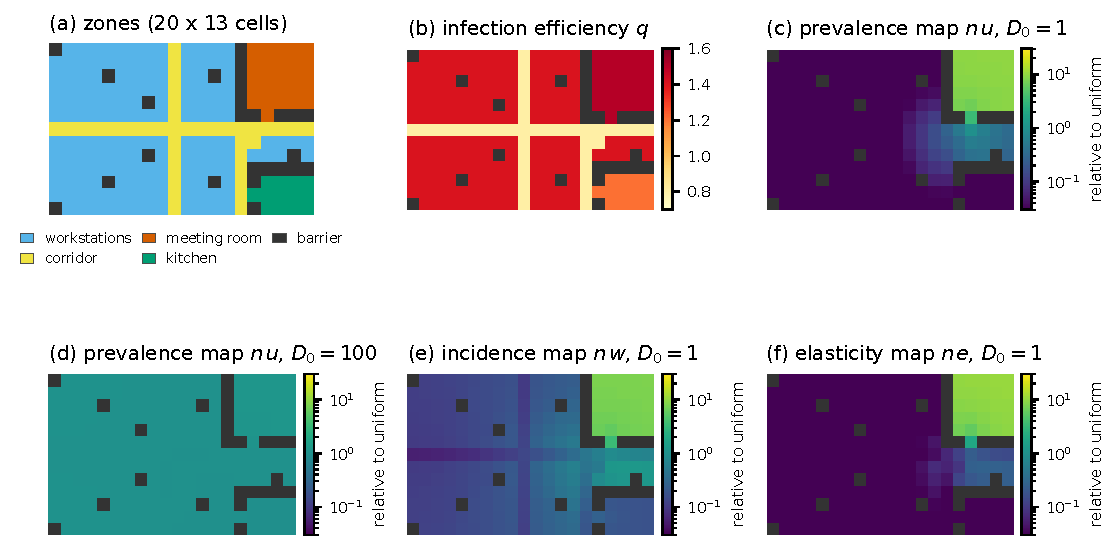
\includegraphics[width=\textwidth]{fig_hotspot_maps_en}
  \caption{Hotspot maps of the office scene in the mean-field model ($\beta=0.5\perday$,
  $\gamma=0.14\perday$, same-cell kernel; $\ncell=234$ walkable cells of the $20\times13$ lattice).
  (a) Zones. (b) Infection efficiency $q$. (c), (d) Prevalence map $\uvec$ (right Perron vector of $\Jm$) at $\Dz=1$ and $\Dz=100\cellday$.
  (e) Incidence map $\wvec$ (right Perron vector of $\ngm$) and (f) elasticity map
  $e_x=\partial\ln\Rz/\partial\ln q_x$ at $\Dz=1\cellday$. Maps are multiplied by $\ncell$, so that $1$ is the
  uniform value; the colour scale is logarithmic.}
  % src: data/plan_theory_sweeps.npz (office_u_D1, office_u_D100, office_w_D1, office_e_D1);
  %      drawn by code/plan_fig_theory.py
  \label{s4_geometry:fig:hotspots}
\end{figure}

Figure~\ref{s4_geometry:fig:hotspots} shows the maps for the office scene, in which the meeting room ($26$
cells, $11.1\,\%$ of the walkable floor of 234 cells, $q=1.5$) is joined to the rest of the floor by a single lattice edge. At
$\Dz=1\cellday$ the meeting room holds $95.9\,\%$ of $\uvec$, $79.2\,\%$ of $\wvec$ and $98.1\,\%$ of the
elasticity: $\Rz=5.107$ is in effect the reproduction number of the meeting room, whose zone bound is $5.041$.
The elasticity share of the meeting room falls to $20.8\,\%$ at $\Dz=10$ and $13.4\,\%$ at $\Dz=100\cellday$,
close to its fast-mixing limit of $12.8\,\%$.
% src: data/plan_theory_checks.json: office/zone_counts/M, office/D0=1/area_share/M;
%      data/s4_geometry_checks.json: C_office_hotspot_identities/meeting_room_boundary_edges
% src: data/plan_theory_checks.json: office/D0=1/{prevalence_share_u,incidence_share_w,elasticity_share}/M,
%      office/D0=1/R0, office/zone_bound_meeting_room/bound
% src: data/plan_theory_checks.json: office/D0=10, office/D0=100 (elasticity_share/M);
%      limit: data/s4_geometry_checks.json: C_office_hotspot_identities/meeting_room_share_limit_e_and_w
The prevalence map is an asymptotic object. It is reached after a time of order $1/\delta$, whereas the
exponential phase started by one index case among $\Npop$ people lasts about $\ln\Npop/\lamone$. At
$\Dz=1\cellday$, $1/\delta=16$ days and $\ln100/\lamone=7.6$ days: in the linearised dynamics a point seed at a
workstation far from the meeting room is still at total-variation distance $0.996$ from $\uvec$ when the total
has risen from $10^2$ to $10^4$ times the seed, so an outbreak seeded far from the hotspot does not reach the
map before saturation (Supplementary Remark~\ref{S-s4_geometry:rem:transient} in Section~\ref{S-appS_geometry:sec:hotspot}). For discrete individuals at
this mobility the mean-field maps do not describe where infections occur either
(Section~\ref{s6_scenes:sec:hotspot}).
% src: data/plan_theory_checks.json: office/D0=1/gap, office/transient_linear/D0=1|far_workstation/tv_to_u;
% src: data/s4_geometry_checks.json: D_derived/{mixing_time_1_over_gap_days,linear_phase_ln100_over_lambda1_days}

\subsection{Interventions in the mean-field model}\label{s4_geometry:sec:examples}

Supplementary Section~\ref{S-appS_geometry:sec:examples} works out interventions on the office scene. Slowing
the corridors raises $\Rz$, as Theorem~\ref{s3_r0:thm:edges} requires (corridor mobility $\times0.1$:
$5.107\to5.222$). Walls closing between $10\pct$ of the workstation--workstation edges and as many as
connectivity allows raise $\Rz$ by $0.009\pct$ to $0.080\pct$ at $\Dz=1$, and none of $80$ random draws lies
below the baseline at any of three mobilities. Turning $39$ workstation cells into barrier cells removes floor
with $q$ above the mean: the well-mixed value falls by $1.5\pct$, and $\Rz$ changes by $+0.065\pct$ at $\Dz=1$,
where it is pinned by the meeting room, and by $-1.07\pct$ and $-1.49\pct$ at $\Dz=10$ and $100$. Halving $q$ in
a targeted set of cells chosen by the elasticity map, recomputed as cells are treated, lowers $\Rz$ more than
random placement at $\Dz=1$ (by $0.35$ to $0.48$ between $5\pct$ and $75\pct$ treated area), but makes little
difference at $\Dz=100$, where targeting reduces to treating the cells with the largest $q$. Uniform measures
scale $\Rz$ exactly: multiplying $\beta$ by $s_\beta$ and every $q_x$ by $s_q$ multiplies $\Rz$ by $s_\beta s_q$.
% src: data/plan_theory_checks.json: office/corridor_multiplier_symmetric
% src: data/s4_geometry_barriers_leak.json: A_partitions/walls/*/D0=*/{change_pct,n_below_baseline}, A_partitions/barrier_cells_39_workstations
%      (wellmixed_change_pct -1.54; D0=1: +0.065; D0=10: -1.07; D0=100: -1.49)
% src: data/s4_geometry_checks.json: D_derived/targeted_ventilation/D0=1/*/gain_recomputed_vs_random (0.359, 0.352, 0.449, 0.409, 0.453, 0.482)

All of this belongs to the low-mobility regime. In the mean-field model the closed office is well mixed for
$\Dz\gtrsim100\cellday$: $\Rz=\beta\qmean/\gamma$ up to the correction of Proposition~\ref{s3_r0:prop:expansions},
the maps of Theorem~\ref{s4_geometry:thm:hotspots} reduce to $\stat$ and $\Qm\stat/\qmean$, and the floor plan
enters only through the area-weighted mean of $q$. What survives at realistic mobility is the absence of a
size effect in a closed room, the proportional scaling in $\beta$ and $q$, and the leak in its dwell-time form
\eqref{s4_geometry:eq:dwell}. A size dependence does exist for discrete individuals, for a different reason;
it is the subject of Section~\ref{s5_pair:sec}.

% m5_pair.tex -- Main text, Section 5: discrete individuals, pair-level theory.
% Paths in "% src:" comments are relative to the repository root.
% Numbers not stored verbatim in the research directories are recomputed by code/s5_pair_checks.py
% -> data/s5_pair_checks.json (table bodies: data/s5_pair_tables.tex).  Proofs:
% Supplementary Section S4.
\section{Discrete individuals: a pair-level theory}\label{s5_pair:sec}

The next-generation matrix of Section~\ref{s3_r0:sec} counts infectious \emph{contacts}: its column sum
$\noff(x)$, eq.~\eqref{s3_r0:eq:offspring}, is the expected time-integrated transmission rate of a case born in
cell $x$. In the mean-field model every contact meets a fresh susceptible. In the individual-based model of
Section~\ref{s2_model:sec:ibm} this is not so: each person can be infected only once, and an infective who moves
slowly keeps meeting the same few neighbours, so that later contacts with a person already infected are
wasted. This local saturation of contacts is classical. It is the reason why epidemics with household
structure need reproduction numbers defined for groups and not for individuals \citep{ball1997epidemics},
why pair approximations on lattices and networks predict slower invasion than mass action
\citep{keeling1999effects}, and more generally why discrete spatial models differ from their mean-field
equations \citep{durrett1994importance}. At the default parameters (0.43 people per cell, $\Dz=1\cellday$) the
effect is a factor of two: a lone index case in the office scene infects on average $2.27$ people, against
$\Rz=5.11$.
% src: data/bsc_sim/02_mobility.json (D0_1.0: R1_pair_uniform_index 2.266, R0_ngm 5.107)

Treating infection as a reaction between two random walkers is not new. \citet{kenkre2014theory} and
\citet{sugaya2018analysis} computed the infection probability of a pair of walkers with and without
confinement, and the approach is developed in the monograph of \citet{kenkre2021theory}. Closest to what
follows, \citet{giuggioli2022spatio} map transmission at co-location onto a partially absorbing site of the
two-walker lattice walk in discrete time. For one infected walker among $W$ susceptible walkers with
uniformly random initial positions and a geometric infectious period they obtain the mean number of
secondary infections as $W$ times the position-averaged generating function of the transmission
probability (their Section~6), call it the basic reproduction number, and check it against simulations in a
square domain with reflecting walls. The number $\Ronebar$ defined below is the continuous-time counterpart
of that quantity. The solution technique for one partially absorbing site goes back to
\citet{szabo1984localized}; lattice formulations with several reactive defects are given by
\citet{giuggioli2020exact} and \citet{giuggioli2022spatio}, and the analogous formalism for inert
heterogeneities by \citet{sarvaharman2023particle}. What is added here is listed in Section~\ref{s1_intro:sec}.
% src: data/refs_search.json (searches; Crossref abstracts of giuggioli2022spatio and sarvaharman2023particle: reactive against inert heterogeneities)

\subsection{The pair problem}\label{s5_pair:sec:pair}

Throughout this section movement follows the symmetric rule \eqref{s2_model:eq:hop}, so that $\gen$ is
symmetric and $\pi_x=1/\ncell$, and the $\Npop$ people start independently from the uniform distribution.
One of them, the index case, becomes infectious at time $0$ in cell $x$ and stays infectious for a time
$\tau$ that is exponential with rate $\gamma$ and independent of the movement. Consider one other person,
who is in cell $y$ at time $0$. The pair $Z_t=(X_t,Y_t)$ is a Markov chain on $\cells\times\cells$ with
generator $\mathcal{M}=\gen\otimes\Id+\Id\otimes\gen$ (column index = source state). While the pair is in
state $(x',y')$ the index infects the other person at the rate $h(x',y')=\beta q_{x'}P_{x'y'}/\rhobar$ of
eq.~\eqref{s2_model:eq:pairhazard}, where $\rhobar=(\Npop-1)/\ncell$.

\begin{proposition}[Pair infection probability]\label{s5_pair:prop:pair}
  Let $p(x,y)$ be the probability that the index case infects the given other person before recovering, when
  no one else transmits.  With $\mathcal{M}=\gen\otimes\Id+\Id\otimes\gen$ and $\mathbf{H}=\diag\,h$ on
  $\cells\times\cells$,
  \begin{equation}\label{s5_pair:eq:pair}
     \one-p=\gamma\bigl(\gamma\Id+\mathbf{H}-\mathcal{M}^{\T}\bigr)^{-1}\one .
  \end{equation}
\end{proposition}

Equation \eqref{s5_pair:eq:pair} is the Feynman--Kac formula
$1-p(z)=\Exp_z\exp\bigl(-\int_0^{\tau}h(Z_t)\,\dd t\bigr)$ for the pair chain killed at rate $\gamma+h$:
infection is a partially absorbing defect of the two-walker process. Since $\gen$ is symmetric, the matrix in
\eqref{s5_pair:eq:pair} is symmetric positive definite, and the system is solved by conjugate gradients on the
$\ncell^2$ pair states ($54{,}756$ for the office scene).

\begin{definition}[Pair-level reproduction numbers]\label{s5_pair:def:R1}
  $\Rone(x)=(\Npop-1)\,\ncell^{-1}\sum_{y}p(x,y)$ is the expected number of secondary cases of a lone index case
  born at $x$ when the other $\Npop-1$ people are susceptible, independent and uniformly distributed and only
  the index transmits; $\Ronebar=\ncell^{-1}\sum_x\Rone(x)$.  The pair-level next-generation matrix
  $\ngmone$ has entries $(K_1)_{zx}$ = expected number of people infected by that index case \emph{while they
  are located in cell $z$}; its column sums are $\Rone(x)$.
\end{definition}

$\Rone(x)$ is exact for the individual-based model: the $\Npop-1$ pairs formed by the index and each other
person are identically distributed, and although they are dependent (they share the index's path and
infectious period) expectations add. When later cases also transmit, the index infects at most as many
people, since some are infected by others first. $\ngmone$ is obtained from $\ncell$ further linear solves;
for the scenes of this article all of them take a few seconds.
% src: data/s5_pair_checks.json (saturation/*/seconds: 0.9-4.7 s for K, K1 and p)

\begin{proposition}[Saturation]\label{s5_pair:prop:saturation}
  For every scene, every row-stochastic contact kernel and every $\Npop\ge2$,
  $0\le(K_1)_{zx}\le K_{zx}$ for all $z,x$, with strict inequality wherever $K_{zx}>0$.  Consequently
  $\Rone(x)<\noff(x)$ for every $x$, $\Ronebar<\beta\langle q\rangle/\gamma$ and $\srad(\ngmone)\le\Rz$.
\end{proposition}

The mean-field matrix thus counts exposure, and the pair-level matrix discounts the exposure of people who
are already infected. For the same-cell kernel Theorem~\ref{s3_r0:thm:bounds} gives
$\Ronebar<\beta\langle q\rangle/\gamma\le\Rz$: a uniformly placed lone index case infects fewer people than
even the well-mixed lower bound of $\Rz$.

\subsection{Homogeneous periodic rooms: a closed form}\label{s5_pair:sec:closed}

\begin{proposition}[Homogeneous periodic room]\label{s5_pair:prop:torus}
  On an $L_1\times L_2$ periodic lattice with hop rate $D$ to each of the four neighbours, uniform $q$ and the
  same-cell kernel, let $h_0=\beta q/\rhobar$.  Then $p(x,y)=h_0\,g(y-x)/(1+h_0\,\gz)$, where
  $g(r)=\int_0^\infty\e^{-\gamma t}\,\Prob(\text{relative walk at }0\text{ at time }t\mid\text{start at }r)\,\dd t$
  and $\gz=g(0)$, and
  \begin{equation}\label{s5_pair:eq:R1}
     \Rone=\frac{\beta q/\gamma}{1+(\beta q/\rhobar)\,\gz},\qquad
     \gz=\frac1{\ncell}\sum_{k}\frac{1}{\gamma+2\mu_k},\qquad
     \mu_k=2D\,(2-\cos k_1-\cos k_2),
  \end{equation}
  where $k=(k_1,k_2)$ runs over $\tfrac{2\pi}{L_1}\{0,\dots,L_1-1\}\times\tfrac{2\pi}{L_2}\{0,\dots,L_2-1\}$.
  $\Rone$ is increasing in $D$ and in $\rhobar$.  Limits: $D\to\infty$ at fixed $\ncell$:
  $\Rone\to(\beta q/\gamma)/\bigl(1+\beta q/(\gamma(\Npop-1))\bigr)$; $D\to0$: $\Rone\to\rhobar h_0/(h_0+\gamma)$.
\end{proposition}

Formula \eqref{s5_pair:eq:R1} has the structure of a renewal argument. If infectious contacts with the given
person continued after infection, their expected number would be $h_0\,g(r)$, the mean-field exposure. Given
that there is at least one contact, the pair is co-located at that moment and the expected number of contacts
is $1+h_0\gz$. The ratio of the two is the probability of at least one contact. The two limits are the
Markovian epidemic in a well-mixed population of $\Npop$ people, where each pair interacts at rate
$\beta q/(\Npop-1)$, and a frozen room, where the index infects only the $\rhobar$ people who share its cell
on average, each with probability $h_0/(h_0+\gamma)$. A direct solve of \eqref{s5_pair:eq:pair} on four
periodic lattices reproduces \eqref{s5_pair:eq:R1} to 13 digits.
% src: data/s5_pair_checks.json (torus: abs_err <= 7e-14); data/plan_theory_checks.json
%      (checks/torus_L5_N11: 2.316775601727); code/bsc_sim/verify/v04_finite.json (torus_L6_D1.0, torus_L8_D0.51)

\begin{corollary}[Infinite floor]\label{s5_pair:cor:infinite}
  For $L_1,L_2\to\infty$ at fixed $\rhobar$,
  $\gz=\dfrac{2}{\pi}\,\dfrac{\mathcal{K}(k_*)}{\gamma+8D}$ with modulus $k_*=\dfrac{8D}{\gamma+8D}$, where
  $\mathcal{K}$ is the complete elliptic integral of the first kind.  In particular $\Rone<\beta q/\gamma$ for
  every finite $D$: the correction does not vanish for large rooms.
\end{corollary}

For $8D\gg\gamma$ the logarithmic singularity of $\mathcal{K}$ gives $\gz\approx\ln(64D/\gamma)/(8\pi D)$: the
correction decays with mobility only as $\ln D/D$, which reflects the recurrence of the planar walk.

\begin{observation}[Reflecting walls]\label{s5_pair:obs:reflecting}
  For a rectangular room with reflecting walls, formula \eqref{s5_pair:eq:R1} with
  $\mu_k=2D(2-\cos(k_1\pi/L_1)-\cos(k_2\pi/L_2))$, $k_i=0,\dots,L_i-1$ (cell-averaged $\gz$) reproduces
  $\Ronebar$ from the exact pair solve \eqref{s5_pair:eq:pair} to within $0.9\,\%$ for $L=4,\dots,28$ and
  $D=0.51,1,10$ (largest deviation at $D=0.51$, $L=7$).
\end{observation}
% src: data/bsc_sim/02_finite_size.json (pair_closed_form, pair_exact);
%      data/s5_pair_checks.json (finite_size: max 0.90 % at D0.51_L7; by D: 0.90 %, 0.46 %, 0.02 %)

\subsection{The form of a finite-size effect}\label{s5_pair:sec:finite}

For the mean-field model a closed room has no size effect (Theorem~\ref{s4_geometry:thm:closed}). Discrete
people do show a size effect, and \eqref{s5_pair:eq:R1} is its form. Fig.~\ref{s5_pair:fig:finite} (numbers in
Supplementary Table~\ref{S-s5_pair:tab:finite}) compares the mean-field number, the closed form, the exact pair
solve and simulation in homogeneous $L\times L$ rooms with $0.381$ other people per cell (99 people on the 260
cells of a $20\times13$ lattice without barriers; the office scene, with 234 walkable cells, has $0.423$).
% src: data/bsc_sim/02_finite_size.json (rho_bar = 99/260); data/s2_model_scenes.json -> scenes.office.rho_bar (0.4231)

\begin{figure}[tbp]
\centering
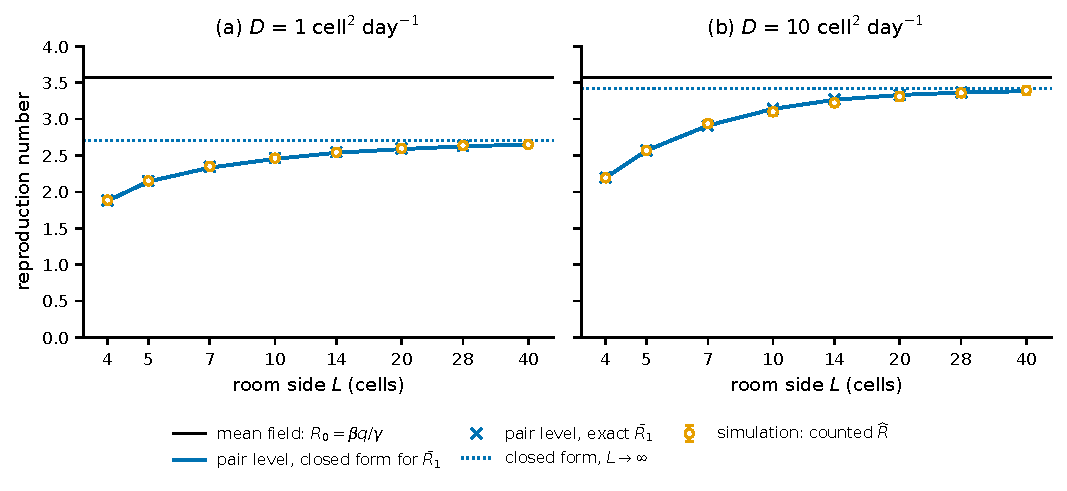
\includegraphics[width=\textwidth]{fig5_1_finite_size_en}
\caption{Finite-size effect for discrete people. Homogeneous $L\times L$ rooms with reflecting walls, $q=1$,
same-cell kernel, $\rhobar\approx0.381$ others per cell ($\Npop=7$ at $L=4$ to $610$ at $L=40$), mobility
(a) $D=1$ and (b) $D=10\cellday$. Black line: mean-field $\Rz=\beta q/\gamma=3.571$. Blue line: closed form
\eqref{s5_pair:eq:R1} with the reflecting-wall spectrum; crosses: exact pair solve \eqref{s5_pair:eq:pair}
($L\le28$); dotted line: infinite lattice (Corollary~\ref{s5_pair:cor:infinite}). Circles: counted secondary
cases $\Rhat$ of a uniformly placed index case when only the index transmits, 20{,}000 runs per point, bars are
95\pct{} confidence intervals.}
\label{s5_pair:fig:finite}
% src: data/bsc_sim/02_finite_size.json; figure script code/fig_finite_size.py
\end{figure}

At $D=1$ a lone index case infects on average $1.88$ people in a $4\times4$ room with 7 people, $2.60$ in a
$20\times20$ room with 153 people and $2.71$ on an infinite floor at the same occupancy, against $3.57$ in the
mean-field model at every size. The correction is a lattice Green's function. It decreases with mobility: at
$L=10$ the counted number rises from $2.46$ at $D=1$ to $3.10$ at $D=10$. And it does not vanish as
$L\to\infty$: the infinite-floor value is $76\,\%$ of $\beta q/\gamma$ at $D=1$ and $96\,\%$ at $D=10$. The cause
is the repeated meeting of the same people, in a small room because there are few of them and on a large floor
because a slow planar walker returns to its neighbours; nothing leaks through the walls. The closed form lies
inside the 95\,\% interval of the counted value in 23 of the 24 rooms scanned, and the exact solve in 19 of
the 21 rooms for which it was computed; the second simulator agrees with the exact solve within $1.7$ standard
errors in the seven rooms re-run, including the two exceptions.
% src: data/bsc_sim/02_finite_size.json; data/s5_pair_checks.json
%      (finite_size/ratio_to_meanfield: D1.0_Linf 0.759, D10.0_Linf 0.958; closed_outside_sim_ci, exact_outside_sim_ci;
%      finite_size_check: z between -1.35 and 1.65); code/bsc_sim/verify/v04_finite.json

\subsection{Mobility: opposite trends at the two levels}\label{s5_pair:sec:mobility}

\begin{figure}[tbp]
\centering
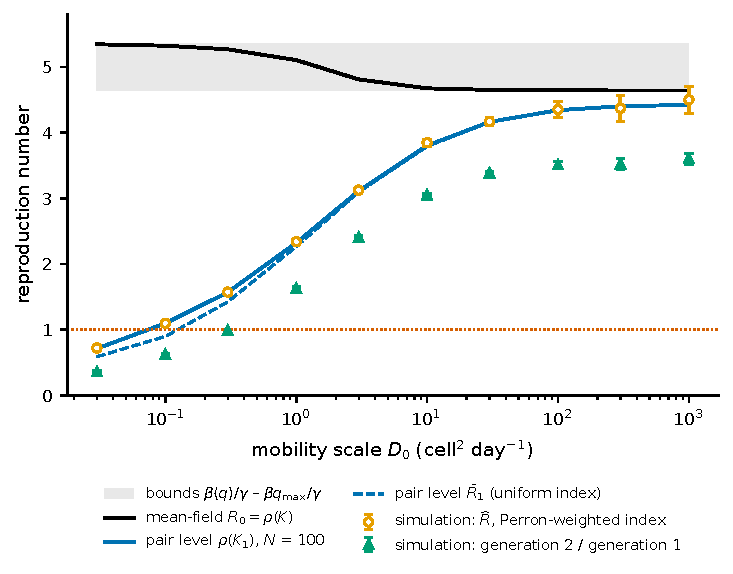
\includegraphics[width=0.72\textwidth]{fig5_5_R_vs_mobility_en}
\caption{Reproduction numbers of the office scene against the mobility scale $\Dz$ ($\Npop=100$, same-cell
kernel, $\beta=0.5\perday$, $\gamma=0.14\perday$). Black line: mean-field $\Rz=\srad(\ngm)$; grey band: its
bounds $\beta\langle q\rangle/\gamma=4.643$ and $\beta\qmax/\gamma=5.357$. Solid blue line: the spectral
radius $\srad(\ngmone)$ of the pair-level next-generation matrix; dashed blue line: the average $\Ronebar$
over a uniformly placed index case, which is lower at small $\Dz$. Circles: counted secondary cases $\Rhat$ of an
index case born according to the Perron vector of $\ngmone$ when only the index transmits. Triangles: number
of second-generation cases divided by the number of first-generation cases when the index and its direct
cases transmit. Bars are 95\pct{} confidence intervals; numbers of runs and values in
Supplementary Table~\ref{S-s5_pair:tab:mobility}. The dotted line marks the value one.}
\label{s5_pair:fig:mobility}
% src: data/bsc_sim/02_mobility.json; figure script code/bsc_sim/experiments/21_figures_more.py
\end{figure}

The mean-field $\Rz$ of the office scene decreases with mobility (Theorem~\ref{s3_r0:thm:mobility}), from
$5.35$ at $\Dz=0.03$ to $4.64$ at $\Dz=1000$; the pair-level numbers increase, $\Ronebar$ from $0.59$ to $4.42$:
a faster index case meets more distinct people (Fig.~\ref{s5_pair:fig:mobility}). At $\Dz=1$, $\Ronebar=2.27$
is $44\,\%$ of $\Rz=5.11$; at $\Dz=10$ it is $81\,\%$ and at $\Dz=100$ it is $93\,\%$. At $\Dz=1000$,
$\Ronebar=4.425$ is close to $(\beta\langle q\rangle/\gamma)/\bigl(1+\beta\langle q\rangle/(\gamma(\Npop-1))\bigr)=4.435$,
the value for a well-mixed population of 100 people (compare the limit $D\to\infty$ in
Proposition~\ref{s5_pair:prop:torus}). Counted secondary cases agree: samples of 400{,}000, 400{,}000 and
100{,}000 runs give $2.265\pm0.004$, $3.793\pm0.006$ and $4.340\pm0.015$ at $\Dz=1$, $10$ and $100$, against
$\Ronebar=2.266$, $3.793$ and $4.341$.
% src: data/bsc_sim/02_mobility.json; data/s5_pair_checks.json (mobility: R1bar_over_R0
%      0.444, 0.811, 0.934; office_wellmixed_finite_population 4.4349)
% src: data/s5_pair_large_sample.json (office|D0=1: mean 2.2648, se 0.0039; office|D0=10: 3.7930, 0.0064; office|D0=100: 4.3399, 0.0145)
On the infinite homogeneous lattice at $\rhobar=0.381$ and $\beta q=0.5\perday$ the ratio $\Rone/\Rz$ is $0.5$
at $D=0.24$, $0.9$ at $D=3.5$ and $0.99$ at $D=52\cellday$ (Supplementary Fig.~\ref{S-s5_pair:fig:validity}). The
mean-field number is therefore adequate when many people share a contact neighbourhood or when people move far
enough during an infectious period to meet new ones; the scenes at $\Dz=1$ satisfy neither condition. At
$\Dz\approx2.4\times10^3\cellday$ (Section~\ref{s2_model:sec:regime}) the ratio on the infinite lattice is
$0.9997$, and what remains in a finite room is the well-mixed finite-population factor.
% src: data/s5_pair_checks.json (infinite: D_for_ratio_*; D=2400 ratio 0.99970)

\subsection{Later generations: not a threshold}\label{s5_pair:sec:threshold}

The pair level is exact for the first generation and stops there. A secondary case is not a lone index case:
it starts in or next to the cell of its infector, who cannot be infected again, and near the other cases its
infector has caused, so part of its neighbourhood is already used up. In the office at $\Dz=1$ the second
generation is $1.63$ ($1.61$--$1.65$) times the first, against $\srad(\ngmone)=2.32$. The ratio of these two
numbers is $0.50$ at $\Dz=0.03$, $0.70$ at $\Dz=1$ and $0.80$--$0.81$ for $\Dz\ge10$; the last value is that
of a well-mixed population of 100, in which the index and its direct cases compete for the same susceptibles
($0.81$ in $200{,}000$ runs of the well-mixed model with the same design).
% src: data/bsc_sim/02_mobility.json (sim_gen2_over_gen1, R1_pair_ngm); data/s5_pair_checks.json
%      (mobility: gen_ratio_over_rhoK1; wellmixed_generation_ratio: 3.589 / 4.435 = 0.809)

\begin{remark}[$\Rone$ and $\srad(\ngmone)$ are not threshold quantities]\label{s5_pair:rem:threshold}
Neither $\Ronebar>1$ nor $\srad(\ngmone)>1$ implies that large outbreaks are possible. In the metro
carriage with the same-cell kernel at $\Dz=1$ ($310$ people on $270$ cells; in the median cell a passenger
waits 48 days between hops) $\srad(\ngmone)=2.24$ and $\Ronebar=1.51$, and the counted number of secondary cases of a lone index
case is $1.52$ ($1.49$--$1.54$; 20{,}000 runs). Yet the second generation is $0.61$ times the first, and no
outbreak reached $10\pct$ of the passengers in 2{,}000 runs of one simulator and 3{,}000 of another (mean
attack rate $1.1\pct$): the index infects the people in its own cell, and they have no one left to infect. The
mean-field value for the same case is $\Rz=9.84$. An intervention must therefore not be judged by
`$\Rone<1$', and $\srad(\ngmone)$ should not be read as a basic reproduction number of the discrete
system. That a threshold exists for infection among lattice random walkers is known: rigorously for
independent walkers on $\mathbb{Z}^d$ with recovery and reinfection \citep{kesten2006phase}, and from
simulations of the diffusive epidemic process, including its variant with permanent immunity
\citep{maia2007diffusive,carvalho2025generalized}. Those results concern infinite or large homogeneous
lattices and do not give a computable threshold for the small heterogeneous rooms considered here. No
quantity in this article predicts the threshold or the final size of the individual-based model at low
mobility; these are obtained by simulation in Section~\ref{s6_scenes:sec}.
\end{remark}
% src: data/bsc_sim/03_scenes.json (metro|D0=1|samecell: R1_pair_ngm 2.2437, R1_pair_uniform_index 1.5138,
%      R0_ngm 9.836, n_major 0 of 2000, attack_all_mean 0.0112, gen2_over_gen1 0.608);
%      code/bsc_sim/verify/v05_scenes.json (metro|1.0|same: 0 of 3000, gen2_over_gen1 0.609);
%      data/bsc_sim/01_validation.json (D_pair_theory, metro same cell: 1.517, 1.495-1.539);
%      data/s5_pair_checks.json (saturation/metro: rho_K1 2.2437, R1bar 1.5138, median_cell_time_between_hops_days 48.5)

In summary, three numbers describe the first steps of an outbreak among discrete people at low mobility, and
they must be kept apart: the mean-field $\Rz$, which counts exposure and whose matrix bounds the pair-level
one from above (Proposition~\ref{s5_pair:prop:saturation}); the pair-level $\Rone(x)$, which is the exact
expected number of people a lone index case infects; and the growth from one generation to the next, which
is lower again and for which we have no formula.

% m6_simulation.tex -- Main text, Section 6: exact stochastic simulation of four indoor scenes and of interventions.
% Paths in "% src:" comments are relative to the repository root.
% Table bodies between "% BEGIN AUTO" and "% END AUTO" are written by code/s6_scenes_tables.py
% (-> data/s6_scenes_tables.tex) and pasted by code/s6_scenes_paste_tables.py; every
% derived number quoted in the prose is stored in data/s6_scenes_numbers.json (key given in the comment).
% Details, further tables and figures: Supplementary Section S5.
\section{Exact stochastic simulation of four indoor scenes}\label{s6_scenes:sec}

Sections~\ref{s3_r0:sec}--\ref{s5_pair:sec} gave two reproduction numbers that are computed without simulation:
the mean-field $\Rz$ and the pair-level $\Ronebar$. This section reports what the individual-based model of
Section~\ref{s2_model:sec:ibm} does in the four scenes of Table~\ref{s2_model:tab:scenes}, how far each number
describes it, and what the model says about interventions. All results are given for $\Dz=1$, $10$ and
$100\cellday$, which all lie far below walking mobility (Section~\ref{s2_model:sec:regime}); the departures from
mean-field theory reported below are large at $\Dz=1$ and small at $\Dz=100$.

\subsection{Simulator and protocol}\label{s6_scenes:sec:protocol}

The individual-based model is simulated exactly, event by event (Supplementary
Fig.~\ref{S-appA_numerics:fig:algorithm}); secondary cases are counted on the recorded infection tree. Each
replicate has its own stream of the xoshiro256** generator \citep{blackman2021scrambled}. The simulator agrees in
distribution with a separately written pure-Python implementation, with the exact final-size law of the
one-cell model, with the next-generation matrix through an exposure identity, and with the mean-field equations
at high occupancy and mobility (Supplementary Table~\ref{S-appA_numerics:tab:simulator}). The scene results at
$\Dz=1$ and most of those at $\Dz=10$ were in addition re-run with the second simulator; the two agree within
Monte Carlo error, the two largest differences being $1.6$ and $2.1$ standard errors (Supplementary
Section~\ref{S-appS_sim:sec:scenes}).
% src: code/bsc_sim/verify/v05_scenes.json (p_major, n); data/s6_scenes_numbers.json: check_scenes.*.z_first_minus_check (1.56, 2.11)

People start from the stationary (uniform) distribution and one of them, hence at a uniformly distributed
cell, is infectious at time $0$. For each scene, mobility and contact kernel, 2{,}000 epidemics are run until no
infective is left. The \emph{attack rate} is the fraction of the $\Npop$ people ever infected, the index case
included. An outbreak is called \emph{major} if its attack rate is at least $10\,\%$, and $P_{\mathrm{maj}}$ is
the fraction of major outbreaks, with a Wilson $95\,\%$ interval; the threshold is a convention whose influence
is quantified in Supplementary Section~\ref{S-s6_scenes:sec:pmajor}. The counted number of secondary cases
$\Rhat$ is the mean over 2{,}000 further runs in which only the index case transmits. The mean-field
counterparts are $\Rz$, the solution of \eqref{s2_model:eq:meanfield}, and the outbreak probability
$P_{\mathrm{br}}$ of the branching process in which a case walks with generator $\gen$, recovers at rate
$\gamma$ and, while in cell $x$, produces new cases at rate $\beta q_x$ placed in cell $y$ with probability
$P_{xy}$; the extinction probabilities $s_x$ of its lines of descent are the minimal non-negative solution
\citep{andersson2000stochastic} of
\begin{equation}\label{s6_scenes:eq:branching}
  \gamma\,(1-s_x)+\beta q_x\,s_x\Bigl(\sum_{y}P_{xy}s_y-1\Bigr)+\sum_{y}\hop{x}{y}\,(s_y-s_x)=0 ,
  \qquad P_{\mathrm{br}}=1-\frac1{\ncell}\sum_{x\in\cells}s_x
\end{equation}
% src: code/bsc_sim/experiments/03_scenes.py (n_rep = 2000, T_MAX = 400 d); code/bsc_sim/src/bsc_sim/theory.py (extinction_probability, meanfield_ode)

\subsection{Outcomes in the four scenes}\label{s6_scenes:sec:outcomes}

\begin{table}[tbp]
\centering
\caption{The four scenes in exact simulation and in mean-field theory, for mobility scale $\Dz$ (cell$^2$ per
day), $\beta=0.5\perday$, $\gamma=0.14\perday$, frequency-dependent incidence; 2{,}000 epidemics per row, one
uniformly placed index case, closed room. $\Rz$: mean-field basic reproduction number. $\Ronebar$: pair-level
expected number of secondary cases of a uniformly placed index case (Definition~\ref{s5_pair:def:R1}).
$\Rhat\pm$SE: counted mean number of secondary cases, index case alone transmitting (2{,}000 further runs).
$P_{\mathrm{maj}}$: fraction of runs with attack rate at least $10\,\%$ (Wilson interval). $P_{\mathrm{br}}$:
mean-field branching value \eqref{s6_scenes:eq:branching}. Attack rate: mean over major outbreaks and over all
runs. Peak: mean over major outbreaks of the maximal prevalence (0.5-day grid) and of its day. ODE: attack rate
(\%) / peak prevalence (\%) / peak day of the mean-field equations started from one infective spread uniformly,
and peak prevalence (\%) / peak day for one infective in a single cell (mean over seed cells; 1\,m kernel
only). A dash means that there was no major outbreak.}
\label{s6_scenes:tab:scenes}
% src: data/bsc_sim/03_scenes.json (all columns but the last); data/s6_scenes_ode_pointseed.json (last column)
\footnotesize
\setlength{\tabcolsep}{2.7pt}
\begin{tabular}{@{}rccccccccccc@{}}
\toprule
 & & & & & & \multicolumn{2}{c}{attack rate (\%)} & \multicolumn{2}{c}{peak} & \multicolumn{2}{c}{mean-field ODE}\\
\cmidrule(lr){7-8}\cmidrule(lr){9-10}\cmidrule(l){11-12}
$\Dz$ & $\Rz$ & $\Ronebar$ & $\Rhat\pm{}$SE & $P_{\mathrm{maj}}$ (95\,\% CI) & $P_{\mathrm{br}}$ & major & all &
\% & day & uniform seed & point seed\\
\midrule
% BEGIN AUTO s6_scenes:tab:scenes
\multicolumn{12}{@{}l}{\emph{Office}, $\Npop=100$, $\ncell=234$, 1\,m kernel (identical to the same-cell kernel); $\beta\langle q\rangle/\gamma=4.64$, $\beta\qmax/\gamma=5.36$}\\
1 & 5.11 & 2.27 & 2.26\,$\pm$\,0.06 & 0.496 (0.474--0.518) & 0.781 & 44.3 & 23.2 & 12.7 & 23.2 & 98.9 / 45.1 / 11.5 & 32.8 / 20.4\\
10 & 4.68 & 3.79 & 3.90\,$\pm$\,0.09 & 0.762 (0.743--0.781) & 0.783 & 96.3 & 73.8 & 39.0 & 16.5 & 99.0 / 45.7 / 11.5 & 44.1 / 12.8\\
100 & 4.65 & 4.34 & 4.11\,$\pm$\,0.10 & 0.770 (0.751--0.788) & 0.784 & 98.8 & 76.4 & 48.4 & 12.6 & 99.0 / 45.9 / 11.5 & 45.9 / 11.6\\
\addlinespace
\multicolumn{12}{@{}l}{\emph{Supermarket}, $\Npop=150$, $\ncell=278$, 1\,m kernel (identical to the same-cell kernel); $\beta\langle q\rangle/\gamma=3.26$, $\beta\qmax/\gamma=7.14$}\\
1 & 4.39 & 1.99 & 1.97\,$\pm$\,0.05 & 0.436 (0.414--0.458) & 0.667 & 42.0 & 19.4 & 10.1 & 31.5 & 93.6 / 28.9 / 17.0 & 23.7 / 25.7\\
10 & 3.39 & 2.86 & 2.86\,$\pm$\,0.07 & 0.648 (0.627--0.669) & 0.685 & 92.1 & 60.0 & 30.6 & 22.6 & 95.4 / 33.4 / 17.5 & 33.1 / 18.0\\
100 & 3.28 & 3.15 & 3.04\,$\pm$\,0.08 & 0.686 (0.665--0.706) & 0.692 & 95.3 & 65.7 & 36.1 & 19.3 & 95.7 / 33.7 / 18.5 & 33.7 / 18.3\\
\addlinespace
\multicolumn{12}{@{}l}{\emph{Classroom}, $\Npop=80$, $\ncell=148$, 1\,m kernel (4.6 cells on average); $\beta\langle q\rangle/\gamma=4.71$, $\beta\qmax/\gamma=7.14$}\\
1 & 5.87 & 2.58 & 2.62\,$\pm$\,0.06 & 0.614 (0.592--0.635) & 0.767 & 39.2 & 25.2 & 14.1 & 16.3 & 98.4 / 42.6 / 11.0 & 31.7 / 18.1\\
10 & 4.93 & 3.72 & 3.72\,$\pm$\,0.09 & 0.750 (0.731--0.768) & 0.777 & 94.0 & 70.9 & 35.0 & 17.3 & 98.8 / 45.0 / 10.5 & 41.3 / 12.8\\
100 & 4.73 & 4.32 & 4.30\,$\pm$\,0.10 & 0.779 (0.760--0.797) & 0.785 & 98.6 & 77.2 & 48.8 & 12.2 & 99.1 / 46.5 / 11.0 & 46.5 / 11.0\\
\addlinespace
\multicolumn{12}{@{}l}{\emph{Classroom}, $\Npop=80$, $\ncell=148$, same-cell kernel; $\beta\langle q\rangle/\gamma=4.71$, $\beta\qmax/\gamma=7.14$}\\
1 & 6.18 & 1.56 & 1.53\,$\pm$\,0.04 & 0.276 (0.256--0.295) & 0.766 & 19.7 & 7.6 & 8.5 & 15.2 & 98.0 / 40.0 / 11.0 & \\
10 & 4.96 & 3.20 & 3.15\,$\pm$\,0.07 & 0.695 (0.674--0.715) & 0.777 & 89.1 & 62.5 & 29.7 & 20.7 & 98.8 / 44.5 / 10.5 & \\
100 & 4.73 & 4.23 & 4.39\,$\pm$\,0.10 & 0.771 (0.753--0.789) & 0.785 & 98.6 & 76.4 & 48.2 & 12.3 & 99.1 / 46.5 / 11.0 & \\
\addlinespace
\multicolumn{12}{@{}l}{\emph{Metro carriage}, $\Npop=310$, $\ncell=270$, 1\,m kernel (11.1 cells on average); $\beta\langle q\rangle/\gamma=9.06$, $\beta\qmax/\gamma=10.00$}\\
1 & 9.24 & 5.58 & 5.59\,$\pm$\,0.10 & 0.879 (0.864--0.893) & 0.888 & 93.7 & 82.4 & 24.9 & 21.9 & 100.0 / 64.1 / 7.0 & 35.0 / 16.3\\
10 & 9.16 & 6.32 & 6.44\,$\pm$\,0.13 & 0.878 (0.863--0.892) & 0.888 & 98.4 & 86.5 & 27.5 & 21.0 & 100.0 / 64.3 / 7.0 & 36.3 / 15.7\\
100 & 9.08 & 7.54 & 7.58\,$\pm$\,0.16 & 0.891 (0.877--0.904) & 0.889 & 99.9 & 89.0 & 35.3 & 16.5 & 100.0 / 64.6 / 7.0 & 42.2 / 13.8\\
\addlinespace
\multicolumn{12}{@{}l}{\emph{Metro carriage}, $\Npop=310$, $\ncell=270$, same-cell kernel; $\beta\langle q\rangle/\gamma=9.06$, $\beta\qmax/\gamma=10.00$}\\
1 & 9.84 & 1.51 & 1.56\,$\pm$\,0.04 & 0.000 (0.000--0.002) & 0.888 & -- & 1.1 & -- & -- & 100.0 / 61.4 / 7.0 & \\
10 & 9.31 & 3.00 & 3.05\,$\pm$\,0.07 & 0.349 (0.329--0.371) & 0.888 & 17.3 & 7.7 & 5.0 & 23.4 & 100.0 / 62.9 / 7.0 & \\
100 & 9.09 & 6.10 & 6.24\,$\pm$\,0.14 & 0.858 (0.842--0.873) & 0.889 & 98.6 & 84.7 & 24.0 & 24.4 & 100.0 / 64.4 / 7.0 & \\
% END AUTO s6_scenes:tab:scenes
\bottomrule
\end{tabular}
\end{table}

\paragraph{Secondary cases.} The pair-level $\Ronebar$ reproduces the counted $\Rhat$ in all 18 rows of
Table~\ref{s6_scenes:tab:scenes}: the largest deviation is $2.3$ standard errors (office, $\Dz=100$) and no
other row exceeds $2$. The mean-field $\Rz$ does not: at $\Dz=1$ the ratio $\Rhat/\Rz$ is $0.44$, $0.45$,
$0.45$ and $0.60$ in the office, supermarket, classroom and metro carriage, rising to $0.84$--$0.93$ at
$\Dz=100$. Later generations grow more slowly still: over the full epidemics at $\Dz=1$ the second generation
is $1.29$, $1.38$, $1.32$ and $1.84$ times as numerous as the first (second simulator: $1.39$, $1.40$, $1.29$,
$1.87$), where $\srad(\ngmone)=2.32$, $2.20$, $2.83$ and $5.72$.
% src: data/s6_scenes_numbers.json: Rhat_vs_R1bar (largest_abs_z = 2.28, n_rows_abs_z_gt_2 = 1)
% src: data/bsc_sim/03_scenes.json (R_index_alone_mean, R0_ngm); s6_scenes_numbers.json: scenes.*.Rhat_over_R0
% src: data/bsc_sim/03_scenes.json: gen2_over_gen1, R1_pair_ngm (rows D0 = 1, range1m);
%      code/bsc_sim/verify/v05_scenes.json: gen2_over_gen1 (1.388, 1.397, 1.291, 1.869)

\paragraph{Low mobility, $\Dz=1$.} The mean-field description fails for every whole-epidemic outcome in the
office, the supermarket and the classroom. In the office $P_{\mathrm{maj}}=0.496$ ($0.474$--$0.518$) against
$P_{\mathrm{br}}=0.781$; major outbreaks infect $44.3\,\%$ ($95\,\%$ interval of the mean $42.9$--$45.6\,\%$) of
the people where the mean-field equations give
$98.9\,\%$, and their prevalence peaks at $12.7\,\%$ on day $23.2$ where the mean-field equations give $45.1\,\%$
on day $11.5$ from a uniform seed and $32.8\,\%$ on day $20.4$ from a single cell. The attack-rate distributions
are not bimodal: $27\,\%$, $28\,\%$ and $43\,\%$ of all runs end with an attack rate between $10\,\%$ and
$50\,\%$, against at most $0.6\,\%$ at $\Dz=10$. Spread is local and slow, and outbreaks stall at every size.
The metro carriage is closer to its mean field ($P_{\mathrm{maj}}=0.879$ against $0.888$) although its
passengers hardly move, because it holds $1.15$ people per cell and the 1\,m kernel covers $11.1$ cells on
average, so that an infective has about $13$ people within reach.
% src: data/bsc_sim/03_scenes.json: "office|D0=1|range1m" (p_major, p_major_lo/hi, p_major_branching,
%      attack_major_mean/lo/hi (0.4427, 0.4289, 0.4565), ode_attack, peak_prev_major_mean, peak_time_major_mean, ode_peak_prev, ode_peak_time);
%      data/s6_scenes_ode_pointseed.json: "office|D0=1|range1m".point_seed
% src: s6_scenes_numbers.json: summary_by_D0."D0=1".frac_runs_attack_10_to_50pct (0.2715, 0.2765, 0.4285);
%      summary_by_D0."D0=10".frac_runs_attack_10_to_50pct (max 0.006)
% src: 03_scenes.json: "metro|D0=1|range1m" (p_major, p_major_branching, occupancy = 1.148, kernel_cells = 11.13; 1.148 x 11.13 = 12.8)

\paragraph{Higher mobility, $\Dz\ge10$.} With the 1\,m kernel the mean field is adequate for the outbreak
probability and the attack rate: $P_{\mathrm{br}}$ exceeds $P_{\mathrm{maj}}$ by $0.01$--$0.04$ at $\Dz=10$ and
by at most $0.014$ at $\Dz=100$, and the attack rate of major outbreaks is $1.5$--$4.9$ percentage points below
the mean-field value at $\Dz=10$ and within $0.5$ point at $\Dz=100$. Peak height and peak day are a different
matter: at $\Dz=10$ the simulated peaks are lower and about four to five days later than those of the mean-field
equations even when these are started from a single cell.
% src: data/s6_scenes_numbers.json: summary_by_D0."D0=10" (branch_minus_sim 0.0096..0.0368; ode_minus_sim_attack_points 1.54..4.87),
%      summary_by_D0."D0=100" (branch_minus_sim -0.0023..0.0143; ode_minus_sim_attack_points 0.10..0.48); four 1 m-kernel rows

\paragraph{Outbreak probability.} Early extinction of a chain started by one case occurs in every scene. The
number of secondary cases of an index case is over-dispersed, with a variance $2.6$ to $5.0$ times the mean,
and $10\,\%$ to $31\,\%$ of index cases infect no one; over-dispersion lowers the outbreak probability
\citep{lloydsmith2005superspreading}, and a Galton--Watson process fed with the simulated offspring law
reproduces $P_{\mathrm{maj}}$ to within $0.011$ wherever the attack-rate distribution is bimodal (Supplementary
Table~\ref{S-s6_scenes:tab:pmajor}).
% src: data/bsc_sim/03b_outbreak_probability.json: var_over_mean (2.598..5.022), p_zero (0.104..0.310);
%      s6_scenes_numbers.json: pmajor_ranges.gw_minus_sim_other_rows_max_abs = 0.0105

\paragraph{The contact kernel} is a modelling choice with large consequences when cells are smaller than the
contact range. With the same-cell kernel the metro carriage ($0.5$\,m cells) produces no outbreak at $\Dz=1$:
none of 2{,}000 runs reaches an attack rate of $10\,\%$ (none of 3{,}000 in the second simulator), although
$\Rz=9.84$, $\Ronebar=1.51$ and $\srad(\ngmone)=2.24$ (Remark~\ref{s5_pair:rem:threshold}). With the 1\,m kernel
the same carriage is the most explosive scene ($P_{\mathrm{maj}}=0.879$). Nothing computed in this article
predicts the threshold of the discrete system at low mobility; it has to be simulated.
% src: 03_scenes.json: "metro|D0=1|samecell" (n_major = 0, R0_ngm = 9.836, R1_pair_uniform_index = 1.514, R1_pair_ngm = 2.244);
%      code/bsc_sim/verify/v05_scenes.json: "metro|1.0|same" (n = 3000, p_major = 0)

\subsection{Where infections happen}\label{s6_scenes:sec:hotspot}

For a uniformly placed index case the cell in which a case of generation $g$ is infected has a distribution
proportional to $\ngm^{g}\one$ in the mean-field model and to $\ngmone^{g}\one$ in the pair-level description.
In the office at $\Dz=1$ the mean-field map is uncorrelated with the simulated one in the first generation and
anti-correlated in the next two ($r=0.09$, $-0.23$, $-0.37$; 40{,}000 outbreaks), whereas the pair-level map gives
$r=0.88$, $0.82$, $0.71$ (Supplementary Table~\ref{S-s6_scenes:tab:hotspot} and
Fig.~\ref{S-s6_scenes:fig:spatial}). The hottest cells are workstation cells that border a corridor, not the
meeting room that dominates the mean-field maps of Section~\ref{s4_geometry:sec:hotspots}: the meeting room falls
from the average rate to $0.68$ by the third generation, where the mean field predicts $1.44$, consistent with
local depletion. A statement such as `infection concentrates in the meeting room' is thus a mean-field
statement; for discrete people at low mobility the map has to be taken from $\ngmone$ or from simulation.
% src: data/bsc_sim/04_spatial.json: "office|D0=1".gen1..3 (r_meanfield 0.092, -0.235, -0.371; r_pair 0.875, 0.816, 0.709)
% src: data/s6_scenes_numbers.json: office_cell_classes."D0=1".classes.M.sim (0.998, 0.877, 0.677), .meanfield (1.154, 1.295, 1.436)

\subsection{Interventions}\label{s6_scenes:sec:interventions}

Two calibrations of the pair hazard \eqref{s2_model:eq:pairhazard} are used. Under the
\emph{frequency-dependent} (FD) calibration $\rhobar=(\Npop-1)/\ncell$ is evaluated for the room at hand, so
that an infective in cell $x$ makes infectious contacts at rate $\beta q_x$ however crowded the room is. Under
the \emph{density-dependent} (DD) calibration $\rhobar$ is frozen at the value $\rhobar_{\mathrm{ref}}$ of a
baseline room, so that the hazard per pair is fixed and the contact rate grows with crowding. In the mean field
\begin{equation}\label{s7_interventions:eq:dd}
  \Rz^{\mathrm{DD}}=\frac{\rhobar}{\rhobar_{\mathrm{ref}}}\,\Rz^{\mathrm{FD}},\qquad
  \rhobar=\frac{\Npop-1}{\ncell}.
\end{equation}
Which law describes people indoors is an empirical matter \citep{mccallum2001should,begon2002clarification}
that the model cannot decide; every result below says which one is used. Details are in Supplementary
Section~\ref{S-appS_sim:sec}.

\paragraph{Separating zones.} In a two-zone room ($20\times13$ cells, a workspace on 70\,\% of the floor with
mobility $0.3\,\Dz$ and a central corridor band on 30\,\% with mobility $2\,\Dz$) a contrast $c$ redistributes $q$
at fixed area mean $\langle q\rangle=1.2$,
\begin{equation}\label{s7_interventions:eq:contrast}
  q_{\mathrm C}=1.2\,(1-c),\qquad q_{\mathrm W}=1.2\,\bigl(1+\tfrac37c\bigr).
\end{equation}
By Theorem~\ref{s3_r0:thm:bounds}, $\Rz>\beta\langle q\rangle/\gamma=4.286$ as soon as $c\ne0$; at $c=0.583$
($q_{\mathrm W}=1.5$, $q_{\mathrm C}=0.5$) $\Rz=4.972$ at $\Dz=1$, 16\,\% above the uniform room. For discrete
individuals at $\Dz=1$ and $\Npop=100$ everything that is counted \emph{falls} when the contrast is switched on
(Supplementary Fig.~\ref{S-s7_interventions:fig:hetero}): $\Rhat$ of an index case placed with the Perron vector of $\ngmone$ goes
from $2.75$ to $2.10$ ($-24\,\%$), the probability of a major outbreak from $0.541$ to $0.460$ and the mean attack
rate from $0.347$ to $0.231$ ($-33\,\%$). The cause is the coincidence of high efficiency with low mobility: an
infective in the workspace keeps meeting the same neighbours, and its contacts fall on people who are already
infected. With the same contrast and uniform mobility $\Rhat$ rises slightly ($2.76\to2.82$). At $\Dz=10$ the
contrast changes the outbreak probability and the attack rate by less than 2\pct.
% src: data/bsc_sim/05_heterogeneity.json keys D0=1|N=100|c=0.0000 and c=0.5833 (R0_ngm, sim_R_perron, p_major, attack_all); data/s7_interventions_numbers.json hetero/changes_D1_N100
% src: data/bsc_sim/05_heterogeneity_extra.json keys extra|uniformD|D0=1|N=100|c=0.0000, c=0.5833 (sim_R_perron)
% src: data/bsc_sim/05_heterogeneity.json keys D0=10|N=100|c=0.0000, c=0.5833; data/s7_interventions_numbers.json hetero/changes_D10_N100

\paragraph{Barriers.} In a uniform room ($20\times13$ cells, $\Npop=100$, $q=1.2$, same-cell kernel) with
randomly placed, nested barrier cells and identical starts in all arms, $\Rz$ stays at $4.29$ under FD
(Theorem~\ref{s4_geometry:thm:closed}). At $D=1$ the mean attack rate falls by $0.040\pm0.003$ at 10\,\%
barriers and by $0.223\pm0.011$ at 30\,\% (second simulator: $0.047\pm0.004$ and $0.235\pm0.011$), and the peak
of major outbreaks is delayed by $0.81\pm0.12$ day at 10\,\% (second simulator: $0.82\pm0.10$), while the
outbreak probability falls much less ($0.70\to0.69\to0.62$): barriers act by stopping outbreaks part-way on a
fragmented floor, not by preventing take-off. At $D=10$, 10\,\% barriers leave the attack rate unchanged
($+0.005\pm0.005$). Under DD barriers also crowd people together, and at $D=10$ the attack rate rises
(Supplementary Table~\ref{S-s7_interventions:tab:barriers}).
% src: data/s7_interventions_barriers.json keys D=1, D=10: arms/*/p_major; paired/*/attack, peak_day_major (mean, SE across 40 layouts);
%      re-check: code/bsc_sim/verify/v08b_obstacles_many.json (diff_0.1_ar, diff_0.3_ar, diff_0.1_pkt)

\paragraph{Occupancy.} Under FD the mean-field $\Rz$ of the office does not depend on the number of people.
Discrete people feel occupancy through saturation: at $\Dz=1$ the counted $\Rhat$ is $1.47\pm0.04$ for
$\Npop=50$, $2.29\pm0.05$ for $100$ and $3.70\pm0.09$ for $400$, following $\Ronebar=1.52$, $2.27$, $3.65$; the
elasticity of $\Ronebar$ with respect to $\Npop$ near $\Npop=100$ is $+0.48$ at $\Dz=1$ and $+0.17$ at $\Dz=10$,
against $0$ for $\Rz$. Under DD, $\Rz$ is proportional to $\Npop-1$. Whether a capacity limit works is therefore
an assumption about contact behaviour, not an output of the model.
% src: data/bsc_sim/07_occupancy.json keys D0=1|N=50|FD, N=100, N=400 (R1_pair_uniform, R_index_alone, R_index_alone_se); elasticities: data/s7_interventions_numbers.json occupancy/elasticity|D0=1|FD, D0=10|FD (pair)

\paragraph{Uniform measures} (`ventilation', $q\to q/2$, and `masks', $\beta\to0.3\beta$; both are inputs, not
results) scale $\Rz$ exactly ($5.11\to2.55$ and $1.53$ at $\Dz=1$), but the pair-level number less than
proportionally ($\Ronebar=2.27\to1.51$ and $1.05$), because a lower hazard also wastes fewer contacts. Halving
$q$ on the quarter of the cells with the largest elasticity lowers $\Rz$ more than treating the quarter with the
smallest, but for discrete people at $\Dz=1$ it makes no measurable difference which quarter is treated
(Supplementary Table~\ref{S-s7_interventions:tab:interventions}). A pair-level number below one does not mean
control: with ventilation, half occupancy and partitions together under DD, $\Ronebar=0.82$ and still
16.5\,\% of the runs reach an attack rate of 10\,\%.
% src: data/bsc_sim/08_interventions.json keys office|D0=1|... (R0_ngm, R1_pair_uniform); office|D0=1|combination|DD (R1_pair_uniform 0.82, p_major = 0.165)

\paragraph{Dwell time.} Every number so far assumes that the same closed group stays in the room for the whole
infectious period. For a room occupied during a fraction $f$ of every day, with movement and transmission
switched on only during the occupied intervals and recovery proceeding at all times, the linearised model is
solved exactly and its threshold parameter is
\begin{equation}\label{s7_interventions:eq:duty}
  \Rz^{(f)}=\srad\Bigl(\Fm\bigl(\tfrac{\gamma}{f}\,\Id-\gen\bigr)^{-1}\Bigr)=f\,\Rz(f\Dz)
\end{equation}
(Supplementary Proposition~\ref{S-s7_interventions:prop:duty} in Section~\ref{S-s7_interventions:sec:time}): a duty cycle scales $\Rz$ by $f$ and also lowers
the effective mobility to $f\Dz$. The exact pair-level expectation with a schedule follows from a contraction
fixed-point equation for the pair chain (Supplementary Remark~\ref{S-s7_interventions:rem:duty}, same section).
Table~\ref{s7_interventions:tab:dwell} gives the numbers. In an office occupied eight hours a day ($f=1/3$) the
mean-field number drops from $5.11$ to $1.75$ at $\Dz=1$, and the index case infects $0.889$ to $0.930$ people,
depending on when in the working day it becomes infectious; simulation with the schedule imposed explicitly
agrees within $1.6$ standard errors (2{,}000{,}000 runs). With a class that meets one hour a day no run in
2{,}000 reaches a 10\pct{} attack rate. Counted per visit, an index case causes $0.175$ infections in an office
day of 8 hours at $\Dz=1$, $0.027$ in a one-hour lecture, $0.018$ in a 20-minute metro ride and $0.008$ in a
supermarket visit of 27 minutes, so that the closed-room ranking of the scenes (metro carriage first,
Table~\ref{s6_scenes:tab:scenes}) does not survive realistic dwell times; per-visit numbers are, however, not
reproduction numbers of settings that are visited repeatedly, for which the residence-time formulation of
multi-setting models applies \citep{bichara2015sis}.
% src: data/s7_interventions_schedule.json keys duty_exact|office|D0=1 (exact_start 0.9296; exact_uniform_phase 0.8892), duty_large|office|D0=1 (z_start 1.52, z_uni -0.33), duty|office|D0=1 (R0_duty)
% src: data/bsc_sim/11_dwell_time.json keys classroom|D0=1 (p_major); per_visit_sim (office 0.1753, classroom 0.0270, metro 0.0178, supermarket 0.0083)

\begin{table}[tbp]
  \centering\footnotesize\setlength{\tabcolsep}{4pt}
  \caption{Dwell time (1\,m kernel, FD, default occupancies). (a)~Room occupied by the same closed group for
  $24f$ hours of every day: $\Rz$ for continuous occupancy, the duty-cycle value $\Rz^{(f)}$ of
  \eqref{s7_interventions:eq:duty}, the pair-level $\Ronebar$ with $\gamma\to\gamma/f$ (`rule'), the exact
  pair-level expectation for an index that becomes infectious at the start of an occupied interval or at a
  uniformly distributed time within it, and the probability of a major outbreak (2,000 epidemics with the
  schedule; $0.0005$ is one run). For the supermarket and the metro carriage the fellow visitors change at every
  visit; the entry is the well-mixed value $f\beta\langle q\rangle/\gamma$, the expected number of people one
  infective infects there over the infectious period (one 27-minute visit or two 20-minute rides a day).
  (b)~One visit of length $T$: expected number of infections caused by one infective; mean field and counted
  (200,000 runs, $\pm$ standard error).}
  \label{s7_interventions:tab:dwell}
  % src: data/bsc_sim/11_dwell_time.json (R0_continuous, R0_duty_cycle, R1_pair_duty_cycle, p_major, wellmixed_duty_cycle, per_visit_*); exact columns: data/s7_interventions_schedule.json keys duty_exact|<scene>|D0=* (exact_start, exact_uniform_phase)
  \begin{tabular}{@{}lccccccc@{}}
    \multicolumn{8}{@{}l}{(a) Duty cycle}\\
    \toprule
    scene, hours per day & $\Dz$ & $\Rz$ & $\Rz^{(f)}$ & $\Ronebar$, rule & exact, start & exact, uniform time & $P(\text{major})$ \\
    \midrule
    office, 8 & 1 & 5.11 & 1.754 & 0.889 & 0.930 & 0.889 & 0.061 \\
    office, 8 & 10 & 4.68 & 1.596 & 1.335 & 1.397 & 1.336 & 0.302 \\
    classroom, 1 & 1 & 5.87 & 0.271 & 0.182 & 0.194 & 0.182 & 0.000 \\
    classroom, 1 & 10 & 4.93 & 0.258 & 0.187 & 0.200 & 0.187 & 0.0005 \\
    supermarket, 0.45 & 1 & 4.39 & \multicolumn{2}{c}{0.061} & -- & -- & -- \\
    metro carriage, 0.67 & 1 & 9.24 & \multicolumn{2}{c}{0.252} & -- & -- & -- \\
    \bottomrule
  \end{tabular}

  \medskip
  \begin{tabular}{@{}lcccc@{}}
    \multicolumn{5}{@{}l}{(b) One visit}\\
    \toprule
    visit & $T$ (hours) & mean field & counted, $\Dz=1$ & counted, $\Dz=10$ \\
    \midrule
    office day & 8.00 & 0.2117 & $0.1753\pm0.0009$ & $0.1983\pm0.0010$ \\
    lecture & 1.00 & 0.0274 & $0.0270\pm0.0004$ & $0.0270\pm0.0004$ \\
    metro ride & 0.33 & 0.0176 & $0.0178\pm0.0003$ & $0.0171\pm0.0003$ \\
    supermarket visit & 0.45 & 0.0086 & $0.0083\pm0.0002$ & $0.0086\pm0.0002$ \\
    \bottomrule
  \end{tabular}
\end{table}

\paragraph{At higher mobility.} The pair-level number is exact for the first generation at any mobility and
costs one linear solve, so each effect can be followed to $\Dz=2.4\times10^{3}\cellday$. The effects of the
contrast in $q$ and of barriers under FD shrink below 1\,\% at $\Dz=100$ and below 0.05\,\% at
$\Dz=2.4\times10^{3}$ (Supplementary Table~\ref{S-s7_interventions:tab:regime}); simulation at $\Dz=100$ agrees.
Three things survive: uniform reductions of $q$ or $\beta$, which act on $\Ronebar$ almost in proportion;
occupancy under DD (under FD a residue of about 5\,\% remains for halving the office, a finite-population and not
a spatial effect); and the time spent in the room. Epidemics at $\Dz=2.4\times10^{3}$ were not simulated.
% src: data/s7_interventions_regime.json keys det/* (R0, R1bar) and sim/twozone|D0=100|c=0.0000, c=0.5833 (attack_all_mean), sim/barriers|D0=100|FD/paired (attack); code/s7_interventions_regime.py

% m7_data.tex -- Main text, Section 7: confrontation with documented outbreaks, contact records, tracer
% measurements and a school epidemic.
% Paths in "% src:" comments are relative to the repository root.
% Units in this section: hours and metres (D_p, D_air in m^2/h; \remrate in 1/h).
% Scripts (all in code/): s8_outbreaks_checks.py, s8_outbreaks_numbers.py, s8_outbreaks_fig_callcentre.py,
% s8_first_test_exact.py (first test with the round-off-safe propagator), v2_numbers.py and v2_figures.py (second
% set of analyses: every number and generated table body).  Details: Supplementary Sections S6 to S8.
\section{Confrontation with data}\label{s8_outbreaks:sec}\label{s8b_evidence:sec}

Sections~\ref{s3_r0:sec}--\ref{s6_scenes:sec} are statements about a model. This section asks what data say about
it. The data are of four kinds: documented outbreaks (38 records in two datasets; 18 are calibrated on or held out in the two distance-gradient tests, and four
more enter the level checks and negative controls of the first test), RFID
contact records from six indoor settings, tracer measurements in vehicles and rooms, and an influenza epidemic in
29 schools. Five primary tests were run: two out-of-sample tests against outbreaks, and one analysis each of the
contact records, of the tracer measurements and of the zone-level structure. Each follows a protocol fixed
before the model under test was run on its data. We call the protocols \emph{pre-specified} and not
pre-registered, for three reasons that apply to all of them. They are \emph{data-aware}: the outbreak counts,
contact records and school data had been read before the protocols were written, and choices such as strata,
priors and exclusions were made with that knowledge. They are \emph{model-blind}: no output of the model under
test existed when they were frozen (for the tracer analysis, the outcome of the outbreaks under the other models
was already known). And their timing is \emph{self-attested}: they were frozen by SHA-256 hashes of files on the
author's machine, without an external time stamp, version-control history or registry; the protocol files
released with the code are redacted copies (every changed line is listed in the repository), and the hashes refer
to the unredacted originals, so this timing cannot be checked from the repository alone (Supplementary
Section~\ref{S-appC_protocol:sec}). Comparisons added after
the results were known are called \emph{post hoc} and are marked as such; Supplementary
Table~\ref{S-appS_prot2:tab:register} lists every test with its status. Times are in hours and lengths in metres
throughout this section.
% src: data/bsc_outbreaks/outbreaks.csv (27 rows); code/bsc_validation2/a1_more_outbreaks/PREREGISTRATION.md section 2.1 (11 events); events in a test: 2 + 5 (first), 6 + 5 (second); level checks and negative controls of the first test: T3, C3, S1, T7 (outbreaks.csv protocol_role; data/appC_protocol_tables.tex rows A3, A4)
% src: code/bsc_validation/PREREGISTRATION.md section 0; code/bsc_validation/PREREG_FREEZE.json; notes/VERIFICATION.md (Section 4.5, first outbreak test, item 1: partially confirmed); notes/VERIFICATION.md section 4.10 (reservations common to all analyses)

\subsection{Outbreak records}\label{s8_outbreaks:sec:dataset}

The first dataset has 27 records from 31 published sources, each with a registered DOI, 23 of them with counts
of cases and of exposed people: five offices and other workplaces, four retail premises, five classrooms and
class-like rooms, seven vehicle-cabin records, two restaurants, two choir or church events, and two records of
large settings outside the scope of the model (a cruise ship and worker dormitories), recorded for reference as
examples of shared settings that a model of one closed room does not cover; they take part in no comparison
(Supplementary Section~\ref{S-appB_dataset:sec}). We found no documented outbreak in a metro carriage
with a known number of exposed riders (the search was not exhaustive); bus, coach, train and aircraft cabins
stand in for it, and the supermarket has one record with denominators and no geometry.
% src: data/bsc_outbreaks/outbreaks.csv; data/bsc_outbreaks/tables/doi_verification.json; data/appB_dataset_numbers.json -> records_by_group, records_with_counts (23)
The second dataset, collected after the first test, is restricted to events that publish the position of every
exposed person or counts by distance: eight flights
\citep{olsen2003transmission,kenyon1996transmission,baker2010transmission,young2014international,toyokawa2022transmission,speake2020flight,swadi2021genomic,hoehl2020assessment},
a hospital ward observed twice with the same index patient \citep{wong2004cluster,yu2005temporal}, and a
meat-processing line \citep{guenther2020}, which is record O4 of the first dataset with its counts by distance
added. The 38 records of the two datasets therefore describe 35 distinct outbreaks: besides the processing line,
the two records of the ward and those of the coach and the minibus (records T2 and T3) are two exposure cohorts
of one outbreak each.
% src: data/bsc_outbreaks/outbreaks.csv (T3 protocol_role "same index as T2"; O4); data/outbreaks2/SOURCES.md (ward: students and inpatients, same index patient); 38 - 3 = 35
The pathogens are SARS-CoV-2 (five events), SARS-CoV-1 (three),
influenza A(H1N1)pdm09 (two) and \emph{Mycobacterium tuberculosis} (one).
% src: code/bsc_validation2/a1_more_outbreaks/PREREGISTRATION.md section 2; data/outbreaks2/SOURCES.md; data/v2_tab_events2.tex

The records themselves show a distance gradient. With `near' defined as within two rows of a source on aircraft
(the zone of the contact-tracing rule discussed by \citet{hertzberg2016risk}), the index patient's own bay or
cubicle in the ward, and 8\,m on the processing line, the near/far risk ratio pooled over the eleven records of
the second dataset is 3.98 (95\,\% interval 2.32--6.82; random effects, DerSimonian--Laird), with moderate
heterogeneity (Cochran's $Q=18.9$ on 10 degrees of freedom, $p=0.041$; $I^2=0.47$; Supplementary
Fig.~\ref{S-s8_outbreaks:fig:forest}); with fixed effects it is 3.16. The two ward records share the index
patient and are treated here as independent studies; without the second of them the pooled ratio is 4.64
(2.57--8.40). The 8\,m zone is the radius that the source of the processing line singled out as the most
significant on these same data; without the line the pooled ratio is 3.30 (1.99--5.45; post hoc), and over the
eight flights alone 3.75 (2.01--7.00). By pathogen it is 6.66 (3.38--13.1) for SARS-CoV-2, 2.34 (1.53--3.59)
for SARS-CoV-1, and 1.15 (0.35--3.72) on the two influenza flights, which show no detectable gradient. Over the
four held-out events of the first test with distance strata the pooled ratio with the same estimator is 2.05
(1.15--3.65; 2.00 with fixed effects), and these four are mutually compatible (Cochran's $Q=3.77$ on 3 degrees
of freedom, $p=0.29$; $I^2=0.20$). The two pooled values rest on different selections (all eleven records of the
second dataset, calibration events included, against four held-out events of the first) and are not a
comparison of settings. No adjustment was made for companions or households seated together, and seat maps are
published selectively. This is a statement about data, not a test of any model.
% src: data/v2_numbers.json (out2.rr_pooled.*: "all 11 events" RR_random 3.978, RR_fixed 3.159, I2 0.472; "without W2" 4.643 (2.567-8.399); "without P1": 3.296 (1.992-5.455), computed by code/v2_numbers.py; "aircraft (8)" 3.747 (2.006-6.998)); data/bsc_validation2/a1_more_outbreaks/07_descriptive.json (pooled, by pathogen)
% src: data/s8_outbreaks_checks.json (heterogeneity: cochran_Q 3.772, I2 0.205, pooled_rr_random_DL 2.047 (1.147-3.654), pooled_rr 1.996 (fixed effects))

\subsection{Three models and two generic competitors}\label{s8_outbreaks:sec:models}

In a single event of a few hours there is one infectious person and no second generation. All models give the
infection probability of susceptible $j$ in event $k$ as
\begin{equation}\label{s8_outbreaks:eq:risk}
  p_j = 1-\exp(-\varepsilon_k X_j),
\end{equation}
with one infectiousness parameter $\varepsilon_k$ per event and an exposure $X_j$ computed on a rectangular
lattice with reflecting walls, one site per seat position and physical pitches $(a_x,a_y)$; $P_t(y|x)$ is the
propagator of the symmetric walk with hop rates $D/a_x^2$ and $D/a_y^2$. With the index case at $x_0$,
susceptible $j$ at $x_j$ for a time $T_j$, and $\ncell$ sites,
\begin{align}
  \Mzero:&\quad X_j=\frac{1}{\ncell}\left[\frac{T_j}{\remrate}-\frac{1-\e^{-\remrate T_j}}{\remrate^{2}}\right],
     \label{s8_outbreaks:eq:m0}\\
  \Mone:&\quad X_j=\int_0^{T_j}\sum_{x}P_t(x|x_0)\,P_t(x|x_j)\,\dd t=\int_0^{T_j}P_{2t}(x_j|x_0)\,\dd t
     \qquad(D=\Dp),\label{s8_outbreaks:eq:m1}\\
  \Mtwo:&\quad X_j=\int_0^{T_j}(T_j-s)\,\e^{-\remrate s}\,P_s(x_j|x_0)\,\dd s\qquad(D=\Dair).
     \label{s8_outbreaks:eq:m2}
\end{align}
$\Mzero$ is the transient Wells--Riley model of a well-mixed room \citep{wells1955airborne,riley1978,
gammaitoni1997using}. $\Mone$ is the model of Section~\ref{s2_model:sec}: people walk, and transmission occurs
only between two people on the same site (the same-cell kernel), so the exposure is their expected
co-occupation time; the form \eqref{s8_outbreaks:eq:risk} is then exact to first order in $\varepsilon_k$ and,
by Jensen's inequality, an upper bound otherwise. In $\Mtwo$ the index case emits infectious quanta that perform
the lattice walk with coefficient $\Dair$ and are removed at rate $\remrate$, the ventilation rate plus
$0.93\,\mathrm{h}^{-1}$ for deposition and inactivation (the values used by \citet{ou2022} after
\citet{miller2021}); a susceptible inhales in proportion to the quanta on its site. $\Mzero$ is the limit
$\Dair\to\infty$ of $\Mtwo$. $\Mtwo$ belongs to the spatially resolved models of airborne exposure of eddy-diffusion
type \citep{cheng2011modeling,venkatram2021modeling,lau2022predicting}; it shares only the lattice propagator with
$\Mone$ (Table~\ref{s8_outbreaks:tab:models}).
% src: code/bsc_validation/PREREGISTRATION.md section 3; notes/VERIFICATION.md (Section 4.5, first outbreak test, further point 5)

Two generic competitors have no lattice and no physics. The \emph{constant-ratio model} gives every susceptible
in a near zone $\varrho$ times the infection pressure of everyone else; near is the stratum of the source in the
first dataset and, in the second, within two rows of a source on aircraft. In the first test it entered only
after unblinding, with fixed values $\varrho=2$ to 3; in the second it is a pre-specified competitor with one
$\varrho$ per setting class calibrated on the same events as $\Mtwo$. The \emph{exponential kernel} takes
$X_j\propto\exp(-d_j/\ell)$, with $d_j$ the distance to the source and one length $\ell$ per setting class; it was
added post hoc during the re-check of the second test.
% src: code/bsc_validation2/a1_more_outbreaks/PREREGISTRATION.md section 3 (CRR); notes/VERIFICATION.md (Section 4.6, second outbreak test, item 15)

\begin{table}[tbp]
  \centering\small
  \caption{The three models compared. Each has one infectiousness parameter $\varepsilon_k$ per event. The
  mixing coefficient is shared by all events of a setting class (first test: vehicle cabins, seated rooms;
  second test: aircraft cabins, rooms); the removal rate $\remrate$ is measured or integrated over a prior
  and is never fitted.}
  \label{s8_outbreaks:tab:models}
  \begin{tabular}{@{}l>{\raggedright\arraybackslash}p{0.36\textwidth}>{\raggedright\arraybackslash}p{0.2\textwidth}>{\raggedright\arraybackslash}p{0.22\textwidth}@{}}
    \toprule
    Model & Transmission & What walks on the lattice & Shared parameter \\
    \midrule
    $\Mzero$ & well-mixed air, eq.~\eqref{s8_outbreaks:eq:m0} & nothing & none \\
    $\Mone$  & between two people on the same site, eq.~\eqref{s8_outbreaks:eq:m1} & people & $\Dp$ \\
    $\Mtwo$  & inhalation of quanta emitted by the index case, eq.~\eqref{s8_outbreaks:eq:m2} & quanta & $\Dair$ \\
    \bottomrule
  \end{tabular}
\end{table}

\subsection{Protocols of the two outbreak tests}\label{s8_outbreaks:sec:protocol}

\emph{First test.} Vehicle cabins are calibrated on a cohort of contacts of 2{,}334 index cases on high-speed
trains \citep{hu2021} (attack rates in 22 seat-offset cells, the adjacent-seat cell excluded because travelling
companions inflate it) and seated rooms on the Guangzhou restaurant \citep{lu2020,li2021} (interval-censored
counts, because only one infection per neighbouring family is certain to have occurred at the lunch). Four
single events (a bus \citep{shen2020}, a coach \citep{luo2020,ou2022}, a flight \citep{khanh2020} and a
classroom \citep{lamhine2021}) are held out and tested on the split of their cases
between a near and a far stratum given the event total, and the Seoul call centre \citep{park2020} on the
join-count $z$ of its case seats. The score $S$ is the logarithm of the predictive probability of the observed
split and $\Delta=S(\text{model})-S(\Mzero)$. The decision rule requires the pooled $\Delta$ to be positive with
one-sided $p<0.05$ under $\Mzero$ (A1), each event to have a two-sided predictive $p\ge0.05$ (A2), the case
counts of two events transferred from the calibration settings (a minibus \citep{luo2020} and masked
classrooms \citep{hershow2021}) to lie inside
their 90\,\% predictive intervals (level checks, A3), and no over-prediction in four groups with few or no cases
(negative controls, A4); two or more failures of A2 give outcome W4, a list of what is and is not
reproduced and no general statement of agreement. The protocol was frozen 87 seconds before the first model run
(Supplementary Section~\ref{S-appC_protocol:sec}).
% src: code/bsc_validation/PREREGISTRATION.md sections 2.1 (V1, V2), 3.4, 5.1, 5.2, 6, 8; code/bsc_validation/PREREG_FREEZE.json

\emph{Second test.} It was designed around the weakness of the first, which a constant ratio passes
(Section~\ref{s8_outbreaks:sec:holdout}). The split does not use outcomes: the six events caused by pathogens
other than SARS-CoV-2, all published before 2020, calibrate; the five SARS-CoV-2 events (four flights and the
processing line) are held out. The observable is the vector of case counts over two to four distance strata,
given the event total; $\Delta_0$ and $\Delta_{\mathrm{C}}$ are the summed log-score differences of $\Mtwo$
against $\Mzero$ and against the constant-ratio model. The rule: B1, $\Delta_0>0$ with one-sided $p<0.05$ under
$\Mzero$; B2, $\Delta_{\mathrm{C}}>0$ with one-sided $p<0.05$ under the constant-ratio model (the mirror
statement, $\Delta_{\mathrm{C}}<0$ with $p<0.05$ under $\Mtwo$, means that the constant ratio predicts better);
B3, every held-out event has a two-sided predictive $p\ge0.05$; two or more failures of B3 give the outcome V5, a
list of the events reproduced and of those not. Computed after calibration and before any held-out stratum count
was scored, the power was (with the frozen propagator; the corrected one described below gives the values in
brackets): if the calibrated $\Mtwo$ were true, B1 and B2 would both be met with probability 0.96 (0.93; 0.82
on the four flights alone); if outbreaks followed a constant ratio, with probability 0.03 (0.05), while B1 alone
would be passed with probability 0.65 (0.73), so that only B2 can count as evidence for the kernel.
% src: code/bsc_validation2/a1_more_outbreaks/PREREGISTRATION.md sections 0, 4-7; code/bsc_validation2/a1_more_outbreaks/PREREG_ADDENDUM_power.md; data/v2_numbers.json (out2.power.registered: M2 P_B1_B2 0.956, CRR P_B1_B2 0.028, CRR P_B1 0.652; out2.power.registered_air: M2 P_B1_B2 0.821; out2.power.corrected: M2 B1B2 0.926, CRR B1B2 0.049, CRR B1 0.732)

\emph{One deviation from the frozen code} affects both tests. The frozen propagator is a sum over cosine modes
whose absolute error reaches about $10^{-10}$ of the largest exposure in an event; at small mixing coefficients
the true exposures of distant receivers are smaller than that, and the mode sum returns round-off noise of
either sign in their place, which makes far infections look possible. This was found after the held-out events
of the second test had been scored. All results below use a propagator that keeps the mode sum where it is
resolved and replaces it elsewhere by a positive sum of image terms; it agrees with a third method
(uniformisation) to better than $10^{-8}$ relative in the classroom of the first test, and with the image sum to
about $10^{-4}$ in the ward of the second, where both are resolved. The correction changes no number for the flights and no
outcome of either rule; the values obtained with the frozen propagator are reported in Supplementary
Sections~\ref{S-s8_outbreaks:sec:holdoutdetail} and~\ref{S-appS_prot2:sec:numerics}.
% src: data/s8_first_test_exact.json (kernel.rows: spectral_min_rel down to -1.28e-10, fixed_vs_uniformisation_max_rel_err <= 8.4e-9, classroom C1 layouts); code/bsc_validation2/a1_more_outbreaks/POSTHOC_LOG.md (P5); data/bsc_validation2/a1_more_outbreaks/09_numerics_check.json (largest relative difference 8.4e-5, ward inpatients; Supplementary Section S10)

\subsection{First test}\label{s8_outbreaks:sec:holdout}

On the train cohort both spatial models gain 26.6--26.7 units of log-likelihood over $\Mzero$ for one more
parameter; $\Mtwo$ gives $\Dair=25\sqmh$ (90\,\% posterior interval 9.7--43; here and below the posterior is a
pseudo-posterior proportional to the profile likelihood under a flat prior on $\log_{10}D$, Supplementary
Section~\ref{S-s8_outbreaks:sec:calibration}) and $\Mone$ gives $\Dp=0.50\sqmh$
(0.31--0.79). Both are nevertheless rejected by the data they were calibrated on (deviance 72.6--72.9 on 20
degrees of freedom): the isotropic kernel cannot follow the anisotropy of the train table. For the restaurant
$D$ is identified only within three decades, and the fitted $\Mtwo$ conflicts with the tracer-gas measurement of
\citet{li2021} (Supplementary Section~\ref{S-s8_outbreaks:sec:calibration}).
% src: data/bsc_validation/tables.md (Table V1); data/s8_outbreaks_numbers.json (calibration.trains.M2: joint_max_D 25.1, q05 9.67, q95 43.4)

\begin{table}[tbp]
  \centering\small
  \caption{First test, hold-out events: near/far split (event totals fixed, one $\varepsilon_k$ per event). RR:
  risk ratio near/far, observed with its 95\,\% interval, or the ratio of the expected stratum attack rates of a
  model; $p$: two-sided predictive $p$-value; $\Delta$: log-score difference to $\Mzero$. $\Mone$ is evaluated
  in the exact simulator for the bus, the flight and the classroom. Sources: bus \citep{shen2020}, coach
  \citep{luo2020,ou2022}, flight \citep{khanh2020}, classroom \citep{lamhine2021}.}
  \label{s8_outbreaks:tab:holdout}
  % src: data/s8_first_test_exact.json (primary.events.*.{M0,M1,M2}: rr_pred, p_two_sided, delta_vs_M0; primary.pooled.M2.all: delta 2.835, p_under_M0 2.48e-4; without_T5: -3.195; primary.pooled.M1.all: -2.939); data/bsc_validation/tables.md (Tables V5, V6)
  \setlength{\tabcolsep}{3.4pt}
  \begin{tabular}{@{}lccccccc@{}}
    \toprule
    & & & $\Mzero$ & \multicolumn{2}{c}{$\Mone$} & \multicolumn{2}{c}{$\Mtwo$} \\
    \cmidrule(lr){4-4}\cmidrule(lr){5-6}\cmidrule(l){7-8}
    Event (near stratum) & Near vs far & Observed RR & $p$ & RR; $p$ & $\Delta$ & RR; $p$ & $\Delta$ \\
    \midrule
    Bus (rows 5--11)         & 14/33 vs 9/34 & 1.60 (0.81--3.19) & 0.20   & 4.0; n.a.$^{a}$ & $+0.30$ & 2.4; 0.38  & $+0.32$ \\
    Coach (rear rows)        & 3/19 vs 4/26  & 1.03 (0.26--4.06) & 1.00   & 34; 0.0002      & $-7.64$ & 11; 0.007  & $-3.94$ \\
    Flight ($\le2$ seats away) & 11/12 vs 1/8  & 7.33 (1.16--46.2) & 0.0008 & 1.4; 0.009      & $+2.38$ & 3.6; 0.61  & $+6.03$ \\
    Classroom (front rows)   & 8/10 vs 4/14  & 2.80 (1.16--6.78) & 0.036  & 1.4; 0.31$^{b}$ & $+2.02$ & 5.5; 0.068$^{c}$ & $+0.43$ \\
    \midrule
    Pooled & & & & & $-2.94$ & & $+2.83^{d}$ \\
    \bottomrule
  \end{tabular}

  \smallskip
  \begin{minipage}{0.96\textwidth}\footnotesize
  $^{a}$\,Observed total unattainable: $\Prob(\text{total}\ge23)=0.0002$; conditional on the total, $p=0.46$.
  $^{b}$\,Only 2 of 24 posterior draws can reach 12 cases.
  $^{c}$\,Not a genuine prediction: rejected at the posterior mode ($p=0.0009$); see text.
  $^{d}$\,Exact one-sided $p=2.5\times10^{-4}$ under $\Mzero$; $-3.19$ without the flight.
  \end{minipage}
\end{table}

Table~\ref{s8_outbreaks:tab:holdout} gives the hold-out results. For $\Mtwo$: \emph{Flight VN54} is reproduced
(11 of the 12 passengers seated at most two seats from the index case and one of the 8 farther away were
infected; $\Mzero$ is rejected, $p=0.0008$, and $\Mtwo$ is not, $p=0.61$), robustly to the calibration and to the
ventilation prior; this is the one robust positive result of the first test, and it is thin: 20 exposed
passengers, among them four companion couples seated side by side. The \emph{bus} is compatible but not
discriminating. The \emph{Hunan coach} is a failure: infection was uniform along the coach (3/19 rear, 4/26
front), and $\Mtwo$ puts six of the seven cases in the rear half (predicted ratio 11, $p=0.007$), in 10 of the 12
pre-specified sensitivity variants. The \emph{Marin classroom} is a pass that is not a prediction: the
predictive $p$ of 0.068 comes from the diffuse upper tail of the restaurant posterior, where the kernel is
nearly flat across the room; at the posterior mode the observation is rejected ($p=0.0009$), and in 83\,\% of
the posterior draws the emission rate needed to produce the 12 cases exceeds $10^{4}\qph$. With the frozen
propagator this $p$ was 0.11 (Section~\ref{s8_outbreaks:sec:protocol}).
% src: data/bsc_validation/03_holdout_shape.json (T5, T1, T2: p = 0.0069, k_pred_mean 6.2); data/s8_outbreaks_numbers.json (sensitivity_M2: n_coach_fails 10)
% src: data/s8_first_test_exact.json (mode: D 0.501, p_two_sided 0.00093; vent.primary.events.C1: emission_share_above_1e4 0.833; primary.events.C1.M2.p_two_sided 0.068); data/bsc_validation/03_holdout_shape.json (C1: 0.115)
The \emph{Seoul call centre} is a failure as well. On its published seat map the 79 case seats among the 137
desks of the affected wing show no clustering at desk scale (join-count $z=-0.64$; random relabelling, one-sided
$p=0.76$), whereas the restaurant-calibrated $\Mtwo$ predicts strong clustering (median $z\approx11$); integrated
over the posterior, the probability of a $z$ as small as observed is 0.007 or 0.013, depending on how posterior
draws are weighted, below the limit 0.025 of the central 95\,\% interval. $\Mzero$ is compatible ($P=0.26$).
The protocol estimated this probability from 40 posterior draws (0.031 and 0.017, on either side of the limit);
the quadrature that replaces the estimate was added in the re-check after the results were known, and its value
depends on the upper limit of the flat prior on $\log_{10}D$: 0.007 and 0.013 with the limit $10^{4}\sqmh$ used
throughout, 0.013 and 0.024 if the prior is extended to $10^{6}\sqmh$ (post hoc).
% src: data/bsc_outbreaks/tables/analysis_results.json (callcentre.joincount); data/validation_checks/callcentre_quadrature.json (equal_weight 0.0068, pooled_weight 0.0128; prior_upper_limit_sensitivity 1e6_flat_extension: equal 0.0127, pooled 0.0238); data/bsc_validation/tables.md (Table V9: M2 median z 10.99, M0 0.262; 40-draw estimate 0.031 pooled, 0.017 equal weight)

The pooled score of $\Mtwo$ is $\Delta=+2.83$ (exact one-sided $p=2.5\times10^{-4}$ under $\Mzero$), so A1 is
passed; it rests on the flight, without which $\Delta=-3.19$. Two adequacy failures give the outcome W4 for
$\Mtwo$. And the rule can be passed without any lattice: a model with no calibration that assigns the same
near/far risk ratio of 2, 2.5 or 3 to every event scores $\Delta=+7.6$, $+7.7$ and $+7.1$, higher than $\Mtwo$,
with no single-event failure (a post-hoc comparison). Passing A1 shows that a proximity gradient exists in these
data; it does not show that the lattice kernel or its calibration adds predictive value.
% src: data/s8_first_test_exact.json (primary.pooled.M2: all 2.835, p 2.48e-4; without_T5 -3.195); data/validation_checks/v05_generic.txt (RR = 2: +7.63; 2.5: +7.74; 3: +7.09; failures [])

\emph{The same-site model $\Mone$} fails the pooled test ($\Delta=-2.94$) and three single events, and its
outcome is W4 as well; the failure on the bus rests on rule P4 of the post-hoc log, adopted after the results,
which counts an event whose observed total the exact simulator cannot reach as a failure (Supplementary
Section~\ref{S-appC_protocol:sec}). Calibrated on the trains, $\Dp=0.50\sqmh$: a seated passenger changes site a few times
per hour. At such mobilities the mean number of cases stays below the observed number in three of the four
held-out events however large the transmission rate, because the attack rate saturates at the probability that
a susceptible ever shares a site with the index case: on the bus the mean is at most about 9 cases (23
observed), and the observed totals are reached with probability 0.0002 on the bus, 0.025 on the flight and 0.081
in the classroom (Supplementary Table~\ref{S-s8_outbreaks:tab:m1}). A larger mobility would lift this ceiling but
is excluded by the train data, and at walking mobility the room is well mixed and $\Mone$ loses its spatial
structure.
% src: data/bsc_validation/02b_m1_exact.json (events.*.rows: p_total_ge_K, mean 0.00019 (T1), 0.0247 (T5), 0.0810 (C1)); data/bsc_validation/tables.md (Table V8: 8.9 (7.5-12.2)); data/bsc_validation/03_holdout_shape.json (pooled.M1)

\subsection{Second test}\label{s8_outbreaks:sec:second}

\begin{table}[tbp]
  \centering\footnotesize
  \setlength{\tabcolsep}{3.2pt}
  \caption{Second test: held-out events (event totals fixed, one $\varepsilon_k$ per event; kernel and ratio
  calibrated on the six pre-2020 events). Expected numbers of cases per stratum under the constant-ratio model
  (CR) and under $\Mtwo$; two-sided predictive $p$ of the observed vector under $\Mzero$, CR and $\Mtwo$;
  $\Delta_0$ and $\Delta_{\mathrm{C}}$: log score of $\Mtwo$ minus that of $\Mzero$ and of CR.}
  \label{s8_outbreaks:tab:second}
  % generated: data/v2_tab_holdout2.tex (code/v2_numbers.py <- data/bsc_validation2/a1_more_outbreaks/10_corrected.json, primary_corrected)
  \begin{tabular}{@{}>{\raggedright\arraybackslash}p{0.155\textwidth}c>{\raggedright\arraybackslash}p{0.135\textwidth}>{\raggedright\arraybackslash}p{0.1\textwidth}>{\raggedright\arraybackslash}p{0.1\textwidth}>{\raggedright\arraybackslash}p{0.15\textwidth}cc@{}}
    \toprule
    Event & Near vs far & Observed by stratum (at risk) & Expected, CR & Expected, $\Mtwo$ &
      $p$: $\Mzero$ / CR / $\Mtwo$ & $\Delta_0$ & $\Delta_{\mathrm{C}}$ \\
    \midrule
    \tabinput{data/v2_tab_holdout2}
    \bottomrule
  \end{tabular}
\end{table}

\emph{Calibration.} On the four pre-2020 flights the constant ratio is $\varrho=3.2$ (90\,\% posterior interval
1.6--5.3) and the mixing coefficient of $\Mtwo$ is $\Dair=126\sqmh$ (52--438). In the ward the ratio is 3.5
(1.8--5.5) and the coefficient $794\sqmh$ (302--4{,}390), close to the well-mixed limit, because the two ward
datasets contradict each other: the students, exposed for 40 minutes, ask for a steep kernel and the inpatients,
exposed for days, for a flat one.
% src: data/v2_numbers.json (out2.cal.air|CRR: map 3.16, q05 1.61, q95 5.32; out2.cal.air|M2: 125.9, 51.6, 437.5; out2.cal.room|CRR: 3.55, 1.83, 5.53; out2.cal.room|M2: 794.3, 301.9, 4390.8)

\emph{Against the well-mixed model: passed.} Over the five held-out events $\Delta_0=+14.35$ (no value as large
in 200{,}000 draws under $\Mzero$; $+14.30$ in the re-check, with its own geometry code and propagator), and
$+10.19$ on the four flights alone; every held-out event contributes (Table~\ref{s8_outbreaks:tab:second}).
% src: data/v2_numbers.json (out2.pooled.M2.all: delta0 14.351; out2.pooled.M2.air: 10.193; out2.pooled_check.M2.all: 14.299)

\emph{Against the constant ratio: not passed.} Pooled, $\Delta_{\mathrm{C}}=-9.15$, a value that $\Mtwo$ did not
produce in 200{,}000 draws if it were true: by the mirror criterion the constant ratio predicts better.
Nine-tenths of it ($-8.38$) is the processing line, where the comparison is not between equals, because the near
zone of 8\,m is the radius that the source singled out on these same data; with a zone of 4\,m $\Mtwo$ is ahead on
the line by 2.2, and with 12\,m it trails by 0.6 (post hoc). On the four held-out flights the two models are tied:
$\Delta_{\mathrm{C}}=-0.77$, with $p=0.16$ for `$\Mtwo$ better' and $p=0.065$ for `constant ratio better', in a
test that had a power of 0.82 to show $\Mtwo$ better if it were true. Over the 15 pre-specified sensitivity
variants $\Delta_{\mathrm{C}}$ on the flights runs from $-3.42$ to $+1.21$: the sign depends on definitions of
outcome, strata and near zone that the data cannot fix.
% src: data/v2_numbers.json (out2.pooled.M2.all: deltaC -9.150, p_mirror 0; out2.pooled.M2.room: deltaC -8.378; out2.pooled.M2.air: deltaC -0.772, p_B2 0.160, p_mirror 0.065; out2.pooled.plant_share_of_deltaC 0.916; out2.check.near1_4m: room deltaC +2.19; out2.check.near5_12m: room -0.64; out2.variants.summary: dC_air_min -3.42, dC_air_max 1.21)

\emph{Adequacy: two failures.} Two of the five held-out events lie outside the predictive distribution of
$\Mtwo$: the flight to Naha ($p=0.047$, marginal and fragile; $p=0.25$ if households are counted once) and the
processing line ($p=1.4\times10^{-5}$), where the attack rate is flat out to 8\,m and then drops, whereas the
ward-calibrated kernel is almost well mixed. The outcome is V5. The competitors fail as well: the constant ratio
on one flight ($p=0.020$) and the well-mixed model on three events.
% src: data/v2_numbers.json (out2.hold.F5: M2 p 0.0472; out2.hold.P1: M2 p 1.42e-5; out2.hold.F7: CRR p 0.0195; out2.pooled.M2.decision: B3_failures [F5, P1], outcome V5); data/checks/outbreaks2.json: naha (p 0.25 with households collapsed)

\emph{The same-site model} was scored in the second test in a closed form only, and its protocol fixed the
reading in advance: the first test had shown with the exact simulator that the closed form overstates the reach
of $\Mone$ (pooled $-11.11$ against $-2.94$ for the simulated model), so a pass of the closed form would not bear
on $\Mone$ and a failure would confirm the first test. The closed form passes against the well-mixed model
($\Delta_0=+15.45$, largely through the processing line), is worse than the constant ratio pooled
($\Delta_{\mathrm{C}}=-8.06$) and on the flights ($-4.63$), and fails on three of the five held-out events.
% src: data/v2_numbers.json (out2.pooled.M1.all: delta0 15.446, deltaC -8.055; out2.pooled.M1.air: deltaC -4.634; out2.pooled.M1.decision: B3_failures [F5, F7, P1], V5); code/bsc_validation2/a1_more_outbreaks/PREREGISTRATION.md section 3 (M1cf); data/s8_first_test_exact.json (primary.pooled: M1cf -11.109, M1 -2.939)

\emph{A physics-free kernel does as well.} In a post-hoc comparison the exponential kernel, calibrated in the
same way (decay length on aircraft 2.5\,m), scores $\Delta_0=+18.0$; $\Mtwo$ is ahead of it by 0.31 on the
flights, which is not significant, and behind it by 3.7 over the five events. Nothing in this test distinguishes
the lattice propagator, or the removal of aerosol by ventilation, from a generic smooth decay with distance.
Further pre-specified secondary analyses, among them the transfer of the train kernel of the first test to the
eight flights (it beats the well-mixed model and is rejected on four flights), are in Supplementary
Section~\ref{S-s8_outbreaks:sec:seconddetail}.
% src: data/v2_numbers.json (out2.check.exp_vs_crr.all: delta0 18.02; out2.check.m2_vs_exp.air: deltaC +0.313; out2.check.m2_vs_exp.all: deltaC -3.72; out2.sec.train_kernel.flights: delta0 7.555; out2.sec.train_kernel.padeq); data/checks/outbreaks2.json: exponential_kernel.aircraft_decay_length_m (2.5)

\subsection{Mixing coefficients and levels}\label{s8_outbreaks:sec:mixing}\label{s8_outbreaks:sec:levels}

Fitted alone, the vehicle events of the first test ask for mixing coefficients that differ by orders of
magnitude: 0.06--$0.1\sqmh$ for the flight, 25 for the trains, 63 for the bus and at least $6{,}300\sqmh$ for the
coach; a common value is rejected (likelihood ratio 9.52 on 3 degrees of freedom, approximate $p=0.023$, a post-hoc
test). In the second test a common coefficient is rejected for the three room events (likelihood ratio 17.4 on
2 degrees of freedom, approximate $p=1.6\times10^{-4}$) and, more weakly, for the eight flights (15.2 on 7,
approximate $p=0.034$); these approximate $p$-values use a chi-square reference whose conditions are not met when
maxima lie on the edge of the grid. No setting class has a single coefficient, and none transfers between
classes. One infectiousness parameter is fitted per event, in both tests, so no attack rate in this section is a
prediction; the emission rates implied by five single-index events and one cluster with several instructors
of the first dataset span a factor of 76 (53 if only the confirmed choir cases are counted;
Supplementary Table~\ref{S-s8_outbreaks:tab:levels}). Published outbreaks are selected for being large, and
their level cannot be predicted from a typical index case.
% src: data/appC_protocol_numbers.json (loo.vehicle: LR 9.52, p 0.0231); data/bsc_validation/07_loo.json (classes.vehicle.M2: D_own_mode 25.1, 63.1, 6310, 0.1); data/validation_checks/v10_c1_loo.txt (T5 0.063)
% src: data/v2_numbers.json (out2.D.room: LR 17.44, df 2, p 1.63e-4; out2.D.air: LR 15.18, df 7, p 0.0338)
% src: data/bsc_validation/04_level_controls.json (implied.H1.E_implied = 2734.3; implied.T2.E_implied = 36.0; implied.R2.E_implied = 1921.0); ratios 2734.3/36.0 = 76, 1921.0/36.0 = 53

\subsection{Recorded contacts}\label{s8b_evidence:sec:contacts}

Does the movement mechanism of the model, a random walk with contact on a shared site, describe who meets whom
indoors? Six open SocioPatterns datasets of face-to-face proximity recorded with wearable RFID sensors at a
resolution of 20 seconds \citep{cattuto2010dynamics} were used: an office building in 2013 and in 2015
\citep{genois2015data,genois2018can}, a primary school \citep{stehle2011high}, a hospital ward
\citep{vanhems2013estimating}, a high school \citep{mastrandrea2015contact} and a scientific conference
\citep{genois2018can,stehle2011simulation}, with 75 to 403 people over 2 to 10 days. Each model is calibrated on
the first half of the days of a dataset and predicts the second half. The walk of Section~\ref{s2_model:sec}, in
discrete time with one site per contact range, has two parameters (the number of sites and the hop
probability), fixed by the contact time per jointly present pair and by the mean contact duration. Its
competitors are a well-mixed model and a model with a constant ratio of contact within and between the recorded
groups. Seven families of contact statistics are scored, and an SIR epidemic is run on the recorded and on the
model-generated contacts at the same total contact time in four scenarios; the movement component is validated on
a dataset if it meets the epidemic criterion and at least six of the seven families
(Supplementary Section~\ref{S-appS_prot2:sec:contacts}).
% src: code/bsc_validation2/a2_contact_mobility/PREREGISTRATION.md sections 2-7; data/v2_numbers.json (con.dataset.*: N 75-403, n_days 2-10)

The walk fails on all six datasets (Supplementary Table~\ref{S-s8b_evidence:tab:contacts}). It passes one or two of the seven
families on each, namely those it was calibrated on, and does not reproduce who meets whom: people in the walk
have too many partners on five of the six datasets (6.0 per person and day against 4.6 in the office of 2013, 90
against 47 in the primary school), and contact within the recorded groups is 10 to 33\pct{} of contact time in
the walk and 57 to 94\pct{} in the data. Because the walk spreads the same contact time over too many, too equal
partners, the index case infects more people on the walk's contacts than on the recorded ones in all 24
scenarios, by 25 to 72\pct{} on average per setting. The two models without space do neither better nor worse,
and the outcome is the lowest of the protocol's ladder of outcomes (A0 in its labels), with the sentence that the
protocol reserved for this case: the lattice walk adds nothing over a non-spatial contact model. A static network in which each pair keeps the contact rate it had on the
training days does better (post hoc). In the walk the number of contacts grows as the square of the number of
people present; in four of the five settings where this can be estimated it grows at most linearly (exponents
0.45 to 0.95), and in the hospital ward faster than the square (2.8).
% src: data/v2_tab_datasets.tex (S7_alpha observed / walk: 0.45/1.97, 2.83/2.20, 0.95/2.06, 0.76/2.12, 0.81/1.95)
% src: data/v2_numbers.json (con.model.RW0.S: [1,2,2,1,1,1]; con.stats_obs_vs_RW0: S3_deg_mean 4.58/5.96 (InVS13), 46.6/90.4 (LyonSchool); S6_within_frac observed 0.57-0.94, walk 0.10-0.33; con.model.RW0: n_cells_over 24 of 24, ratio_min 1.253, ratio_max 1.715; con.model.WM; con.ladder: A0; con.check.static); data/v2_tab_datasets.tex (S7_alpha)
Walks anchored to home sites, developed afterwards on three datasets and frozen before three confirmatory ones,
reduce the error of simulated attack rates from 0.17 to 0.04--0.05 in a description after the fact, but their
confirmatory test is uninformative, because the frozen fitting procedure does not recover its own synthetic
truth; anchoring is a direction, not a result. A walk with two zones of different mobility, the only variant
that touches heterogeneous mobility, passes two of the seven families on each dataset and does not improve on the
homogeneous walk (Supplementary Section~\ref{S-s8b_evidence:sec:contactsdetail}). The calibrated hop probabilities correspond to about 220 to 450
sites$^2$ per day, between $\Dz=1$, which was not tested against contacts, and walking mobility.
% src: data/v2_numbers.json (con.model.RWhet.S: [2,2,2,2,2,2]; con.model.RWhet.E_datasets 0; con.model.RW0.mean_abs_dA 0.167; con.model.RWclus: 0.041; con.model.RWstickZ: 0.038; con.model.RWstickO: 0.050; con.check.self_power); per-direction hop rate (p/4) x 4,320 steps per day = 219-451 (con.dataset.*.p: 0.203-0.417)

\subsection{The airborne kernel fixed by tracer measurements}\label{s8b_evidence:sec:tracer}

If the non-local term of $\Mtwo$ describes the transport of aerosol, its mixing coefficient can be measured
without any outbreak. Published tracer measurements exist for four of the settings: ethane at eight seats of the
Hunan coach \citep{ou2022}, particles released from a breathing mannequin in a wide-body aircraft cabin
\citep{kinahan2021aerosol}, salt aerosol in a rail carriage \citep{woodward2022evaluation}, and tracer gas at
seven tables of the Guangzhou restaurant \citep{li2021}; for the classroom a regression of the turbulent diffusion
coefficient on the air change rate measured in two houses \citep{cheng2011modeling} is extrapolated. In the three
vehicles the measured fields, summarised by a diffusion coefficient, are of order 100 to $1{,}000\sqmh$: about
$1{,}300$ in the coach (bounded from below only), 700 and 110 for two releases in the cabin, and 900 and 350 in
the carriage. These coefficients are points of a grid spaced by a factor of 1.12 (those fitted to outbreaks in
both tests, of a grid spaced by 1.26), so that only their first two digits carry information. They are 4.5 to about 50 times the
vehicle value of the first test ($25\sqmh$), and the extrapolated room values (169 to $185\sqmh$) a few hundred
times its room value ($0.5\sqmh$). The aircraft coefficient of the second test
($126\sqmh$) lies inside the range measured in cabins; that does not make an outbreak-fitted coefficient a
measurement of air mixing, since within the same test no common coefficient holds. The coefficient that
outbreaks ask for absorbs whatever makes risk fall steeply with distance: exposure at close range, companions
seated together, behaviour.
% src: code/bsc_validation2/a3_tracer_physics/PREREGISTRATION.md section 3; data/v2_numbers.json (tr.D.coach: D 1259, lo 708; tr.D.cabin: D_5L 708, D_5A 112; tr.D.train: middle 891, end 355; tr.D.table: classroom 169, office 185; out2.cal.air|M2: 126); data/checks/tracer.json: ratio_tracer_to_outbreak_D_at_low_cabin_value (4.5); grids: code/bsc_validation2/a3_tracer_physics/PREREGISTRATION.md section 3 (log10 step 0.05, factor 1.122; 1258.93 = 10^3.10, 707.95 = 10^2.85, 112.20 = 10^2.05, 891.25 = 10^2.95, 354.81 = 10^2.55), code/bsc_validation/PREREGISTRATION.md and code/bsc_validation2/a1_more_outbreaks/PREREGISTRATION.md (61 points over [0.01, 10^4], factor 1.259); tr.D.table: classroom 169.16, office 185.2

With the kernel fixed in this way, the events of the first dataset were predicted with one free parameter each
(Supplementary Table~\ref{S-s8b_evidence:tab:tracer}). The coach and the call centre are no longer rejected, but only because the
measured kernel is close to well mixed, and the well-mixed model fits as well or better. The classroom is the one
gain over the well-mixed model ($p=0.42$ against $0.036$), matched by constant ratios of 2 and 3. Flight VN54 is
not reproduced: the predicted ratio is 1.66 against 7.3 observed, and the formal non-rejection ($p=0.14$) depends
on zero sensor readings (with the zeros treated as missing, a variant listed in the protocol, $p=0.003$). The
restaurant is not reproduced at the reported count, and the train table is a failure for every model. Over the
five stratum events the tracer kernel scores $+7.87$ against the well-mixed model and $-0.80$ and $-0.78$ against
the constant ratios 2 and 3; the outcome of the tracer protocol is the one for one adequacy failure and no gain over a generic gradient
(S4 in its labels), and the one for two adequacy failures (S5) if the flight, whose formal pass rests on zero
sensor readings, is counted as a failure. The tracer kernel is not
validated as a spatial predictor. In an exploratory extension to the four held-out flights of the second test,
written after its results were known, the two cabin coefficients beat the well-mixed model and tie with a
constant ratio of 3 ($-0.16$; Supplementary Section~\ref{S-s8b_evidence:sec:tracerdetail}).
% src: data/v2_numbers.json (tr.event.C1: P p 0.424, M0 p 0.036; tr.event.T5: P p 0.136, rr_expected 1.660, KA_zeros_missing 0.0028; tr.eval.pooled.P: M0 delta 7.873; CRR2 -0.800; CRR3 -0.780; tr.eval.decision: outcome S4); notes/VERIFICATION.md (Section 4.8, tracer measurements, item 11: outcome S5 if the flight is counted as a failure); data/v2_numbers.json (tr.ext.pooled.P: M0 +10.36, CRR3 -0.16)

\subsection{Zone-level structure}\label{s8b_evidence:sec:zones}

At the scale of zones the model says that transmission between two groups is proportional to the time their
members spend in the same place, with the frequency-dependent normalisation of Section~\ref{s2_model:sec}: if a
person of group $i$ spends a fraction $f_{iz}$ of the time in zone $z$, the force of infection on group $i$ is
\begin{equation}\label{s8b_evidence:eq:zone}
  \lambda_i=\beta\sum_z q_z\,f_{iz}\,\frac{\sum_jf_{jz}I_j}{\sum_jf_{jz}N_j},
\end{equation}
a residence-time formulation in the sense of \citet{bichara2015sis}. The model fitted puts measured shares of
contact duration on three exclusive levels (the own class, the other classes of the grade, the rest of the
school), which identifies contact time measured by RFID with time spent together. The epidemic is seasonal
influenza in the 29 public primary schools of Matsumoto, Japan, in 2014/15, with the day of onset of 2{,}548
infected among 10{,}923 pupils in 455 classes \citep{endo2021within}; the mixing is the share of a pupil's contact
time measured in a primary school in Lyon \citep{stehle2011high,gemmetto2014mitigation}: 0.762 with the own
class, 0.104 with the other classes of the grade and 0.134 with the rest of the school. A daily chain-binomial
model with the serial-interval kernel of the source is fitted under two-fold cross-validation by school; the rule
has three tiers (Supplementary Section~\ref{S-appS_prot2:sec:zones}).
% src: code/bsc_validation2/a4_zone_level/PREREGISTRATION.md sections 1, 2.1-2.6; data/v2_numbers.json (zone.counts: 10923, 2548, 455, 29); data/schools/lyon_mixing.json (shares 0.762, 0.104, 0.134)

The zone model predicts held-out schools far better than a well-mixed school (ahead in 27 of 29 schools) and
than independent classes (Supplementary Table~\ref{S-s8b_evidence:tab:zone}). The share between classes of the same grade agrees
to two decimals; exact agreement of the three shares is rejected, the fitted school-level share being almost
twice the measured one. This comparison is confounded: the model has no household term, whereas the source
attributes 41\pct{} of the pupils' infections to households, and siblings attend the same school in different
grades. The fitted shares lie within the tolerance, but not securely (11\pct{} of bootstrap resamples exceed
it). The pre-specified generic two-level model with one fitted ratio is not beaten, and a guess of 0.7, 0.1 and
0.2, chosen after the fitted shares were known, does better. The verdict of the rule, `right structure within
tolerance, not exact', is reported as a weak pass: the measurement is not shown to matter beyond the statement
that most transmission is within the class. The test rests on the residence-time reduction
\eqref{s8b_evidence:eq:zone}, which is an assumption; the lattice walk, the gradient within a room, the airborne
term and attack-rate levels are not involved. A zone model of the Seoul call-centre building by floor excludes a
well-mixed building, which needs no model, and nothing more: the time spent in the shared lifts and lobby is not
measured, and with a longer assumed time the same model is inconsistent with the data (Supplementary
Section~\ref{S-s8b_evidence:sec:zonesdetail}).
% src: Endo et al. 2021, Results and Discussion (Europe PMC PMC8609560, read 1 October 2026: household 41.3 % of student cases); data/v2_numbers.json (zone.posthoc.schools_Z_ahead_of_H [27, 29]; zone.primary_other.LR_F_vs_Z 42.71, w_hat; zone.TV_boot_ci; zone.check.P_TV_gt_0.15 0.107); notes/VERIFICATION.md (Section 4.9, zone level, items 4, 5, 7); data/v2_numbers.json (zone.seoul: pred_count_median 4, well_mixed_expected 78.7, obs_other 3); data/checks/zones.json: seoul_by_floor (30-120 min gives 7 to 81)

\subsection{What the evidence supports}\label{s8b_evidence:sec:overall}\label{s8_outbreaks:sec:verdict}

\begin{table}[tbp]
  \centering\small
  \caption{The model and its components after both outbreak tests and the analyses of contacts, tracers and
  zones. Every entry is the outcome after the re-check; Supplementary Table~\ref{S-appS_prot2:tab:register}
  registers all tests, with what was pre-specified and what was added post hoc.}
  \label{s8b_evidence:tab:variants}
  % src: the evidence cited is that of Section 7, where each number carries its own src comment; data/v2_numbers.json (out2.pooled.M1.all: delta0 15.446; out2.pooled.M2.all: deltaC -9.150; out2.pooled.plant_share_of_deltaC 0.916)
  \begin{tabular}{@{}>{\raggedright\arraybackslash}p{0.22\textwidth}>{\raggedright\arraybackslash}p{0.48\textwidth}>{\raggedright\arraybackslash}p{0.23\textwidth}@{}}
    \toprule
    Component & Evidence & Position \\
    \midrule
    $\Mone$: people walk on the lattice, transmission on the same site (the model of
      Sections~\ref{s2_model:sec}--\ref{s6_scenes:sec}) &
      expected attack rate below the observed one in three of four seated events of the first test (bus total
      reached with probability 0.0002); in the second test its closed form, which overstates its reach and whose
      pass by the protocol does not bear on the model, beats well mixed ($+15.45$) but fails on three of five new
      events and is worse than a constant ratio; its contacts fail against six of six contact datasets and add
      nothing over a model without space &
      not supported \\\addlinespace[2pt]
    $\Mtwo$: non-local airborne term, coefficient fitted to outbreaks &
      better than well mixed in both tests; the pre-specified pooled comparison favours a constant near/far
      ratio ($-9.15$, nine-tenths from the processing line); tied with a constant two-row ratio on four
      flights; an exponential decay does as well (post hoc); failures on a coach, a call centre, a processing
      line, one flight; no common coefficient; no transfer from trains to aircraft &
      supported only as: a smooth one-parameter gradient beats a well-mixed model \\\addlinespace[2pt]
    $\Mtwo$ with the coefficient measured by tracers &
      one gain over well mixed (classroom), matched by a constant ratio; flight VN54, restaurant and trains
      not reproduced; exploratory extension to four flights ties with a ratio of 3 &
      not validated as a spatial predictor \\\addlinespace[2pt]
    Zone-level reduction, eq.~\eqref{s8b_evidence:eq:zone} &
      weak pass on influenza in 29 schools; a fitted ratio does as well, and a guess of 0.7, 0.1, 0.2 (post hoc)
      does better; building by floor inconclusive &
      weakly supported as structure (class-dominated, three levels); the quantitative law is not \\\addlinespace[2pt]
    Walkers anchored to home sites &
      error of simulated epidemics smaller in a description after the fact; confirmatory test uninformative &
      neither supported nor refuted \\\addlinespace[2pt]
    Heterogeneous mobility $D_x$ &
      no dataset with a measured mobility field; a two-zone walk does not improve on the homogeneous one &
      untested \\
    \bottomrule
  \end{tabular}
\end{table}

The evidence supports the following statement and no stronger one. Tested out of sample against documented
outbreaks, recorded contacts, tracer measurements and a school epidemic, the model does not show general
agreement, and what it gets right is not specific to it (Table~\ref{s8b_evidence:tab:variants},
Supplementary Fig.~\ref{S-s8_outbreaks:fig:summary}). The model with transmission only between people on the same lattice site is
not supported. The extension with a diffusing-aerosol term predicts that risk falls with distance from the source
better than a well-mixed model, with the kernel calibrated on other outbreaks and one infectiousness parameter
fitted per event, but it is not shown to predict the gradient better than a constant ratio of near to far risk:
pooled over the five held-out events of the second test the pre-specified comparison favours the constant ratio,
nine-tenths of it on an event whose near zone was chosen by its source on the same data, and on four held-out
flights the two are statistically indistinguishable. No single mixing coefficient holds across rooms, across
vehicles or from trains to aircraft. Two structural statements are supported, and the model shares them with
simpler ones: risk falls smoothly with distance from the source (pooled near/far ratio with random effects about 4
in the second dataset, 3.3 without the processing line, post hoc; 2.05 over the four held-out events of the first
test with distance strata), and transmission between zones is dominated by the group in which people spend their
time. The contact mechanism, the shape and calibration of the lattice kernel, the reading of fitted coefficients
as a property of the air and their transfer between settings are not supported; attack-rate levels were fitted,
not predicted.
% src: notes/VERIFICATION.md (Section 4.5, first outbreak test, summary); notes/VERIFICATION.md (Section 4.6, second outbreak test, summary); notes/VERIFICATION.md section 4.10 (statement); data/v2_numbers.json (out2.rr_pooled."all 11 events": RR_random 3.978; "without P1" 3.296); data/s8_outbreaks_checks.json (heterogeneity.pooled_rr_random_DL 2.047)

Above all, none of these tests bears on the heterogeneity of mobility, which is what distinguishes the model of
Sections~\ref{s2_model:sec}--\ref{s6_scenes:sec} from simpler ones. In every outbreak that publishes positions,
and hence in every event tested, people are seated or at fixed stations, so the heterogeneity of mobility between
zones never enters, and the model that has a positive result is a standard aerosol model; the contact records
carry no positions; and no metro-carriage or supermarket outbreak with a denominator was found. Nor do the
pre-specified tests bear on the illustrative values $\beta=0.5\perday$ and $\Dz=1\cellday$ of the earlier
sections: in every test the level of transmission was fitted (one infectiousness parameter per outbreak, one rate
for the school epidemic, a matched contact time for the contact records), and mobilities and mixing coefficients
were calibrated on data.
% src: notes/VERIFICATION.md (Section 4.5, first outbreak test, further point 5); notes/VERIFICATION.md section 4.10 (reservations: seated or at fixed stations, mobility untested)
The default values are not meant for single events, and they cannot produce the large ones. Under the
frequency-dependent hazard \eqref{s2_model:eq:pairhazard} an infective at $x$ infects at expected rate $\beta q_x$
(Section~\ref{s2_model:sec:ibm}). Summing, over chains of transmission between distinct people, the expected
number of ordered contact events along each chain (people move independently and remain at stationarity), the
expected number of infections caused by one index case in an event of duration $T$ is at most
$\e^{\beta\qmax T}-1$. With $\beta=0.5\perday$ and the largest $q$ of the scenes ($2.8$) this is $0.10$ for the
1.7-hour Zhejiang bus trip \citep{shen2020}, on which 23 of 67 passengers were infected, and $0.16$ for the 2.5-hour Skagit Valley
choir rehearsal \citep{hamner2020}, at which 52 of 60 attendees (32 of them confirmed) were; by Markov's
inequality the model gives such counts a probability below $0.005$, and the bound reaches them only for
$\beta$ of about $16\perday$ on the bus and $14\perday$ for the choir ($12\perday$ with the 32 confirmed cases).
This comparison was added after the tests, for the two events of the first dataset with the highest attack rates
after a short seated exposure (Supplementary Table~\ref{S-appS_prot2:tab:register}).
% src: data/s8_default_level.json (q_max 2.8; events."Zhejiang bus": expected_infections_bound 0.1021, n_infected 23 of 67, markov_bound 0.0044, beta_needed_per_day 16.34; events."Skagit choir": expected_infections_bound 0.1570, 52 / 32 of 60, markov_bound 0.0030 / 0.0049, beta_needed_per_day 13.61 / 11.99), computed by code/s8_default_level.py from data/bsc_outbreaks/outbreaks.csv

% m8_discussion.tex -- Main text, Section 8: discussion and conclusions.
% No new computation is made in this section.  Every number is quoted from a results file of the research
% directories or of the article-level scripts; the `% src:` paths are relative to the repository root.  Most
% of them are collected, with file and key, by code/s9_discussion_numbers.py ->
% data/s9_discussion_numbers.json.
\section{Discussion and conclusions}\label{s9_discussion:sec}

\subsection{What stands}\label{s9_discussion:sec:stands}

\emph{The mean-field theory.} For the reaction--diffusion model, $\Rz=\srad(\ngm)$
(Theorem~\ref{s3_r0:thm:ngm}). With the same-cell kernel it lies between $\beta\qmean/\gamma$ and
$\beta\qmax/\gamma$ (Theorem~\ref{s3_r0:thm:bounds}) and decreases with the mobility scale
(Theorem~\ref{s3_r0:thm:mobility}); for other contact kernels the lower bound and the monotonicity can fail
(Proposition~\ref{s3_r0:prop:kernel}). In a closed room with uniform $q$ it equals $\beta q/\gamma$ whatever
the size, shape, barriers or mobility (Theorem~\ref{s4_geometry:thm:closed}), and a leak at rate $\muk$ replaces
$\gamma$ by $\gamma+\muk$ under the conditions of Theorem~\ref{s4_geometry:thm:leaky}. These statements are known
for epidemic patch models
\citep{diekmann1990definition,vandendriessche2002reproduction,allen2007asymptotic,gao2011sis,gao2019travel,gao2020fast,chen2020asymptotic,altenberg2012resolvent},
and loss through a leak is the classical critical-patch-size mechanism
\citep{skellam1951random,cantrell2003spatial}. What is added here is their statement for the indoor lattice
model, with the condition under which each holds and counter-examples where it does not.

\emph{The pair-level description.} It applies the two-walker theory of transmission
\citep{kenkre2014theory,giuggioli2022spatio} with an occupancy-normalised hazard. $\Rone(x)$ is exact for
the first generation of a lone index case. It accounts for the gap between the counted number of secondary cases
in the office scene, $\Rhat=2.265\pm0.004$, and $\Rz=5.11$ ($\Ronebar=2.27$; $\Dz=1\cellday$, 100 people), and for
the rise of the counted number with mobility while $\Rz$ falls. The closed form is proved for periodic rooms and
the infinite floor; for rooms with reflecting walls it is an approximation, within $1\pct$ in the cases tested.
% src: data/s5_pair_large_sample.json (office|D0=1: mean 2.2648, se 0.0039, R1bar_exact 2.2661, R0_ngm 5.1073); data/s5_pair_checks.json (finite_size: max deviation 0.90 %)

\emph{The simulator} has been checked against exact results and against a separately written implementation;
the scene and intervention results are obtained from it. Barriers, occupancy and schedules are outputs of these simulations; the
reductions of infection efficiency called ventilation and masks are inputs.

\emph{The data and the tests.} The two datasets hold 38 records of documented outbreaks and exposure cohorts
(35 distinct outbreaks), among them eleven records of ten outbreaks with transcribed seat or position data. Two
pre-specified out-of-sample tests compare two spatial models with a well-mixed model on 18 of the records (22 with
the level checks and negative controls of the first test), and
three further pre-specified analyses confront the model with recorded contacts in six indoor settings, tracer
measurements and an influenza epidemic in 29 schools. Every primary analysis was re-checked with separately
written code within the same project (parts of the re-check reused data loaders, event geometries and seat maps
of the analyses) and is reported as it stands after that re-check; the
exceptions (analyses not re-run, and comparisons added post hoc) are named where they occur and in the register
of tests. The protocols were written with the data known, were frozen by file hashes on the author's machine and
were not lodged with a registry.
% src: data/bsc_outbreaks/outbreaks.json (27 records); code/bsc_validation2/a1_more_outbreaks/PREREGISTRATION.md section 2.1 (11 events); notes/VERIFICATION.md (Section 4.5, first outbreak test, summary: outcome W4 for M1 and for M2)

\subsection{Limits}\label{s9_discussion:sec:limits}

\paragraph{Physical regime.} Every spatial effect in a closed room reported in
Sections~\ref{s3_r0:sec}--\ref{s6_scenes:sec} is large only near the default $\Dz=1\cellday$, which is three to
almost six orders of magnitude below estimates of walking mobility, depending on the scene. In the office scene
$\Rz$ exceeds the well-mixed value $\beta\langle q\rangle/\gamma$ by $10.0\,\%$ at $\Dz=1$, by $0.72\,\%$ at
$\Dz=10$, by $0.06\,\%$ at $\Dz=100$ and by less than $0.003\,\%$ at $\Dz=2.4\times10^{3}\cellday$: at realistic
mobility the mean-field model of a closed room is a well-mixed model. Leaks through a localised door are the
exception; their effect grows with mobility, and they should be modelled by an input dwell time.
% src: data/bsc_theory/worked_examples.json (E9_physical_D: 2433.6 and 48672 cell^2/day); data/plan_theory_checks.json (office.mobility_table: excess_pct 10.003, 0.719, 0.0643, 0.00266)

\paragraph{Movement model.} A random walk without home positions is not how people at desks behave: at
$\Dz=1$ the residence time in the meeting room of the office scene is 114 days. Calibrated to the amount and the
mean duration of contact in six indoor settings, the walk gives each person too many partners (in five of the six
settings), too equal a share of contact and no group structure, and an epidemic simulated on its contacts over-predicts the secondary cases of
the index case in all 24 scenarios, by 25 to 72\pct{} on average per setting, as a well-mixed model does. That a
memoryless walk misses the bursty statistics of face-to-face contact was known \citep{starnini2013modeling};
what is added here is the epidemic consequence and the comparison with models without space. Walkers anchored
to home cells are the natural next model; the corresponding two-walker problem has been treated by
\citet{kenkre2014theory} and \citet{sugaya2018analysis}, and the consequences of anchoring for the reproduction
numbers of Sections~\ref{s3_r0:sec}--\ref{s5_pair:sec} have not been computed.
% src: data/s2_model_scenes.json (office_regime: meeting_room_1_over_mu_Z_days 114.04); data/v2_numbers.json (con.model.RW0: n_cells_over 24, ratio_min 1.25, ratio_max 1.72; con.model.WM)

\paragraph{No threshold theory for discrete individuals.} $\Rone$ and $\srad(\ngmone)$ are not threshold
quantities, and the mean-field branching probability of a major outbreak in the office scene is 0.78, against
0.50 simulated. For walkers on infinite or large homogeneous lattices the existence of a threshold is established
\citep{kesten2006phase,maia2007diffusive,carvalho2025generalized}; what is missing is a computable threshold, and a
final size, for small heterogeneous rooms. A moment closure beyond pairs \citep{keeling1999effects,kiss2017mathematics}
is one possible next step.
% src: data/bsc_sim/03_scenes.json (office|D0=1|range1m: p_major_branching 0.7814, p_major 0.496)

\paragraph{Modelling choices that change conclusions.} The first is the contact kernel: at $\Dz=1$ the simulated
probability of a major outbreak in the metro scene is 0.88 with the 1\,m kernel and zero with the same-cell
kernel, and the lower bound $\beta\qmean/\gamma\le\Rz$ and the monotonicity in mobility require the same-cell
kernel. The second is the incidence law, frequency-dependent or density-dependent
\citep{anderson1991infectious,keeling2008modeling}: halving the occupancy of the office leaves the mean-field $\Rz$
at 5.11 under the first and lowers it to 2.53 under the second.
% src: data/bsc_sim/03_scenes.json (p_major: metro|D0=1|range1m 0.879, metro|D0=1|samecell 0.0)
% src: data/bsc_sim/08_interventions.json (office|D0=1|capacity 50 %|FD: R0_ngm 5.107; office|D0=1|capacity 50 %|DD: R0_ngm 2.528)

\paragraph{Airborne transport.} A non-local term (here an airborne one) or exposure outside the modelled event is
needed to reach the observed attack rates of seated events, and the one added here ($\Mtwo$) is a standard
diffusing-aerosol model \citep{venkatram2021modeling,lau2022predicting}. Its isotropic kernel fails where airflow
is directed or recirculating, as on the Hunan coach and in the Guangzhou restaurant; coefficients fitted to
outbreaks are not a property of the air; and with a measured coefficient the kernel cannot produce the steep
gradients that close-range exposure, companions seated together or directed airflow produce.

\paragraph{Parameters, data and protocols.} The values $\beta=0.5\perday$ and $\gamma=0.14\perday$ and the zone
values of $q$ and $D$ are illustrative and not calibrated; at these values the model cannot produce the attack
rates of short seated outbreaks (Section~\ref{s8b_evidence:sec:overall}). All scenes are closed rooms with an SIR course, an
exponential infectious period, no latent period and one index case. In every test the level was fitted, not
predicted. Most of the 38 records are investigated outbreaks, which over-represent highly infectious index cases
\citep{lloydsmith2005superspreading,endo2020estimating}; strata are small (the positive result of the first test
rests on 20 passengers, and the five held-out events of the second have 2 to 20 cases each); seat maps were
transcribed by eye from published figures; six sources of the first dataset were read as abstracts only; the
tracer coefficients of the cabin, the carriage and the rooms are transferred from another airframe, other rolling
stock and two houses; and the zone-level test has one pathogen, one type of setting, mixing measured over two
days in a school of another country, and no household term. All protocols were written with the data
already known, and their timing is attested by file hashes and file times on the author's machine only. As
Section~\ref{s8b_evidence:sec:overall} sets out, heterogeneous mobility is untested by data.
% src: notes/VERIFICATION.md (Section 4.5, first outbreak test, further point 4); data/v2_tab_holdout2.tex; data/appB_dataset_numbers.json -> sources (abstract 6)

\subsection{What would change the verdict}\label{s9_discussion:sec:next}

Four kinds of data would, and none of them was available. The first is a dataset with a \emph{measured mobility
field}: tracked positions, or dwell times by zone, together with infection or contact outcomes; without it the
heterogeneity of mobility cannot be tested, and neither $\Dz$ nor the anchoring of walkers can be calibrated. The
second, for the airborne term against generic gradients, is a set of outbreaks with exposure known seat by seat
and three or more distance strata chosen before the outcomes are seen, large enough to separate a diffusive kernel
from a step function; the test on four flights had a power of 0.82 and returned a tie. The third, for anchored
walkers, is a fitting procedure that recovers its own synthetic truth, followed by a fresh confirmatory set of
contact records. The fourth, for zones, is an outbreak with denominators by zone and mixing measured independently
in the same population. Any such test should be registered with a third party before the data are examined, and
must beat the generic benchmarks of this article, which were not beaten here: a constant near/far risk ratio of 2
to 4 for distance, a static network of pair contact rates for contacts, and rough shares of 0.7, 0.1 and 0.2 for
the group, the next level and the rest for zones (the last two post hoc).
% src: data/v2_numbers.json (out2.power.registered_air; out2.rr_pooled."all 11 events"; con.check.static_total; zone.check.hazard_bound)

\subsection{A practical reading, with reservations}\label{s9_discussion:sec:practice}

Nothing below is validated against data; these are properties of the model, not recommendations. Uniform
reductions of $q$ or $\beta$ scale $\Rz$ in proportion, and the factors are inputs, not predictions. With
symmetric hop rates and a fixed set of cells, slowing or closing connections cannot lower the mean-field $\Rz$
(Theorem~\ref{s3_r0:thm:edges}); removing floor cells changes $\langle q\rangle$ and, in the office scene, shifts
$\Rz$ by $+0.07\pct$ at $\Dz=1$ and by $-1.1\pct$ and $-1.5\pct$ at $\Dz=10$ and $100$. Barriers, separation of
zones and capacity limits reduce simulated outbreaks appreciably only at low mobility and occupancy, through the
discreteness of individuals, which is absent from the mean field and fades as occupancy grows; because $\Rone$ is
not a threshold, `$\Rone<1$' is not a control criterion. Residence time dominates: an 8-hour day divides the
office $\Rz$ by almost three, and the expected number of infections caused during one visit is 0.21 for an office
day, 0.027 for a one-hour lecture, 0.018 for a 20-minute metro ride and 0.0086 for a 27-minute supermarket visit
(mean field).
% src: data/s4_geometry_barriers_leak.json (A_partitions.barrier_cells_39_workstations: change_pct +0.065, -1.07, -1.49 at D0 = 1, 10, 100)
% src: data/bsc_sim/11_dwell_time.json (office|D0=1: R0_continuous 5.107, R0_duty_cycle 1.754; per_visit_meanfield: office 0.2117, classroom 0.0274, metro 0.0176, supermarket 0.0086)

\subsection{Conclusions}\label{s9_discussion:sec:conclusions}

Three consequences follow. First, a lattice random-walk model of a closed room has, for uniform efficiency, no
size effect in its mean-field reproduction number and, at the mobility of people who walk, hardly any spatial
effect at all: what the floor plan contributes is the area-weighted mean of $q$, and what matters beyond it is how
long people stay.
% src: data/s2_model_scenes.json (scenes.<name>.R0_1m.walking_5pct.excess_over_wellmixed_pct below 0.03); data/bsc_sim/11_dwell_time.json (office R0_duty_cycle 1.754 against R0_continuous 5.107)
Second, where spatial effects are large, at low mobility and low occupancy, the mean-field number is the wrong
guide for discrete people. The pair-level number gives the first generation exactly, but neither it nor any other
quantity computed here is a threshold, so outbreak probabilities and sizes have to be simulated; and the sign of an
intervention can differ between the two levels (separation of zones raises $\Rz$ and lowers simulated outbreaks).
% src: data/bsc_sim/05_heterogeneity.json (D0=1|N=100: R0_ngm 4.286 -> 4.972, attack_all 0.347 -> 0.231); data/bsc_sim/03_scenes.json (metro|D0=1|samecell: R1_pair_ngm 2.2437, n_major 0)
Third, confronted with 22 of 38 records of documented outbreaks, recorded contacts in six settings, tracer
measurements and an epidemic in 29 schools, the model does not show general agreement. The same-site model is not
supported. The extension with a diffusing aerosol predicts the decline of risk with distance better than a
well-mixed model, as does the closed form of the same-site model (a pass that, by the protocol, does not bear on
the same-site model; and a criterion that outbreaks with a constant near/far ratio would meet with probability
0.65 to 0.73), but the pre-specified pooled comparison favours a constant ratio of near to far risk, mostly
through one event whose near zone was chosen on the same data, and on four held-out flights the two are tied. What
these tests give in the end is a set of benchmarks that a spatial model of indoor transmission has to beat, and a
list of the data that would be needed to test the heterogeneity of mobility at all.
% src: notes/VERIFICATION.md (Section 4.5, first outbreak test, summary: statement that the evidence supports; further point 5); notes/VERIFICATION.md section 4.10 (statement); data/v2_numbers.json (out2.pooled.M2.all: delta0 14.351, deltaC -9.150; out2.pooled.M1.all: delta0 15.446, deltaC -8.055; out2.pooled.plant_share_of_deltaC 0.916; out2.power.registered: CRR P_B1 0.652; out2.power.corrected: CRR B1 0.732)


\section*{Data and code availability}
All code, scene definitions, simulation outputs, the two datasets of outbreak records with their sources, the
tracer and school data that may be redistributed, a script that downloads the contact records, the protocol
documents, the code of the re-checks and the scripts that generate every figure and table of this article and of
its Supplementary Material form one repository (version~\repoversion), together with \texttt{reproduce.md}, which
gives the commands to re-run each result, and \texttt{notes/VERIFICATION.md}, which describes how the results were
checked. The protocol records in the repository are redacted copies, with every changed line listed in
\texttt{code/REDACTIONS.md}; the hashes of the freeze records refer to the unredacted originals, which the author
can provide to the editor and referees, so the timing of the protocols cannot be checked from the repository
alone.
\ifrepopublic
The repository is public at \url{https://github.com/zhouyi-xiaoxiao/indoor-epidemic-random-walk}.
\ifrepotagged
This article corresponds to the tag \texttt{v\repoversion}.
\else
This article accompanies version~\repoversion{} of the repository, identified by the file
\texttt{VERSION}.
\fi
\else
It is to be made available at \url{https://github.com/zhouyi-xiaoxiao/indoor-epidemic-random-walk}.
\fi

\section*{Ethics and data}
Only published outbreak reports and published or publicly released, anonymised contact, tracer and school data
were analysed; no data on human participants were collected for this study.

\section*{Acknowledgements}
This article develops the author's undergraduate thesis (School of Mathematics, Tianjin University, 2025).

{\small\setlength{\bibsep}{1pt plus 0.5pt}
\bibliographystyle{plainnat}
\bibliography{refs}}

\end{document}
